%% For double-blind review submission, w/o CCS and ACM Reference (max submission space)
\documentclass[acmsmall,review,anonymous]{acmart}\settopmatter{printfolios=true,printccs=false,printacmref=false}
%% For double-blind review submission, w/ CCS and ACM Reference
%\documentclass[acmsmall,review,anonymous]{acmart}\settopmatter{printfolios=true}
%% For single-blind review submission, w/o CCS and ACM Reference (max submission space)
%\documentclass[acmsmall,review]{acmart}\settopmatter{printfolios=true,printccs=false,printacmref=false}
%% For single-blind review submission, w/ CCS and ACM Reference
%\documentclass[acmsmall,review]{acmart}\settopmatter{printfolios=true}
%% For final camera-ready submission, w/ required CCS and ACM Reference
%\documentclass[acmsmall]{acmart}\settopmatter{}


%% Journal information
%% Supplied to authors by publisher for camera-ready submission;
%% use defaults for review submission.
\acmJournal{PACMPL}
\acmVolume{1}
\acmNumber{CONF} % CONF = POPL or ICFP or OOPSLA
\acmArticle{1}
\acmYear{2022}
\acmMonth{1}
\acmDOI{} % \acmDOI{10.1145/nnnnnnn.nnnnnnn}
\startPage{1}

%% Copyright information
%% Supplied to authors (based on authors' rights management selection;
%% see authors.acm.org) by publisher for camera-ready submission;
%% use 'none' for review submission.
\setcopyright{none}
%\setcopyright{acmcopyright}
%\setcopyright{acmlicensed}
%\setcopyright{rightsretained}
%\copyrightyear{2018}           %% If different from \acmYear

%% Bibliography style
\bibliographystyle{ACM-Reference-Format}
%% Citation style
%% Note: author/year citations are required for papers published as an
%% issue of PACMPL.
\citestyle{acmauthoryear}   %% For author/year citations


%%%%%%%%%%%%%%%%%%%%%%%%%%%%%%%%%%%%%%%%%%%%%%%%%%%%%%%%%%%%%%%%%%%%%%
%% Note: Authors migrating a paper from PACMPL format to traditional
%% SIGPLAN proceedings format must update the '\documentclass' and
%% topmatter commands above; see 'acmart-sigplanproc-template.tex'.
%%%%%%%%%%%%%%%%%%%%%%%%%%%%%%%%%%%%%%%%%%%%%%%%%%%%%%%%%%%%%%%%%%%%%%


%% Some recommended packages.
\usepackage{booktabs}   %% For formal tables:
                        %% http://ctan.org/pkg/booktabs
\usepackage{subcaption} %% For complex figures with subfigures/subcaptions
                        %% http://ctan.org/pkg/subcaption
                        

\usepackage{relsize}
\usepackage{mathpartir}
\usepackage{amsmath}
\usepackage{amsthm}
\usepackage{listings}
\usepackage{xspace}
\usepackage{definitions}
\usepackage{multirow,bigdelim}
\usepackage{pbox}
\usepackage{courier}

\newcommand\multibrace[3]{\rdelim\}{#1}{3mm}[\pbox{#2}{#3}]}

\newcommand{\kjx}[1]{{\color{orange}{KJX: #1}}}
\newcommand{\scd}[1]{#1}
%\newcommand{\sdN}[1]{{\color{dkgreen}{#1}}}
%\newcommand{\jm}[1]{{\color{magenta}{JM: #1}}}
\newcommand{\sdcomment}[1]{{\ensuremath{\blacksquare}}\footnote{\color{dkgreen}{SD: #1}}}
\newcommand{\secomment}[1]{{\ensuremath{\blacksquare}}\footnote{\se{#1}}}
\newcommand{\jncomment}[1]{{\ensuremath{\blacksquare}}\footnote{\kjx{#1}}}

\newcommand{\sd}[1]{{\color{blue}{#1}}}
 \newcommand{\tobyM}[1]{#1} %[1]{{\color{purple}{Toby: #1}}}
\newcommand{\se}[1]{{\color{green}{#1}}}


\newcommand{\ponders}[3]{\marginpar{\tiny\itshape\raggedright\textcolor{#2}{\textbf{#1:} #3}}\ignorespaces}
\marginparwidth=1.6cm \marginparsep=0cm
\newcommand{\TODO}[1]{} % {{\color{red}#1}}
\newcommand{\sophia}[1]{{\color{red}#1}}
\newcommand{\toby}[1]{} % {\ponders{Toby}{purple}{#1}}
\newcommand{\susan}[2][]{\ponders{Susan}{purple}{#1} \textcolor{purple}{#2}\xspace}
\newcommand{\james}[1]{\ponders{James}{orange}{#1}}
\newcommand{\jm}[2][]{\ponders{Julian}{magenta}{#1} \textcolor{magenta}{#2}\xspace}
\newcommand{\mrr}[2][]{\ponders{Matthew Ross}{offblue}{{#1}} \textcolor{offblue}{{#2}}\xspace}
\newcommand{\mrrz}[1]{\textcolor{offblue}{{#1}}\xspace}
\newcommand{\Mrr}[2][]{\ponders{Matthew Ross}{teal}{{#1}} \textcolor{teal}{{#2}}\xspace}
\newcommand{\Mrrz}[1]{\textcolor{teal}{{#1}}\xspace}

\newcommand{\sophiaPonder}[2][]{\ponders{Sophia}{blue}{#1} \textcolor{blue}{#2}\xspace}
\renewcommand{\sophia}[2][]


\renewcommand{\Chainmail}{\textit{Necessity}$^{spec}$\xspace}  
\newcommand{\Chainspec}{\textit{Necessity}$^{spec}$\xspace}
\newcommand{\Chainlogic}{\textit{Necessity}$^{logic}$\xspace}
\newcommand{\NecessitySpecifications}{Necessity Specifications\xspace}
\newcommand{\NecessitySpecification}{Necessity Specification\xspace}
\renewcommand{\SpecO}{\textit{Basic}$^{spec}$\xspace}  
\renewcommand{\Loo}{\textit{Lang}$^{oo}$\xspace}


\begin{document}

%% Title information
%\title[Specification and Proof of Necessary Conditions]{Specification
%and Proof of Necessary Conditions}         %% [Short Title] is
%optional;
%\title{Necessity Specifications are Necessary}
\title{Necessity Specifications are Necessary for Robustness}
                                        %% when present, will be used in
                                        %% header instead of Full Title.
%\titlenote{with title note}             %% \titlenote is optional;
                                        %% can be repeated if necessary;
                                        %% contents suppressed with 'anonymous'
%\subtitle{Subtitle}                     %% \subtitle is optional
%\subtitlenote{with subtitle note}       %% \subtitlenote is optional;
                                        %% can be repeated if necessary;
                                        %% contents suppressed with 'anonymous'


%% Author information
%% Contents and number of authors suppressed with 'anonymous'.
%% Each author should be introduced by \author, followed by
%% \authornote (optional), \orcid (optional), \affiliation, and
%% \email.
%% An author may have multiple affiliations and/or emails; repeat the
%% appropriate command.
%% Many elements are not rendered, but should be provided for metadata
%% extraction tools.

%% Author with single affiliation.
\author{First1 Last1}
\authornote{with author1 note}          %% \authornote is optional;
                                        %% can be repeated if necessary
\orcid{nnnn-nnnn-nnnn-nnnn}             %% \orcid is optional
\affiliation{
  \position{Position1}
  \department{Department1}              %% \department is recommended
  \institution{Institution1}            %% \institution is required
  \streetaddress{Street1 Address1}
  \city{City1}
  \state{State1}
  \postcode{Post-Code1}
  \country{Country1}                    %% \country is recommended
}
\email{first1.last1@inst1.edu}          %% \email is recommended

%% Author with two affiliations and emails.
\author{First2 Last2}
\authornote{with author2 note}          %% \authornote is optional;
                                        %% can be repeated if necessary
\orcid{nnnn-nnnn-nnnn-nnnn}             %% \orcid is optional
\affiliation{
  \position{Position2a}
  \department{Department2a}             %% \department is recommended
  \institution{Institution2a}           %% \institution is required
  \streetaddress{Street2a Address2a}
  \city{City2a}
  \state{State2a}
  \postcode{Post-Code2a}
  \country{Country2a}                   %% \country is recommended
}
\email{first2.last2@inst2a.com}         %% \email is recommended
\affiliation{
  \position{Position2b}
  \department{Department2b}             %% \department is recommended
  \institution{Institution2b}           %% \institution is required
  \streetaddress{Street3b Address2b}
  \city{City2b}
  \state{State2b}
  \postcode{Post-Code2b}
  \country{Country2b}                   %% \country is recommended
}
\email{first2.last2@inst2b.org}         %% \email is recommended


%% Abstract
%% Note: \begin{abstract}...\end{abstract} environment must come
%% before \maketitle command
\begin{abstract}
Traditional specifications provide sufficient conditions for
closed programs to be correct --- if a function is invoked with valid
preconditions, it will meet its post-conditions upon return: calling a
function will make good things happen.
%
Unfortunately, sufficient
conditions are insufficient for reasoning about
%open
programs in an
open world --- frameworks that can be extended, systems that interact
with third parties, programs subject to unintentional or
%even
malicious attacks.
%
In an open world, Necessity Specifications are
necessary: programmers need to reason about  necessary conditions
to prove that bad things can never happen.
%
Necessity Logic enables programmers to assert and to reason about the
necessary conditions for their programs to be correct, and to infer
the necessary conditions that their programs do (or do not) support. 
%
Using this logic, programmers can prove that bad things
do not happen, defending programs against an unfriendly open world.
\end{abstract}


%% 2012 ACM Computing Classification System (CSS) concepts
%% Generate at 'http://dl.acm.org/ccs/ccs.cfm'.
\begin{CCSXML}
<ccs2012>
<concept>
<concept_id>10011007.10011006.10011008</concept_id>
<concept_desc>Software and its engineering~General programming languages</concept_desc>
<concept_significance>500</concept_significance>
</concept>
<concept>
<concept_id>10003456.10003457.10003521.10003525</concept_id>
<concept_desc>Social and professional topics~History of programming languages</concept_desc>
<concept_significance>300</concept_significance>
</concept>
</ccs2012>
\end{CCSXML}

\ccsdesc[500]{Software and its engineering~General programming languages}
%\ccsdesc[300]{Social and professional topics~History of programming languages}
%% End of generated code


%% Keywords
%% comma separated list
%%%%%%%%%%%%%%%%%%%%%\keywords{keyword1, keyword2, keyword3}  %% \keywords are mandatory in final camera-ready submission


%% \maketitle
%% Note: \maketitle command must come after title commands, author
%% commands, abstract environment, Computing Classification System
%% environment and commands, and keywords command.
\maketitle

\section{Necessary Conditions and Robustness}
\label{s:intro}

%\subsection{Necessary conditions and Robustness}

%% Today's   software has been built 
%% over decades by combining modules and components of
%% different provenance and 
%% %different degrees of 
%% trustworthiness, and
%% is \emph{open}, interacting with other programs, devices, and people.

% according to IEEE standard,
% robust = The degree to which a system or component can function correctly in the presence 
% of invalid inputs or stressful environmental conditions.  

{Software needs} to be both {\emph{correct}} ({programs do what they
  are supposed to}) and {\emph{robust}} ({programs only do what
  they're supposed to}). Robustness means that
programs don't do what they aren't supposed to do, even in the
presence of untrusted or malicious {clients} \cite{ieeeStandard}.
% robust = The degree to which a system or component can function correctly in the presence 
% of invalid inputs or stressful environmental conditions.  
{Correctness is} \jm[]{traditionally} specified
%formally 
through \citeasnoun{Hoare69} triples: a  precondition, a code snippet, and a
 postcondition. 
 For example,  {part of the \funcSpec
   of a \prg{transfer} method for a bank module is that the source account's balance decreases:}
 \begin{quote}
   \Scorrect\ \ $\triangleq$  
 % SD I could not make the below work ...
 % {\scriptsize \lstinline*{pwd=src.pwd  $\wedge$ \lstinline* src.bal=b} src.transfer(dst,pwd) {src.bal=b-100 * $\wedge$ \ldots } } }\\
 {\footnotesize{ $\{\,$\prg{pwd=src.pwd} $\,\wedge\,$ \prg{src.bal=b}$\,\}$ \prg{src.transfer(dst,pwd)} $\{$ \prg{src.bal=b-100}$\,\wedge\,\dots \}$ }} Calling \prg{transfer} on  {an account with the correct password} will transfer the money.
\end{quote}
Assuming termination, the precondition is a \emph{sufficient} condition for the {code snippet to behave correctly}: 
%assuming termination, 
the precondition (\eg providing the right 
password) guarantees that
the code (\eg call the \prg{transfer} function)
will always achieve the postcondition (the money is transferred).
 
    \vspace{.05in}
    % I think we need the vspace
 
%While 
\Scorrect  describes  {the \emph{correct use} of the module, but is \emph{not} concerned with its \emph{robustness}.}
{For example, can I pass an account to foreign untrusted code, in the expectation of receiving a payment,
but without fear that a malicious client might use the account to steal my money \cite{ELang}?}
 A first \jm[]{attempt} to specify robustness could be:
 

\begin{quote}
\SrobustA\ \ $\triangleq$ \ \ An account's balance does not decrease unless \prg{transfer} was called 
with the correct password.
\end{quote}

Specification \SrobustA % gives   the guarantee 
{guarantees} that it is not possible to  take money out of the account through some method other than \prg{transfer}
{or without providing the password}.
  Calling \prg{transfer}   with the  correct password is 
a \emph{necessary condition} for reducing the account's  balance.

\SrobustA is  crucial, but  not   enough:
it does not take  account of the module's \emph{emergent behaviour},
{that is, does not cater for the potential interplay of several methods offered by the module.}
 What if the module provided further methods which leaked the password,  
 {or allowed for it to be arbitrarily changed}?
{ While no single procedure call is capable of breaking the intent of \SrobustA, a sequence of calls might.}
{What} we really need is
 \begin{quote}
\SrobustB\ \ $\triangleq$ \ \ The balance of an account does not {\emph{ever}} decrease in the future unless some external 
object  {\emph{now}} has access to the account's current password.
\end{quote}
With \SrobustB, I can confidently pass my account to some untrusted client who
 does not have
 knowledge of the password; they may or may not make the payment I was expecting, but I
 know they will not  {be able to} steal my money \cite{ooToSecurity,miller-esop2013}.
 Note that \SrobustB  does not mention
 the names of any functions in the module, and 
 thus can be expressed without reference to any particular API ---
 indeed \SrobustB can constrain \emph{any} API with an account, an account
 balance, and a password.

%\vspace{.04in}

% \subsection{{Earlier Work}} % SD I do not think this section is about robustness, since all the paper is about Robustness% Robustness is not a new idea, and anyway, this paper is also about robstness 
 

 %{\sd{Many} 
%kinds of} guarantees have been proposed\sophiaPonder[dropped: ``proposed for  robustness'']{}, differing in the level 
%of granularity,   target  language or calculi, and intended use.  
{Earlier work addressing robustness} includes object capabilities  \cite{MillerPhD, dd, threoremsFreeSep}, 
information control flow \cite{Zdancewic:Myers:01,noninteferenceOS}, 
 correspondence assertions \cite{Maffeis:aiamb:thesis00},
 sandboxing  \cite{robustSafetyPatrignani,sandbox},
robust linear temporal logic   \cite{RLTL2022} -- to name a few. %are some of the proposals to ensure some level of robust safety. 
{Most of these  %works 
propose \emph{generic} robustness guarantees (\emph{e.g.} no dependencies from high values to low values),
while we work with  \emph{problem-specific} guarantees  (\emph{e.g.} no decrease in balance without access to password).}
\jm[is VerX able to express \SrobustB?]{{{\sc{VerX}} \cite{VerX} and  \emph{Chainmail} \cite{FASE} also work on problem-specific guarantees.}
Both these approaches are able to express necessary conditions
  like \SrobustA using
  temporal logic operators and implication,
  and Chainmail is able to express \SrobustB,
  however neither have a proof logic
  able to prove adherence to such specifications.}
%

\jm[]{Developing a specification language with a proof logic that is able to prove properties such as \SrobustB is complex
and must tread a fine line: the language must be rich enough to express complex specifications; temporal operators are needed along with object capability style operators 
that describe \emph{permission} and \emph{provenance}, while also being simple enough that proof rules might be devised.}
\jm[This is the first mention of \Nec apart from the abstract]{In this paper we introduce \Nec,} the first approach that is able to  both express and prove
robustness specifications such as  \SrobustB.


%{{\sc{VerX}} \cite{VerX} and  \emph{Chainmail} \cite{FASE} also work on problem-specific guarantees.}
%Both these approaches can express necessary conditions
%  like \SrobustA using
%  temporal logic operators and implication. For example,  \SrobustA
% could be written as:
%\\
% $\strut ~  ~ \hspace{.35in} \strut  \prg{a:Account} \ \wedge\ \prg{a.balance==bal}  \ \wedge\ 
%\langle {\color{blue}\texttt{next}}\, \prg{a.balance<bal} \, \rangle $\\
% $\strut ~ \hspace{2.6in} \strut \strut \strut \longrightarrow\   \calls{\_}{\prg{a}}{\prg{transfer}}{\prg{\_,a.password}} $
% \\
%\sophiaPonder[expalined and used similar syntax to below, and explained. But  now it get too too long :-(]{That is, if in the next state the balance of \prg{a} decreases, then the current state is 
%a call to the method \prg{transfer} with the correct password passed. 
%Note that  the underscore indicates
%an existentially quantified variable used only once, for example,  $\calls{\_}{\prg{a}}{\prg{transfer}}{\prg{\_,a.password}}$
%is short for $\exists \prg{o}.\exists \prg{a'}. \calls{\prg{o}}{\prg{a}}{\prg{transfer}}{\prg{a',a.password}}$. 
%Here \prg{o} indicates the current receiver, i.e, the object whose method is currently being executed and making the call.
%}
%
% {However, to express \SrobustB, one also needs what we call \emph{capability operators}, which talk about 
% provenance (``external object'') and
%  permission (``\prg{x} has access to \prg{y}''). 
%   {\sc{VerX}}  does not support capability operators, and thus cannot express   \SrobustB, 
%   while  \emph{Chainmail} does support capability operators, and can express  \SrobustB. 
%}  
% {\sc{VerX}} comes with a symbolic 
%  execution system which can demonstrate adherence to its specifications, but doesn't have a proof logic, % to prove adherence,
%   whereas, \emph{Chainmail}   {has neither a symbolic execution system, nor a proof logic.}
%  % \susan[I have separated the tools rather than separating the features as I think it is clearer]{}
%  
% {Temporal operators in {\sc{VerX}}   and  \emph{Chainmail}  are first class, \ie may appear in any assertions 
%and form new assertions. This makes {\sc{VerX}}   and  \emph{Chainmail} very expressive,
%and allows specifications which talk about any number of points in time.
%However, this expressivity comes at the cost of making it very difficult to develop a logic to
%prove adherence to such specifications.}
  
\vspace{.04in}

\subsection{\Nec}
\label{intro:this:work}
\Nec is a language for specifying a module's robustness guarantees 
and a logic 
to prove adherence to such specifications.

For the specification language we adopted  
\emph{Chainmail}'s    capability operators.
{For the 
  temporal operators, we observed that while their
   unrestricted combination with  other logical connectives allows us to talk about any
   number of points in time, the examples found in the literature talk about two or at most three such points. }

  
  {This led to the  crucial insight that we could merge  temporal operators and the implication 
 logical connective into our three}
   \emph{necessity} operators. 
 One such necessity operator is \\
$ 
\strut \hspace{1.7in} \onlyIf {A_{curr}} {A_{fut}} {A_{nec}}
$  
% \begin{lstlisting}[mathescape=true, language=chainmail, frame=lines]
%                                from ${A_{curr}}$ to ${A_{fut}}$ onlyIf ${A_{nec}}$ 
%\end{lstlisting}
%  %      $A$          from ${A_{curr}}$ to ${A_{fut}}$ onlyIf ${A_{nec}}$          from ${A_{curr}}$ to ${A_{fut}}$ onlyThrough ${A_{nec}}$
\\
This form says that  
a  {transition} from a current state satisfying assertion $A_{curr}$ to a future
state satisfying $A_{fut}$  is possible only if  the   necessary 
condition
$A_{nec}$ holds in the \emph{current} state.
Using this operator, we can formulate  \SrobustB  
as
\begin{lstlisting}[language = Chainmail, mathescape=true, frame=lines]
   $\text{\SrobustB}$  $\triangleq$   from   a:Account $\wedge$ a.balance==bal    to   a.balance < bal
               onlyIf  $\exists$ o.[$\external{\texttt{o}}$ $\wedge$ $\access{\texttt{o}}{\texttt{a.pwd}}$]
\end{lstlisting}
Namely, a transition from a  {current} state where an account's balance is \prg{bal}, to a  {future} state where 
it has decreased, may \emph{only} occur if  {in the current state} some unknown client object  
has access to that account's password. 
More discussion in \S\ref{s:bankSpecEx}. 


We also support two further \Nec operators:
\\
$ 
\strut \hspace{.4in} \onlyIfSingle {A_{curr}} {A_{fut}} {A_{nec}}. \strut \hspace{.4in} \onlyThrough {A_{curr}} {A_{fut}} {A_{intrm}}
$ 
\\
{The  first says    that 
a  \emph{one-step} {transition} from a current state satisfying assertion $A_{curr}$ to a future
state satisfying $A_{fut}$  
is possible only if % the   necessary condition
$A_{nec}$ holds in the \emph{current} state.   
The   second says that a change from %a current state satisfying 
 $A_{curr}$ to  $A_{fut}$  may happen only if % the necessary condition
 $A_{intrm}$ holds in some \emph{intermediate} state.}
 
  
  \vspace{.02in}
  
Unlike  \emph{Chainmail}'s temporal operators, 
 the necessity operators %  $\onlyIf {\_} {\_} {\_}$  and $\onlyThrough {\_} {\_} {\_}$
 are second class, and may not appear in the assertions  {(\eg  ${A_{curr}}$)}. 
 This simplification enabled us to develop our proof logic. 
 Thus, we {have reached} a  sweet spot between expressiveness and 
 provability.
 
We faced the challenge  how to develop a logic that would enable us to prove that code 
 adhered to  specifications {talking of system-wide properties.} 
 \jm[]{
 The solution arose from three observations: (1) proofs of \Nec specifications
 in the open world must be based around encapsulation and permission,
 (2) \Nec specifications of emergent behaviour can be built up from \Nec specifications on individual 
 functions, which (3) in turn can be encoded as traditional \funcSpecs.}
 
%%The Eureka moment was the realisation that all the information we required was hiding  { in the individual methods' classical specifications:}
%The Eureka moment \jm[four? is 2 an observation?]{arose from four crucial observations:} %{ in the individual methods' classical specifications:}
%\jm[]{\begin{enumerate}
%\item 
%If an assertion is invalidated over an arbitrary number of execution steps, then there must have
%been some single execution step that invalidated it.
%\item
%Proofs of necessary conditions in the open world must be based on restricted permission
%\item
%If all methods within a module share the same necessary precondition to invalidate an ``\emph{encapsulated}'' assertion,
%then that precondition is generally necessary to invalidate that assertion.
%\item
%Necessary preconditions to functions can be encoded using functional specifications.
%\end{enumerate}}
%%\jm[]{These four observations are the basis of \Nec.}
  

\vspace{.02in}
\sophiaPonder[moved to earlier-I think fits better]{ }
\jm[]{A strength of our} work % formalization of \Nec  
is \jm[]{that it is
parametric} with respect to assertion
satisfaction, encapsulation, \jm[]{and functional specifications, all of which are well covered in the literature}.
We require  
\funcSpecs to have explicit framing.
{{Moreover, in line} with other work in the literature,} we forbid 
``callbacks'' out to  { \color{blue}\texttt{external}} objects (ie unknown objects
whose code has not been checked).   While our work is based on 
  a simple, imperative, typed, object oriented
language with unforgeable addresses and private fields, we believe
 that % our approach
 it is applicable to several programming paradigms, and 
 that   unforgeability and privacy
 can be replaced 
 by lower level mechanisms such as capability machines \cite{vanproving,davis2019cheriabi}.
 


\subsection{Paper Organization and Contributions}

%%In the next section, (\S\ref{s:outline}),  we outline our approach using a
%% bank account as  a motivating example.

%\jm[should this be ``a bank account''? This is the first time we mention it]{}
%
The contributions of this paper are:\begin{enumerate}
 \item
A language to
express \Nec specifications (\S\ref{s:semantics}).

 \item
A logic for proving a module's adherence to 
 \Nec specifications (\S\ref{s:inference}), and a proof of soundness of the logic, (\S\ref{s:soundness}),
both mechanized in Coq. 
 \item
A proof in our logic % the bank account 
  that our bank module obeys its \Nec specification (\S\ref{s:examples}),  also  mechanized in Coq.
\end{enumerate}


%\jm[]{
%Our formalization of \Nec does have two limitations. 
%Firstly, it is specifically a logic for 
%necessity and robustness properties. \Nec 
%is parametric with respect assertion satisfaction, correctness,
%encapsulation, and the type system. Much of these are
%well-trod ground in the literature, and where needed we
%do introduce simplistic language mechanisms to deal with them (e.g. a simple type system or notion of encapsulation).
%Secondly, we do not allow for ``callbacks'' 
%to external objects. This is a common restriction in the literature
%as many either prohibit callbacks, or require
%``effectively callback free contracts'' \cite{VerX},
%or place significant restrictions on callbacks \cite{}
%}


%We  discuss these  issues % limitations 
%further as 
\sophiaPonder[chopped "discuss issues"]{ } We place \Nec into the context of 
related work (\S\ref{s:related}) and consider our overall conclusions
(\S\ref{s:conclusion}). 
%
The Coq proofs of 
(2) and (3) above appear in the
supplementary material, along with \sd{a}ppendices containing expanded 
definitions and further examples.


%\section{A Robust Bank Account}

\subsection{Traditional Bank Specification}

\subsection{Holistic Bank Specification}


\newcommand{\pwd}{key}

\renewcommand{\password}{key\xspace}

We introduce the problem  through an example, and outline our
approach.  We work with a  small, class-based object-oriented language similar to Joe-E \cite{JoeE} with modules,   module-private fields
({accessible} only from   methods {from} the same module),
% not that central, we dicuss this later %initalised by a class's implicit constructor, 
and unforgeable, un-enumerable addresses.
We distinguish between  \emph{\internalO}
objects --- instances of our internal module $M$'s classes ---
and \emph{\externalO} objects defined in
\emph{any} number of external modules $\overline M$.~ 
{\prg{Private} methods  {may only be} called by objects of the same
  module,  while \prg{public}  methods  may be called by \emph{any}
  object with a reference to the method receiver, {and with
  actual arguments of  dynamic types that match} the declared formal parameter types.} 
% SD dropped
% Our model of execution is entirely unsurprising with a stack, a heap, and states.
\footnote{As in Joe-E, we leverage  module-based privacy to restrict propagation of capabilities, and reduce the need for reference monitors etc, \cf Sect 3 in  \cite{JoeE}.}   

% \subsubsection{Internal and external modules, objects, and states}
 \label{s:concepts}

We are concerned with guarantees made in an \emph{open} setting; that
is, our internal module
$M$ must be programmed so that 
its execution, together with any external modules $\overline M$
will satisfy these guarantees.
$M$ must ensure these guarantees are satisfied
whenever the
$\overline M$  \emph{\externalM} modules are executing,
yet without relying on any assumptions about $\overline M$'s code
(beyond the programming language's semantics)%
\footnote{
This is a critical distinction from e.g.\
cooperative approaches such as rely/guarantee
\cite{relyGuarantee-HayesJones-setss2017,relyGuarantee-vanStaden-mpc2015}.}.
The internal module may break these guarantees temporarily,
so long as they {are reestablished} before (re)entry to an external module.
 

% \kjx{haven't mentioned states yet, so this is too early --- We also distinguish between
%      \emph{\internalC} and   \emph{\externalC} states - those whose receiver is internal or external respectively. }
 
 

\subsection*{\prg{Shop} -- illustrating tamed effects} % Reason about external calls (using protection)}
\label{sec:how}
\label{sec:shop}

The challenge when calling a method on an external object, is that we have no specification for that method. 
 For illustration, consider the following, internal, module \Mshop, and assume that it includes the classes \prg{Item}, \prg{Shop}, \prg{Account}, and \prg{Inventory}. 
Classes  {\prg{Inventory} and \prg{Item} have the expected functionality. 
\prg{Account}s hold a balance and have a \password. 
With access to an \prg{Account}, %'s address, 
one  can pay money into it, 
and with access to an account  and its \password, one can withdraw money from it.
Implementations of such a class  appear in the next section.
}
 \prg{Shop}  has  a public method \prg{buy} whose formal parameter \prg{buyer} is an \prg{external}   object. 
 % SD chopped  with a method { \prg{pay}.}} 

\begin{lstlisting}[mathescape=true, language=Chainmail, frame=lines]
module M$_{shop}$
  ...   
  class Shop
    field accnt:Account, invntry:Inventory, clients:[external]      
    public method buy(buyer:external, anItem:Item)
      int price = anItem.price
      int oldBlnce = this.accnt.blnce
      buyer.pay(this.accnt, price)     // $\red{\mbox{external\ call}}!$
      if (this.accnt.blnce == oldBlnce+price)  
         this.send(buyer,anItem)
      else
         buyer.tell("you have not paid me")      
    private method send(buyer:external, anItem:Item)  
       ...         
\end{lstlisting}
 

The critical point is the external call on line 8,   {where the \prg{Shop} asks the \prg{buyer} to pay the price of that item,
by calling  \prg{pay} on \prg{buyer} and passing its account as an argument.
As \prg{buyer} is an external object, the module \Mshop has no method specification for \prg{pay}, and no 
certainty about what its implementation %knowledge of what the implementation of \prg{pay} 
might do. 
% \se{with \prg{this.accnt}}. 
% but also with other things.
}

{What are the possible effects of that external call?}
% How can we reason about this external call?
{The \prg{Shop} hopes, but cannot be sure, that at line 9  it  will have received money; but 
it wants to be certain  that the \prg{buyer} can not use this opportunity to access the 
shop's account to drain its money.
Can \prg{Shop}  be certain?}

\vspace{.05cm}
% \noindent
%Indeed, if \Mshop  makes appropriate guarantees, it can \tame  the effects at line 8. In particular,  
% \\
%$\strut \ \ \ (A)\ \ $ If  \prg{buyer} \sdN{did not have eventual access to the account's \password before the call of  \prg{buy}} \ \ \    {\emph{ and}}  \\
%$\strut \ \ \ (B)\ \ $ If \Mshop guarantees that a) keys do not get leaked to external objects, and b) no money can be withdrawn % from an account 
%unless the external\\  
%$\strut \ \ \ \ \ \ \ \ \ \ \ $ object causing the withdrawal can eventually get access to the account's \password, \ \ \  {\emph{then}} \\
%$\strut \ \ \ (C)\ \ $ The external  call on line 8 will not cause a reduction in the shop's account's balance.
\begin{enumerate}[(A)]
\item   If prior to the call of  \prg{buy}, the \prg{buyer}  has no (eventual) access to the account's \password, \ \ \ \  \ \  and
\item  If \Mshop ensures that a) access to keys is not leaked to external objects, 
and b) funds cannot be withdrawn unless the external entity responsible for the withdrawal has eventual access to the account's \password,\ \ \ \  \ \ \  then 
\item  The external  call on line 8 will not result  in a decrease in the shop's account balance.
\end{enumerate}

%\vspace{.3cm}
\noindent
The remit of this paper is to provide specification and verification tools that support arguments like the one above. In that example, we relied on two yet-to-be-defined concepts: (A) ``eventual access'' and (B) \tamed effects (e.g., no money withdrawn unless certain conditions are met).
%We need to define these concepts, and develop Hoare Logics for reasoning.
Therefore, we need to address the following three challenges: 
\begin{description}
\item[\ \ \ \ \  1$^{st}$ Challenge] The specification   of ``eventual  access''. 

\item[\ \ \ \ \   2$^{nd}$ Challenge] The specification of tamed effects, 

\item[\ \ \ \ \  3$^{rd}$ Challenge] A  Hoare Logic for external calls, and for adherence to tamed effect specifications.
\end{description}
%
%\vspace{.2cm}
%\noindent
% \textbf{NOTE}  \sdN{Replacing the argument by a wrapper to the account which allows payments but forbids withdrawals,    would be ineffectual in \taming} the  effects on line 9. 
%What  if the % nece\tame the effects because
% \prg{buyer} had access to the account and its \password  \emph{before} the call to \prg{pay}? 
%\se{I don't understand the point here. Are you saying a wrapper might prevent a buyer who has legitimate access to an account from getting it?}
%\sdN{SD: The point I am trying to make is that: \  if before the call to \prg{pay}, the \prg{buyer} had access to the account and its keyword, and when we call \prg{pay} instead of 
%\prg{this.accnt} we pass the wrapper, then the \prg{buyer} would still be able to steal money from \prg{this.accnt}.
%Does this make sense? Shall we drop that point?}
 
 
\subsection{1$^{st}$ Challenge: eventual access} 


Assume we have a guarantee that no external object $o_e$ can cause an effect $E$ unless it has direct access to the capability object $o_{cap}$. To ensure $o_e$ will not cause $E$, we must ensure that $o_e$ not only lacks access now but also cannot gain access in the future.  We call this  ``lack of eventual access.''

We approximate ``lack of eventual access'' through \emph{protection}, defined befow, and illustrated in %illustrated in Figure
Fig.  \ref{fig:ProtectedBoth}.  %
%We propose the concept of \emph{protection} to describe absence of eventual access. 
%%An object $o$ is  \emph{protected} if external objects cannot directly access $o$ unless this access is granted by an internal object.
%An object   is   \emph{protected} if it remains inaccessible to external objects unless an internal object explicitly grants access.

 \begin{description}
\item[Protection] Object $o$ is \emph{protected  from} $o'$, formally $\protectedFrom {o} {o'}$,  
 if the penultimate object on any path from $o$ to $o'$  is internal.
Object $o$ is \emph{protected}, formally ${\inside{\prg{\it{o}}}}$, if $o$ is protected from all external objects transitively accessible from the currently executing method call. %More in 
-- \cf \susan{Def. \ref{def:chainmail-protection-from}}  % and 

 \end{description}
 
 % if $o'$ cannot obtain direct access to $o$ unless an internal object affords that access. %to $o$. 

 %{Program execution may turn protected objects to un-protected, but this may only be caused by execution of an internal method -- hence only internal objects can afford that access.}

If the  internal module  never passes $o$ to any external object (\ie never leaks \susan{to} $o_e$,) then  if $o$ is protected from $o_e$ now, it will remain so.
And if $o$ is protected now, then it will remain protected.
Going back to the original question, if $o_e$ is protected from all locally accessible external objects, effect  $E$ is guaranteed not to occur.






\begin{figure}[tbh]
\begin{tabular}{|c|c|c|}
\hline
\resizebox{3.5cm}{!}{
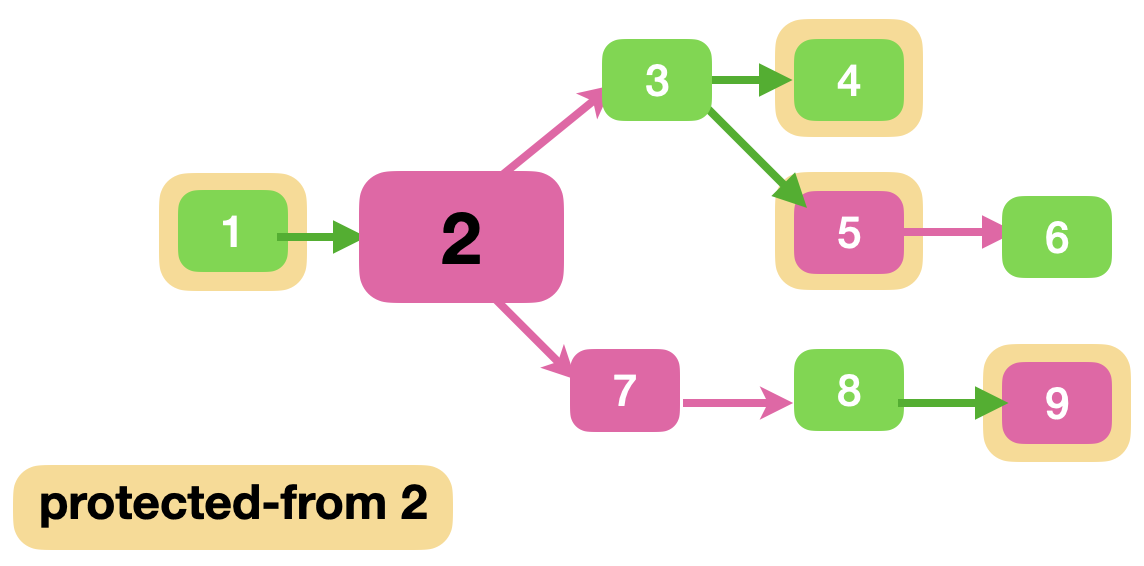
\includegraphics[width=\linewidth]{diagrams/prfC.png}
} 
&
\resizebox{4.5cm}{!}{
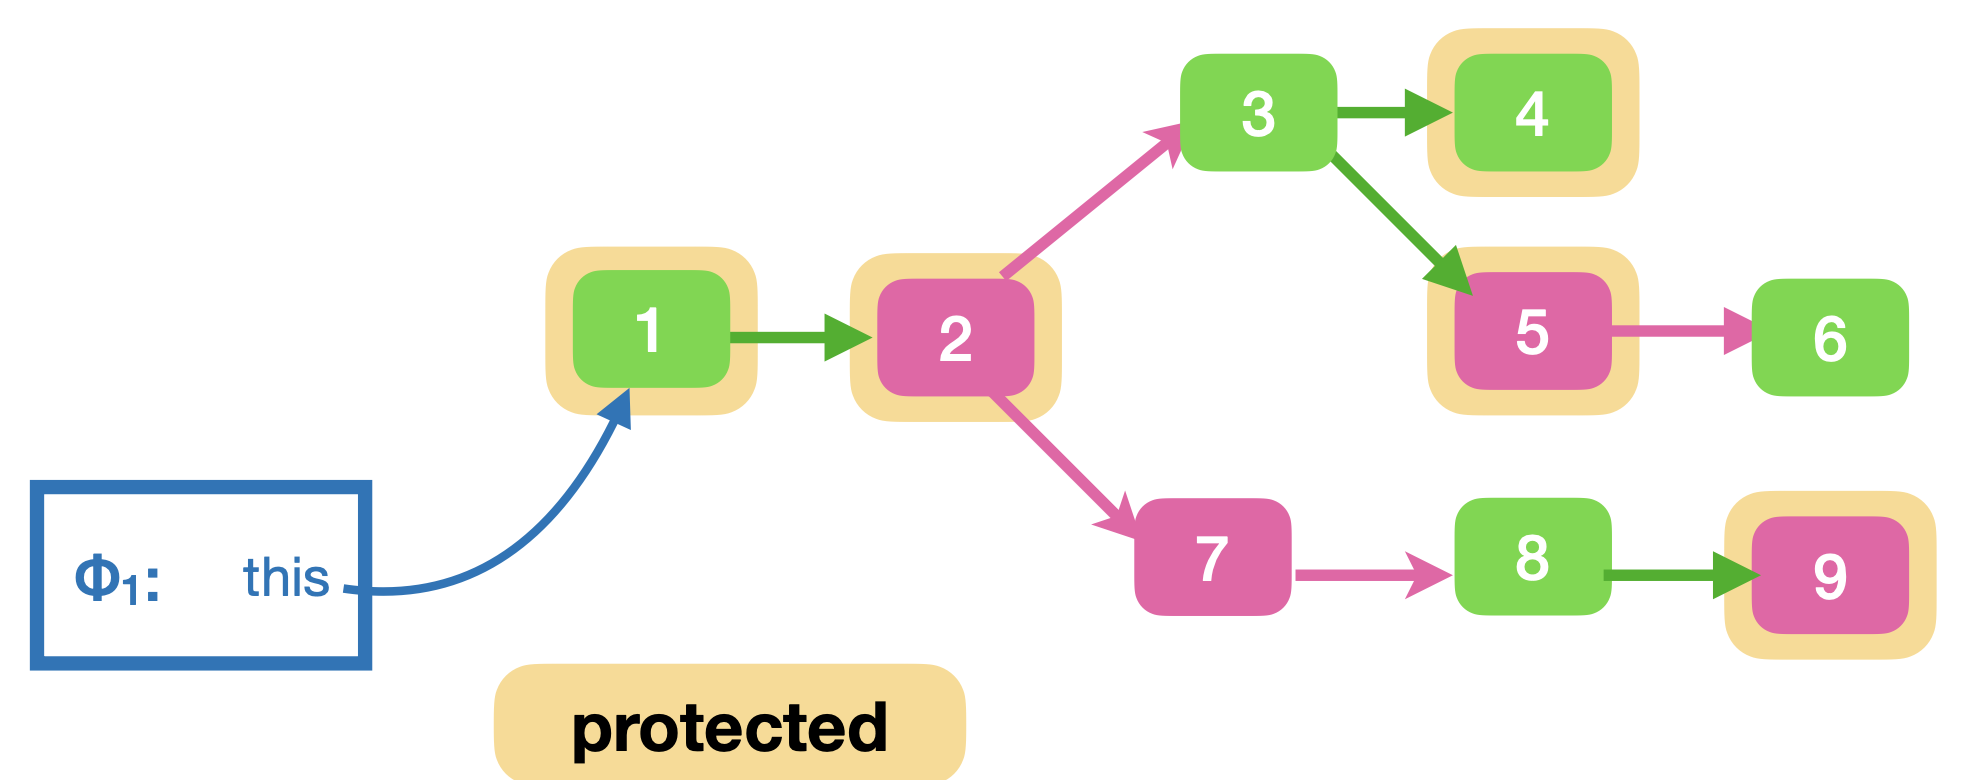
\includegraphics[width=\linewidth]{diagrams/prtFirst.png}
}
&
\resizebox{4.5cm}{!}{
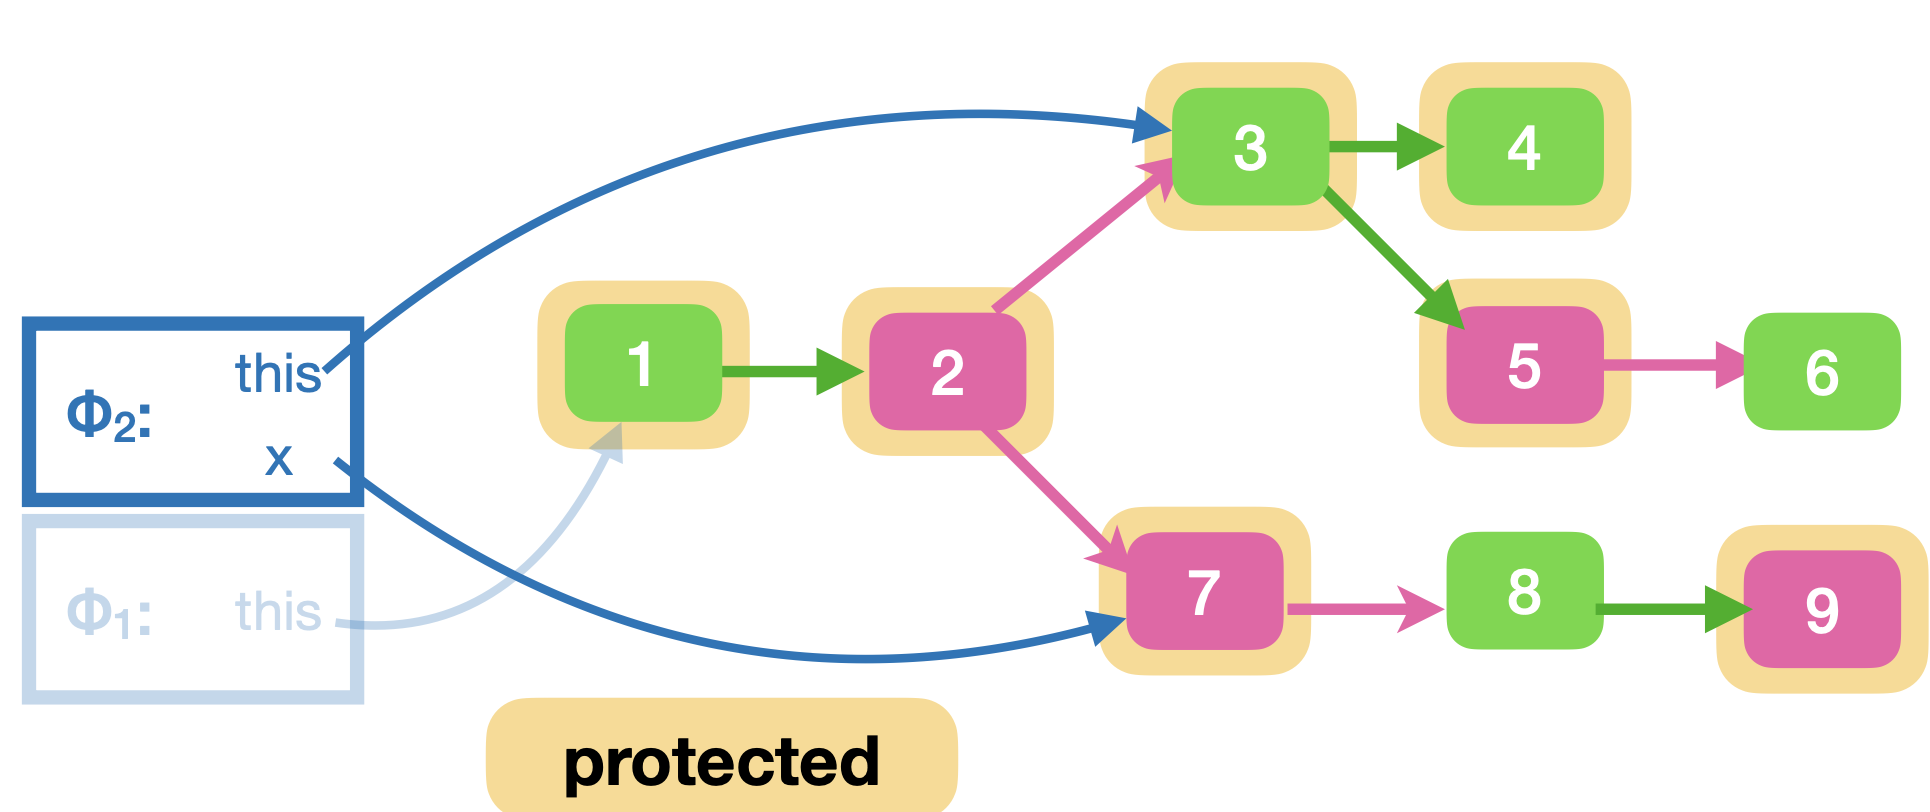
\includegraphics[width=\linewidth]{diagrams/prtSecond.png}
}
\\
\hline
protected from object $o_2$
&
protected  with top frame $\phi_1$
&
protected  with top frame $\phi_2$
\\
\hline \hline
\end{tabular}
\caption{Protected from and Protected. Pink and green squares are external and internal objects, respectively. Connecting straight arrows  indicate fields. Blue boxes are frames on the stack. Protected objects are  highlighted in yellow. 
 The left pane shows a heap with objects $o_1$-$o_9$.
 Here  $o_1$, $o_4$, $o_5$ and $o_9$ 
are protected from $o_2$. 
 The middle pane {shows the same heap and a stack with frame  $\phi_1$} whose receiver,   \prg{this},  points to $o_1$. Here 
 $o_1$, $o_2$, $o_4$, $o_5$ and $o_9$  are protected. 
 The right pane {shows the same configuration, but after pushing frame  $\phi_2$}, whose receiver,  \prg{this},  and local variable, \prg{x}, point to $o_3$ and  $o_7$, respectively.
 Here $o_3$ and $o_7$ are protected, in addition  to  the objects protected in the previous pane.
}
   \label{fig:ProtectedBoth}
 \end{figure}
 

\subsection{2$^{nd}$ Challenge: Specification of tamed effects}
\label{sect:approach:scoped}
How can we express the guarantee that effects are \tamed?  
 In particular, when such effects can be the outcome of the execution of more than one method? 
 Traditional,  {per-method} PRE/POST conditions {cannot guarantee} %specifications cannot express guarantees
  that two or more of our methods won't interact to produce an untamed effect. 
We build on the concept of history invariants \cite{liskov94behavioral,usinghistory,Cohen10} and define

\begin{description}
\item[{Scoped invariants}]  
{$\TwoStatesN  {\overline{x:C}}  {A}$} expresses that if a {state} $\sigma$ 
 has objects $\overline x$ of class $\overline C$, and satisfies $A$, then all $\sigma$'s \emph{scoped  future  states} will  {also} satisfy  {$A$}. 
The scoped future contains all % \sdN{future} 
 states which can be reached through any steps, including further method calls and returns, but stopping before returning  from the call active in $\sigma$ \footnote{{Here lies the difference to history invariants, which consider \emph{all} future states, including returning from the call active in $\sigma$.}}  --  \cf Def  \ref{def:shallow:term}.
{For} $\sigma$ and its scoped future   we only consider external states -- \cf Def \ref{def:necessity-semantics}.
\end{description}

    
\label{s:bank}



\begin{example}
\label{s:bankSpecEx}
The following scoped invariants\\
$\strut \SPSP\ \ \   S_1\ \  \triangleq \ \ \TwoStatesN {\prg{a}:\prg{Account}}  {\inside{\prg{a}}} $ 
\hspace{1.1cm}
$\strut  \SPSP\ \ \   S_2\ \  \triangleq \ \ \TwoStatesN  {\prg{a}:\prg{Account}}  {\inside{\prg{a.key}}} $ 
% \\
%$\strut  \SPSP   S_3\ \  \triangleq \ \ \TwoStatesN {\prg{a}:\prg{Account},\prg{b}:\prg{int}}  {\inside{\prg{a}} \wedge \prg{a.\balance}=\prg{b}}  $
\\
$\strut  \SPSP\ \ \   S_3\ \  \triangleq \ \ \TwoStatesN{ \prg{a}:\prg{Account},\prg{b}:\prg{int} } {\inside{\prg{a.key}} \wedge \prg{a.\balance} \geq \prg{b} } $ 
% \end{tabular}
%}

\noindent
%specifications
 guarantee that   accounts are not leaked  ($S_1$), \ \ keys are not leaked  ($S_2$), \ \ the balance does not decrease unless there is unprotected access to the key  ($S_3$).
 % $\strut  \SPSP  S_1$:\   accounts are not leaked,  \hspace{1.1cm}
%$\strut   \SPSP S_2$:\    keys are not leaked,\\
%%$\strut \SPSP  S_3$:\  the balance is not modified unless there is unprotected access to the account,  \\%while 
%$\strut \SPSP  S_3$:\   the balance does not decrease unless there is unprotected access to the key.  
%
\end{example} 


 
 \vspace{.05cm}

 
\noindent
{\textbf{\sdN{Scoped invariants are} \emph{conditional}}:}  They ensure that assertions are \emph{preserved}, but unlike object invariants, they do not guarantee that they always hold.
\ \Eg   \prg{buy} cannot assume $\inside{a.\prg{key}}$ holds on entry, but   guarantees that if it holds on entry, then  it will still hold on exit.

 
 \begin{example}
 We   use the features from the previous section to specify methods. 

{\sprepost
		{\strut \ \ \ \ S_4} 
		{   \protectedFrom{\prg{this}.\prg{\myAccount}.\prg{key}} {\prg{buyer}} \wedge \prg{this}.\prg{\myAccount}.\prg{\balance}=b
		 }
		{\prg{public Shop}} {\prg{buy}} {\prg{buyer}:\prg{external}, \prg{anItem}:\prg{Item} }
		{ 
		  %\protectedFrom{\prg{this}.\prg{\myAccount}.\prg{key}} {\prg{buyer}} \wedge 
		  \prg{this}.\prg{\myAccount}.\prg{\balance}\geq b
		 }
}

\noindent
$S_4$  guarantees that if the % account's 
key was protected from \prg{buyer} before the call, then the balance will not decrease. %SD is shorter, but I hope ckear eniugh  \prg{buy} will not decrease the %shop's account  balance. 
 It does \emph{not} guarantee \prg{buy} will only be called when $\protectedFrom{\prg{this}.\prg{\myAccount}.\prg{key}} {\prg{buyer}}$ holds. 
As a  public method,  \prg{buy}  can be invoked by external code that ignores all specifications.
\end{example}

% \vspace{.05cm}

\begin{example}
We illustrate the meaning of our specifications  using three  versions of a class \prg{Account}  from  \cite{OOPSLA22} 
as part of our internal module \Mshop. 
To differentiate, we rename \Mshop  as $\ModA$,  $\ModB$, or $\ModC$. 
All use the same \prg{transfer} method for withdrawing money.
%All use the same method \prg{transfer} to  withdraw money, only when supplied with the key.
%\forget{All versions {use the same method \prg{transfer} to} allow  withdrawal of money, only when supplied with the key to the account.
%All use the same method \prg{transfer} to  withdraw money, only when supplied with the key.}
% removed class Key -- it does not need to be internal 
\begin{lstlisting}[mathescape=true, language=Chainmail, frame=lines]
module $\ModA$      
  class Shop   ... as earlier ...
  class Account
    field blnce:int 
    field key:Key
    public method transfer(dest:Account, key':Key, amt:int)
       if (this.key==key')   this.blnce-=amt; dest.blnce+=amt
     public method set(key':Key)
       if (this.key==null)  this.key=key'
\end{lstlisting}

Now consider  modules \ModB and \ModC which differ from \ModA only in their \prg{set} methods. Whereas \ModA 's key is immutable, \ModB allows any client to reset an account's key at any time, and \ModC requires the existing key in order to change it.
  

\begin{tabular}{lll}
\begin{minipage}[b]{0.40\textwidth}

\begin{lstlisting}[mathescape=true, language=Chainmail, frame=lines]
$\ModB$
public method set(key':Key)
  this.key=key'
\end{lstlisting}
\end{minipage}
&\ \ \  \ \   &%
\begin{minipage}[b]{0.48\textwidth}
\begin{lstlisting}[mathescape=true, language=chainmail, frame=lines]
$\ModC$
public method set(key',key'':Key)
  if (this.key==key')  this.key=key''
\end{lstlisting}
\end{minipage} 
\end{tabular}

{Thus, in all three modules, the key is an object capability which \emph{enables} the withdrawal of the money. 
Moreover, in $\ModA$ and $\ModC$, the key
{is a capability} used to  \emph{tame} withdrawal of money, preventing those without it from getting the money from the account.}
Crucially,  in $\ModB$ the key \emph{does not tame} withdrawal of money.
Using $\ModB$, it is possible to start in a state where the account's key is unknown, modify the key, and then withdraw the money. 
Code  {such as}
\\ 
$\ \strut \hspace{.2in} $ \prg{k=new Key;  acc.set(k); acc.transfer(rogue\_accnt,k,1000)} 
\\ 
is enough to drain  \prg{acc} in \ModB without knowing the \password.\footnoteSD{CAREFUL: we had 
$\ \strut \hspace{.01in} $ \prg{an\_account.set(42); an\_account.transfer(rogue\_accnt,42)} but this was type incorrect!}
 %
% \emph{Emergent behaviour} is key here: 
Even though % the method 
\prg{transfer} in  \ModB is ``safe'' when considered in isolation, it is not safe when considered in conjunction with other methods from the same module. 

Our  specifications  rule  out \ModB while permitting \ModA and
\ModC:
No module  satisfies $S_1$. Modules $\ModA$ and $\ModC$ satisfy $S_2$ and $S_3$, while $\ModB$ satisfies neither $S_2$ nor $S_3$.
\end{example}
 
\forget{% for the time being at least
{ \noindent
 Our specifications are  in terms of the complete module, rather than per-method.
 They talk about externally observable effects (\eg the key stays protected), 
 % the account's balance may increase), 
 rather than about  individual methods (\eg\, \prg{set}). %  or \prg{transfer}).
{Thus,   they can characterize  any 
module with  accounts which have a % {\textit{implementation}} of a bank account with a 
 \balance~and a \password -- even as ghost fields --}  irrespective of the API offered.
} }% , services  exported, or  dependencies on other parts of the system.\footnoteSD{does this come from OOPSLA? if so we need to rephrase}
%\notesep
%Adherence to   specifications is not monotonic:
%{Eg, while  \ModA satisfies $S_3$, the addition of \prg{set} lead to \ModB, which does not.}
%% Adding a method to a module does not necessarily preserve such adherence,
%% \eg adding method \prg{set} in module \ModB breaks 
%%SD removed the below. When we changed the invaraints to have the same assertion re and post it no longer hel
%\forget{, and while separate methods may adhere to a  specification, their combination does
%not necessarily do so. 
%{For example, \ModB's  \prg{tansfer} and \prg{set} satisfy $S_3$, but their interplay does not.}
%%In this sense, and, similar to OOPSLA'22, our  specifications capture a module's \emph{emergent behaviour}. 


  
  \subsection{3$^{rd}$ Challenge:  A Hoare logic} %  for external calls} %  (using scoped invariants)}
 \label{sec:howThird}


 
 \vspace{.1cm}
 
We now move to the  verification of $S_4$. 
The challenge is how to reason  about the external call on line 8. %, even though we do not have a specification for \prg{pay}
% the  {called method}, we know that the effects of the call are tamed according to the module's scoped invariants. 
% SD BELOW is wrong. left just in case we want to adapt ir.
% That is expressed in the  simplified Hoare rule below -- \cf. Fig.\ref{f:external:calls}. 
% 
%  $\inferruleNoName  
% 	{ 
%   	   {\TwoStatesN {\overline {x:D}} {A}}\ \   \mbox{is part of $M$'s specification}
%        }
%	{   \triple { \    { \external{y_0}} \,     \wedge \,  \overline{x:D}\  \wedge\  A\ }  
%						{ \ u:=y_0.m(y_1,.. y_n)\    }
%						{ \    A  \ }
%						\  \  ...
%         }
%$
%
%\vspace{.05cm}
% 
% Now  revisit the external call from line 9 in Section \ref{sec:shop}. Our argument is that 
We aim to establish a Hoare triple of the form:
 \\
$\strut \ \ \ \ \ \ \ \ \ \ \  \{\  \ { \external{\prg{buyer}}} \ \wedge\ {\protectedFrom {\prg{this.\myAccount.key}} {\prg{buyer}}\ \wedge\ {\prg{this.\myAccount.\balance}}= b    }\ \  \}$\\
$\strut \ \ \ \ \ \ \ \ \ \ \   \ \ \ \ \ \ \ \ \ \ \ \ {\ \prg{buyer.pay(this.accnt,price)}   \ } $\\
$\strut \ \ \ \ \ \ \ \ \ \ \  \{\  \ \  {\prg{this.\myAccount.\balance}} \geq  b \  \  \}$ 
\\
The intuitive reasoning is as follows: if the shop's account's key is protected from \prg{buyer} (A from earlier), and the module satisfies $S_3$ (B), then after the call, the account's balance will not decrease (C).
%
However, application of $S_3$ is not straightforward. 
%While $S_3$ preserves ${\inside{\prg{a.key}}} \wedge ...$,
%Application of $S_3$ 
It requires ${\inside{\prg{a.key}}} \wedge ...$,  but  the call's precondition only guarantees $\protectedFrom{\prg{this.\myAccount.key}}{\prg{buyer}}$. 
%To apply $S_3$, we would need to know ${\inside{\prg{this.\myAccount.key}}}$, but we only know $\protectedFrom{\prg{this.\myAccount.key}}{\prg{buyer}}$.


%, while we  need the stronger property  ${\inside {\prg{this.\myAccount.key}}}$. 

While we do \susan{not} know whether \prg{a.key} is protected during  execution of \prg{buy}\footnote{For instance, one of the clients may have access to it.}, we can be certain it is protected during execution of \prg{pay}.  This is so, because the objects accessible during \prg{pay} are those visible from its arguments (\ie \prg{buyer} and \prg{price}).
% \footnote{Generally, more objects are protected from the viewpoint of the called function than from that of the caller -- \cf  Fig. \ref{fig},}

%To express this difference, 
We define the adaptation operator $\FIXSymbolA$, which translates an assertion from the viewpoint of the called function to that of the caller. 
Specifically, $\PushAS y A$ ensures that $A$ holds when the variables $\overline{y}$ (where $\overline{y}$ stands for $y_1, ..., y_n$) have been pushed onto a new frame. 
For example, $\PushAS y {(\inside \re)} = \protectedFrom \re {\overline{y}}$ for any term $\re$ (see  \susan{Def. \ref{def:chainmail-protection-from}})
 and Lemma \ref{lemma:push:ass
}).
%
In this case, we have:\\  {\small{$\strut \ \ \ \PushASLong {\{\prg{buyer},\prg{price}\}}  {(\inside {\prg{this.\myAccount.key}})}$
 \ = \  $\protectedFrom {\prg{this.\myAccount.key}} {(\prg{buyer},\prg{price})}$.}}
 \\
 and with this, we \emph{can} apply $S_3$.
 %
 {Below  a  Hoare logic rule  dealing with external calls - \cf. Fig.\ref{f:external:calls}.} % where $\overline y$ stands for $y_1$,,, $y_n$ -
 
 $\inferruleNoName  
 	{ 
   	   {\TwoStatesN {\overline {x:D}} {A}}\ \   \mbox{is part of $M$'s specification}
        }
	{   \triple { \    { \external{y_0}} \,     \wedge \,  \overline{x:D}\  \wedge\  {\PushASLong {(y_0,\overline y)}{A}} \ }  
						{ \ u:=y_0.m(\overline y)\    }
						{ \    {\PushASLong {(y_0,\overline y)}{A}}  \ }
						\  \  ...
         }
$

 
 
 
%   \subsection{4$^{th}$ Challenge: A Hoare Logic for Proving that modules adhere to specifications} %  (using scoped invariants)}
%
% We now revisit the meaning of scoped invariants: 
%  {$\TwoStatesN  {\overline{x:C}}  {A}$} expresses that if an external {state} $\sigma$ 
%% with objects $\overline x$ of class $\overline C$ 
% satisfies $\overline {x:A} \wedge A$, then all its \emph{scoped} external future  states will  {also} satisfy  {$A$}. 
%\Eg if $\sigma$ was an external state executing a call to \prg{Shop::buy}, then a \emph{scoped} external future  state
% could be an external state reachable 
%after the return from \prg{Shop::buy}, but could also be reachable
%during execution of the external call \prg{pay}.
%This means that we are  interested in the states before %and after a method (or statements)
%statements, \emph{but  also}  in the external states reachable \emph{during} execution of these statements. 
%%of that method (or statements).
%To accommodate this, we extend   traditional Hoare triples to quadruples of  form\\
% $\strut \ \hspace{4cm} \quadruple {A} {\, stmt\, }{A'} {A''}$\\  
% promising that if a state satisfies $A$ and executes $stmt$, any terminating state will satisfy $A'$, and 
% and  any intermediate external states reachable during execution of $stmt$ satisfy    $A''$ -- \cf Def. \ref{def:hoare:sem}.
%% same as above, but ugly line break:
%% terminating execution of $stmt$ in  states satisfying $A$  reaches    final states satisfying $A'$, and any intermediate external states reachable during execution of $stmt$ satisfy    $A''$ -- \cf Def. \ref{def:hoare:sem}.
%
%\vspace{.05cm}
%
%The Hoare logic rule from earlier dealing with external calls is:
% 
% $\inferruleNoName  
% 	{ 
%   	   {\TwoStatesN {\overline {x:D}} {A}}\ \   \mbox{is part of $M$'s specification}
%        }
%	{   \quadruple { \    { \external{y_0}} \,     \wedge \,  \overline{x:D}\  \wedge\  {\PushASLong {(y_0,\overline y)}{A}} \ }  
%						{ \ u:=y_0.m(\overline y)\    }
%						{ \   {\PushASLong {(y_0,\overline y)}{A}}  \ }
%						{\  A  \ }
%         }
%$

\vspace{.4cm}

To develop our logic, we   take  a  Hoare logic %of  triples, 
which does not {have} the concept of protection.
%We then extend this logic as follows: We define an embedding into our quadruples. 
%and allow method specifications which also talk about intermediate external states.
We  extend it through % substructural rules, and 
rules talking about protection, and internal and external calls 
-- \cf Figs. \ref{f:underly} -  \ref{f:calls}. % \ref{f:wf}.
A module is well-formed, if  its invariants are well-formed,    its public methods preserve   its invariants, and  all  methods satisfy their specifications - \cf  Fig.  \ref{f:wf}.
An invariant is well-formed if   it is \emph{encapsulated}, \ie can only be invalidated by internal code
-- \cf Def. \ref{d:encaps}. 
A method preserves an assertion   if it preserves it   from pre- to  post-states and also to any intermediate external state.
 Our extension preserves soundness of the  Hoare logic --  \cf   
 Thms.  \ref{l:triples:sound},  \ref{thm:soundness}.




% \vspace{.05cm}
%A module is well-formed, if  its invariants are well-formed,    its public methods preserve   its invariants, and  all  methods satisfy their specifications - \cf  Fig.  \ref{f:wf}.
%% 
%An invariant is well-formed if   it is \emph{encapsulated}, \ie can only be invalidated by internal code
%-- \cf Def. \ref{d:encaps}. 
%A method preserves an assertion   if it preserves it   from pre- to  post-states and also to any intermediate external state.

%\vspace{.05cm}
%%  \se{!!!WE HAVE REMOVED S\_3!!! I CAN REMOVE THE MENTION HERE}
%%\sd{Good catch! Replace with $S_2$ Note that I removed the next paragraph, though.}
%
%\Eg to prove  that method \prg{Shop::buy} satisfies  {$S_2$}  we  need to prove:
%\\
% {\footnotesize{
%%$\strut \ \ \ \ \ \ \ \ \ \ \ \quadruple {A_1  \wedge \inside{\prg{a}} } {\ stmt\_b  \ } {\inside{\prg{a}}} { \inside{\prg{a}}} $
%%\\
%%$\strut \ \ \ \ \ \   \ \  \quadruple {A_1  \wedge  \inside{\prg{a.\password}} } {\  stmt\_buy  \  } {\inside{\prg{a.\password}}}  {\inside{\prg{a.\password}}}$
%%\\
%$\strut \ \ \ \ \ \  \ \  \ \ \   \quadruple {A_1  \wedge  \inside{\prg{a.key}} \wedge  \prg{a.\balance}\!=\!{\prg{b}} } {\   stmt\_b  \  } {\inside{\prg{a.key}} \wedge  \prg{a.\balance}\!=\!\prg{b}}   
%                         {  \inside{\prg{a,key}} \wedge  \prg{a.\balance}\!=\!\prg{b} }$
%%\\
%%$\strut \ \ \ \ \ \   \ \   \quadruple {A_2  \wedge  \inside{\prg{a.\password}} \wedge  \prg{a.\balance}\!\geq\!{\prg{b}} } {\  stmt\_buy  \  } {\inside{\prg{a.\password}} \wedge  \prg{a.\balance}\!\geq\!{\prg{b}}}  
%%   { \inside{\prg{a.\password}}\wedge  \prg{a.\balance}\!\geq\!{\prg{b} }}$
%  }}
%\\
%%and similar for {$S_3$}. Here we used   
%with  $A_1 \triangleq $ % {\footnotesize{
%{{\prg{this}:\prg{Shop}, \prg{buyer}:\prg{external}, \prg{anItem}:\prg{Item}, \prg{a}:\prg{Account}$
%$, \prg{b}:\prg{int}}} and $stmt\_b$   short for  the body of \prg{buy}.
% 
%% \vspace{.2cm}
%%Quadruples are also used in method specifications, \eg we specify \prg{transfer} through
%%\\
%%$\strut \ \ \ \ \ \  \ \  \ \ \  { \mprepostLongN {A_3}{\prg{public}\ \prg{Account}}{\prg{transfer}}{params}{A_4} {true} }$
%%\\
%%with shorthands  $params \triangleq$ \prg{dest:Account}, \prg{key':Key}, \prg{amt:int}, and 
%%$A_3  \triangleq$  $\prg{key'}=\prg{this.\password} \wedge \prg{dest}\neq \prg{this}$
%%$\wedge\, b, b':\prg{int}$
%%$\, \wedge\, \prg{this.\balance}=b$ 
%%$\, \wedge\,  \prg{dest.\balance}=b'$, 
%% and $A_4 \triangleq$  
%% $\prg{this.\balance}=b-\prg{amt} \wedge \prg{dest.\balance}=b'+\prg{amt}$.
%%%For this specification, we need to prove\\
%%%$\strut \ \ \ \ \ \ \ \ \ \ \ \quadruple {\ \prg{this}:\prg{Account}\, \wedge\, params\, \wedge\, A_3  \  } {\ stmt\_{tr}  \ } {A_4} { true} $
%%%\\
%%%where $stmt\_{tr}$ is short for the body of  \prg{transfer}.

\subsection*{Summary}

In our threat model, external objects can execute arbitrary code, invoke any public internal methods, have potentially access to any other external object, and may collude with one another  in any conceivable way.
Our specifications are conditional: they do not guarantee that certain effects will never occur, but they ensure that specific effects will only happen if certain conditions were met prior to the execution of the internal code.
 
The key ingredients of our work are: a) the concept of protection ($\protectedFrom {x} {y}$ and $\inside {x}$), b) the \scoped invariants (${\TwoStatesN {\overline {x:D}} {A}}$), and c) the adaptation operator ($\FIXSymbolA$).
In the remaining sections, we discuss all this in more detail.

% \vspace{0.1cm}
% \noindent
 

 
\footnoteSD{Do we want to talk about the challenges in the proof, and the fact that we reason using sufficient but have necessary in mind.}
\forget{The proof that the extended Hoare logic is sound is interesting, because we are arguing about the soundness of two interrelated systems: 
 the per-statement  Hoare logic, as well as the {entire} module's logic.
Moreover, we need to cater for the possibility that external calls eventually call public methods of the module, which in their turn make external calls etc.
For this we define a new measure of execution ...}

 
 


\section{The Meaning of Necessity}
\label{s:semantics}

 
In this section we define {the}  \Nec specification language.  
We first define an underlying programming language, \Loo (\S \ref{sub:Loo}).
We then define an assertion language, \SpecO, which can talk about the
contents of the state, as well as about provenance, permission and
control (\S \ref{sub:SpecO}).  Finally, we define the syntax and
semantics of our full language for writing \Nec
specifications (\S \ref{s:holistic-guarantees}).


\subsection{\Loo}
\label{sub:Loo} 
%\jm[TODO: mention the type system and the restriction on external method calls]{}
%% We introduce a simple object-oriented language, \Loo, upon 
%% which our specification language sits.
 \Loo is a \jm[removed: formal model of a]{} {small}, imperative, sequential, 
class based, typed, object-oriented language, whose
\sdS{fields are private to the class where they are defined.}
\Loo is straightforward
%Given its simplicity, %  the simplicity of \Loo, we do notdefine it here, instead, 
% we direct the reader to
\jm[]{and the full definition can be found in the appendices of the full paper \cite{necessityFull}.}
%Appendix \ref{app:loo} contains 
%the full definitions.
%%and introduce here only % syntax and operational semantics.
%% the concepts relevant to the
%%treatment of the open world guarantees.
%\jm[]{\Loo fields are private in the way fields in Java are private,
%the privacy is class-wide, i.e. they may only be read or written to by 
%objects of the same class.}
\Loo is based on \LangOO 
\cite{FASE}, with some small variations, as well as 
the addition of  % while \LangOO is untyped, \Loo 
 a simple type system -- more in \ref{types}.
%has type based restrictions on external access to private data.}
%\sophiaPonder[added]{Note that the operational semantics only allows filed
%update if the receiver and the object being updated belong to the same class,
%and only allows method calls }
%
%
A \Loo state $\sigma$ consists of a 
heap $\chi$, and a  {stack $\psi$ which is a sequence of frames}.
A frame $\phi$ consists of
local variable map, and a continuation, \ie a sequence of statements to be executed.
 A statement may assign to variables, create new objects and push them to the heap, 
perform field reads and writes on objects,  or
 call methods on those objects. 

%Program 
 Modules are mappings
from class names to class definitions. 
Execution 
%takes place
is in the context of  a module $M$ and   a state $\sigma$,
%It is % Execution
 defined via unsurprising small-step semantics of the form \ \ 
   $M, \sigma \leadsto \sigma'$.
The   top frame's continuation contains the statement to be % currently being 
executed next.
 % chopped, as generic 
 % There are several properties  of \Loo that are important to the central topic of this paper. 
 
As discussed in \S \ref{s:approach}, %we are interested in 
{open world specifications need to be able to provide}
guarantees which hold
during execution of an internal, 
known, trusted module $M$ when linked together with any
unknown, untrusted, module $M'$. These guarantees need only hold 
when the external module is executing; we are not concerned if they are
temporarily broken by the internal module. Therefore, we are only interested in states where the
executing object (\prg{this}) is an external object. 
To express our focus on external states, we define the  \emph{external states semantics}, of the form 
$\reduction{M'}{M}{\sigma}{\sigma'}$, where $M'$ is the external
module, and $M$ is the internal module, and where we
collapse all internal steps into one single step.

 

\begin{definition}[External States Semantics]
\label{def:pair-reduce}
For  
% If we say "internal module", it is sounds as something makes the module be internal
  modules $M$,  $M'$, and % program
   states $\sigma$, $\sigma'$, 
we say that $\ \ \ \ \ \ \ \ \reduction{M'}{M}{\sigma}{\sigma'}\ \ \ \ \ \ \ \ $ if and only if there exist 
$n\in\mathbb{N}$, and states $\sigma_0$,...$\sigma_n$, such that
\begin{itemize}
\item
$\sigma$=$\sigma_1$, and  $\sigma'$=$\sigma_n$,
\item
$M' \circ M, \sigma_i \leadsto \sigma_{i+1}$  \ \ \ for all $i\in [0..n)$,
\item
$\class{\sigma}{\scd{\prg{this}}}, \class{\sigma'}{\scd{\prg{this}}}\in M'$,
\item
$\class{\sigma_i}{\scd{\prg{this}}} \in M$\ \ \ for all $i\in (1..n)$.
\end{itemize} 
\end{definition}
The function $\class{\sigma}{\_}$ is overloaded:
  applied to a variable, 
$\class{\sigma}{x}$  looks up the variable $x$ in the top frame of $\sigma$, and returns the 
class of the corresponding object in the  heap of $\sigma$;
%while  
applied to an address, $\class{\sigma}{\alpha}$  returns
the class of   the object referred by address $\alpha$ in the heap of $\sigma$.
 The module linking operator $\circ$, applied to two modules, $M'\circ M$, 
 combines the two modules into one module in the obvious way, provided their
domains are disjoint.
Full details in \jm[]{can be found in the appendices of the full paper \cite{necessityFull}.} %Appendix \ref{app:loo}.
\begin{figure}[htb]
\begin{tikzpicture}[->,>=stealth',shorten >=1pt,auto,node distance=9mm,
                    thick,
                    external node/.style={circle,draw,minimum size=7mm,font=\sffamily\Large\bfseries, color=blue, fill = blue, text = black, fill opacity = 0.5},
                    internal node/.style={circle,draw,minimum size=7mm,font=\sffamily\Large\bfseries, color=orange, fill = orange, text = black, fill opacity = 0.5}]
    
	\node[external node] (a) {1};
	\node[internal node] (b) [right = of a] {2};
	\node[external node] (c) [right = of b] {3};
	\node[external node] (d) [right = of c] {4};
	\node[internal node] (e) [right = of d] {5};
	\node[internal node] (f) [right = of e] {6};
	\node[external node] (g) [right = of f] {7};
	\node[internal node] (h) [right = of g] {8};
	\node[external node] (i) [right = of h] {9}; 

	\path[every node/.style={font=\sffamily\small}]
		(a) edge[bend left] node [above] {} (b)
		(b) edge[bend left] node [above] {} (c)
		(c) edge[bend left] node [above] {} (d)
		(d) edge[bend left] node [above] {} (e)
		(e) edge[bend left] node [above] {} (f)
		(f) edge[bend left] node [above] {} (g)
		(g) edge[bend left] node [above] {} (h)
		(h) edge[bend left] node [above] {} (i);
\end{tikzpicture}
\begin{tikzpicture}[->,>=stealth',shorten >=1pt,auto,node distance=9mm,
                    thick,
                    external node/.style={circle,draw,minimum size=7mm,font=\sffamily\Large\bfseries, color=blue, fill = blue, text = black, fill opacity = 0.5},
                    internal node/.style={circle,draw,minimum size=7mm,font=\sffamily\Large\bfseries, color=orange, fill = orange, text = black, fill opacity = 0.2, draw opacity = 0.5}]
    
	\node[external node] (a) {1};
	\node[internal node] (b) [right = of a] {2};
	\node[external node] (c) [right = of b] {3};
	\node[external node] (d) [right = of c] {4};
	\node[internal node] (e) [right = of d] {5};
	\node[internal node] (f) [right = of e] {6};
	\node[external node] (g) [right = of f] {7};
	\node[internal node] (h) [right = of g] {8};
	\node[external node] (i) [right = of h] {9}; 

	\path[every node/.style={font=\sffamily\small}]
		(a) edge[bend left=46] node [above] {} (c)
		(c) edge[bend left=46] node [above] {} (d)
		(d) edge[bend left=46] node [above] {} (g)
		(g) edge[bend left=46] node [above] {} (i);
\end{tikzpicture}
   \caption{External States Semantics
     (Def. \ref{def:pair-reduce}),  %
     % 
     (A) $\exec{{\color{hotpink}M'} \circ {\color{lightseagreen}M}}{\sigma_1}{\ldots}\leadsto \sigma_9$ \ \ \ and \ \ \ 
     (B) $\reduction{{\color{hotpink}M'}}{{\color{lightseagreen}M}}{\sigma_2}{\ldots}\leadsto \sigma_9$, \ \ \ 
     \\
     where $\class{{\color{lightseagreen}\sigma_1}}{\scd{\prg{this}}}$,$\class{{\color{lightseagreen}\sigma_3}}{\scd{\prg{this}}}$,$\class{{\color{lightseagreen}\sigma_4}}{\scd{\prg{this}}}$,$\class{{\color{lightseagreen}\sigma_7}}{\scd{\prg{this}}}$,$\class{{\color{lightseagreen}\sigma_8}}{\scd{\prg{this}}}\in {\color{lightseagreen}M}$,\\
     and where $\class{{\color{hotpink}\sigma_2}}{\scd{\prg{this}}},\class{{\color{hotpink}\sigma_5}}{\scd{\prg{this}}} 
     \class{{\color{hotpink}\sigma_6}}{\scd{\prg{this}}},\class{{\color{hotpink}\sigma_9}}{\scd{\prg{this}}}\in {\color{hotpink}M'}$.
    %  (c) $\reduction{{\color{orange}M'}}{{\color{blue}M}}{\sigma_1}{\ldots}\leadsto \sigma_8$
    }
   \label{fig:VisibleStates}
 \end{figure}
 
Fig. \ref{fig:VisibleStates} inspired by \citeasnoun{FASE} provides a simple graphical description of 
our external states semantics: (A) is the ``normal'' execution after 
linking two modules into one: \ $M' \circ M, ... \leadsto ...$ whereas (B) is the
 external states execution when $M'$ is external,\   $\reduction{M'}{M}{...}{...}$.
Note that whether a module is external or internal depends on %our
perspective -- nothing in a module itself renders it internal or external. For example, in
 $\reduction{M_1}{M_2}{...}{...}$ the external module is $M_1$,
  while in  $\reduction{M_2}{M_1}{...}{...}$  the external module is $M_2$.

We  use the notation\ \  $\reductions{M'}{M}{\sigma}{\sigma'}$ \ 
to denote zero or more  steps starting at state $\sigma$ and ending at state $\sigma'$, in the context of internal module 
$M$ and external module $M'$.
 %Not only are we unconcerned 
%with internal states,  we are also unconcerned with  states which cannot ever arise from execution.
We are \jm[]{not} concerned with internal states or states that can never arise.
{A state $\sigma$ is \emph{arising},}  written $\arising{M'}{M}{\sigma}$, {if it  may arise by external states} execution
starting at some initial configuration:



\begin{definition}[Arising  States]
\label{def:arising}
For   modules $M$ and  $M'$, a % program
 state $\sigma$ is 
called an \emph{arising} state, formally \ \ \ $\arising{M'}{M}{\sigma}$,\ \ \ 
if and only if there exists some $\sigma_0$ such that $\initial{\sigma_0}$ and
$\reductions{M'}{M}{\sigma_0}{\sigma}$.
\end{definition}

An \emph{Initial} state's heap
contains a single object of class \prg{Object}, and
its  stack   consists of a single frame, whose local variable map is a
mapping from \prg{this} to the single object, and whose continuation is  any statement.
(See Definition %s \ref{def:initial} and 
\ref{def:arising} and the appendices of the full paper \cite{necessityFull}).


\paragraph{Applicability} 
{While our work is based on 
  a simple, imperative, typed, object oriented}
language with unforgeable addresses and private fields, we believe
 that % our approach
 it is applicable to several programming paradigms, and 
 that   unforgeability and privacy
 can be replaced 
 by lower level mechanisms such as capability machines \cite{vanproving,davis2019cheriabi}.

\subsection{\SpecO}
\label{sub:SpecO}

\SpecO is \jm[removed: a subset of the \emph{Chainmail} assertions language, \ie]{}
a basic assertion language extended with
object-capability assertions. 


\subsubsection{Syntax of \SpecO}
The syntax of \SpecO   is given in
Definition \ref{f:chainmail-syntax}.
An assertion may be an expression,   a query of the defining class of
  an object, the usual connectives and quantifiers, along 
with three non-standard assertion forms:
(1) \emph{Permission} and (2) \emph{Provenance}, inspired by the capabilities literature, and
(3) \emph{Control} which allows tighter  characterisation of the cause of effects --  
useful for the specification of large APIs.
\begin{itemize}
\item
\emph{Permission} ($\access{x}{y}$):  
  $x$ has access to $y$.
\item
{\emph{Provenance}} ($\internal{x}$ and $\external{y}$):   $x$ is an internal \jm[]{(i.e. trusted) object}, and $y$ is an external \jm[]{(i.e. untrusted) object}.
\item
\emph{Control} ($\calls{x}{y}{m}{\overline{z}}$): 
$x$ calls method $m$ on object $y$ with arguments $\overline{z}$.
\end{itemize}


\begin{definition}
Assertions ($A$) in
\SpecO are defined as follows:

\label{f:chainmail-syntax}
 \[
\begin{syntax}
\syntaxElement{A}{}
		{
		\syntaxline
				{e}
				{e : C}
				{\neg A}
				{A\ \wedge\ A}
				{A\ \vee\ A}
				{\all{x}{A}}
				{\ex{x}{A}}
		\endsyntaxline
		}
		{
		\syntaxline
				{\access{x}{y}}
				{\internal{x}}
				{\external{x}}
%		\endsyntaxline
%		}
%		{
%		\syntaxline
				{\calls{x}{y}{m}{\overline{z}}}
		\endsyntaxline
		}
\endSyntaxElement\\
\end{syntax}
\]


\end{definition}



\subsubsection{Semantics of \SpecO}
The semantics of \SpecO   
is given in Definition \ref{def:chainmail-semantics}. 
We   use the evaluation relation, $\eval{M}{\sigma}{e}{v}$,
which says that the expression $e$ evaluates
to value $v$ in the context of state $\sigma$ and module $M$.
Note that expressions in \Loo may be recursively defined, and thus evaluation 
need not \jm[removed: always]{} % may not necessarily 
 terminate. Nevertheless, the logic of $A$ remains classical because recursion is restricted
to expressions, and not generally to assertions.
We have taken this approach from \citeasnoun{FASE}, which also contains a mechanized Coq proof that assertions are classical \cite{coqFASE}.
%  The full
The semantics of $\hookrightarrow$ \jm[]{is} unsurprising (see \jm[]{the appendices of the full paper \cite{necessityFull}).} %Fig.\ref{f:evaluation}).

Shorthands: 
 $\interpret{\phi}{x} = v$  means that $x$ maps to
value $v$ in the local variable map of frame $\phi$, $\interpret{\sigma}{x} = v$ means that $x$ 
maps to $v$ in the top most frame of $\sigma$'s stack, and $\interpret{\sigma}{x.f} = v$
has the obvious meaning. The terms $\sigma.\prg{stack}$,  
%resp. 
$\sigma.\prg{contn}$, 
%resp. 
$\sigma.\prg{heap}$     mean the stack, 
%resp. 
the continuation at the
top frame of $\sigma$, %resp. 
and the heap of $\sigma$.
The term $\alpha\!\in\!\sigma.\prg{heap}$ means that $\alpha$ is in the domain of the heap of $\sigma$, and \emph{$x$ fresh in $\sigma$} means that 
$x$ isn't in the variable map of the top frame of $\sigma$, 
while the substitution  $\sigma[x \mapsto \alpha]$ is applied to the top frame of $\sigma$.
\jm[added extra space]{\ }$C\in M$ means that class $C$ is in the domain of module $M$. 

\begin{definition}[Satisfaction % of \SpecO 
of Assertions by a module and a state] 
\label{def:chainmail-semantics}
We define satisfaction of an assertion $A$ by a % program 
state $\sigma$ with 
 module $M$ as:
\begin{enumerate}
\item
\label{cExpr}
$\satisfiesA{M}{\sigma}{e}$ \ \ \ iff \ \ \  $\eval{M}{\sigma}{e}{\true}$
\item
\label{cClass}
$\satisfiesA{M}{\sigma}{e : C}$ \ \ \ iff \ \ \  $\eval{M}{\sigma}{e}{\alpha}$ \textit{and} $\class{\sigma}{\alpha} = C$
\item
$\satisfiesA{M}{\sigma}{\neg A}$ \ \ \ iff \ \ \  ${M},{\sigma}\nvDash{A}$
\item
$\satisfiesA{M}{\sigma}{A_1\ \wedge\ A_2}$ \ \ \ iff \ \ \  $\satisfiesA{M}{\sigma}{A_1}$ and 
$\satisfiesA{M}{\sigma}{A_2}$
\item
$\satisfiesA{M}{\sigma}{A_1\ \vee\ A_2}$ \ \ \ iff \ \ \  $\satisfiesA{M}{\sigma}{A_1}$ or 
$\satisfiesA{M}{\sigma}{A_2}$
\item
\label{quant1}
$\satisfiesA{M}{\sigma}{\all{x}{A}}$ \ \ \ iff \ \ \  
$\satisfiesA{M}{\sigma[x \mapsto \alpha]}{A}$, \ 
\ \ \ for some $x$ fresh in $\sigma$, and for all $\alpha\!\in\!\sigma.\prg{heap}$.
\item
\label{quant2}
$\satisfiesA{M}{\sigma}{\ex{x}{A}}$ \ \ \ iff \ \ \  
$\satisfiesA{M}{\sigma[x \mapsto \alpha]}{A}$, \ 
\ \ for some $x$ fresh in $\sigma$, and for some $ \alpha\!\in\!\sigma.\prg{heap}$. 
\item
\label{cAccess}
$\satisfiesA{M}{\sigma}{\access{x}{y}}$ \ \ \ iff \ \ \  
\begin{enumerate}
\item
\label{c1}
$\interpret{\sigma}{x.f}={\interpret{\sigma}{y}}$ for some $f$, \\
  or
\item
\label{c2}
{$\interpret{\sigma}{x}=\interpret{\phi}{\prg{this}}$}, {$\interpret{\sigma}{y}=\interpret{\phi}{z}$}, and $z\ \in\ \phi.\prg{contn}$\ \ \ \
for some variable $z$, and some frame $\phi$ in $\sigma.
\prg{stack}$.
\end{enumerate}
\item
\label{cInternal}
$\satisfiesA{M}{\sigma}{\internal{x}}$ \ \ \ iff \ \ \  
$\textit{classOf}(\sigma,x) \in M$
\item
\label{cExternal}
$\satisfiesA{M}{\sigma}{\external{x}}$ \ \ \ iff \ \ \  
$\textit{classOf}(\sigma,x) \not\in M$
\item
\label{cCall}
$\satisfiesA{M}{\sigma}{\calls{x}{y}{m}{z_1, \ldots, z_n}}$ \ \ \ iff \ \ \ 
\begin{enumerate}
\item
$\sigma.\prg{contn} = (w := y'.m(z'_1,\ldots,z'_n)\scd{; s})$,\ \ for some 
variable $w$, and some statement $s$,
\item
$\satisfiesA{M}{\sigma}{x = \prg{this}}$
\ \ and \ \ 
$\satisfiesA{M}{\sigma}{y = y'}$,
\item
$\satisfiesA{M}{\sigma}{z_i = z'_i}$\ \ \ for all $1\!\leq i\!\leq n$
\end{enumerate}
\end{enumerate}
\end{definition}

\julian{Quantification (defined in \ref{quant1} and \ref{quant2}) is done over all objects on the heap.
We do not include quantification over primitive types such as integers as \Loo is too simple. The 
Coq mechanisation does include primitive types.}
 
The assertion ${\access{x}{y}}$ (defined in  \ref{cAccess})
requires  that $x$ has access to $y$
either through a field of $x$ (case \ref{c1}),
or through some call in the stack, where $x$ is the receiver and $y$ is one of the
arguments (case \ref{c2}).
{Note that access is not deep, and only refers to objects that 
an object has direct access to via a field or within the context of a current scope. 
%A transitive definition of access would not be useful in specifying safe and robust software.
 The restricted form of access used in \Nec specifically captures a crucial property of robust programs in the open world: access to an object does not imply access to that object's internal data. For example, an object may have access to an account \prg{a}, but a safe implementation of the account would never allow that object to leverage that access to gain direct access to {\prg{a.pwd}}}.
 %Necessity is thus concerned with if and how objects are able to gain direct access to an object, and not deep, transitive access. Indeed, if access were defined transitively, then many objects would be defined as having access to objects that they could not gain a direct reference to, and as such render <x access y> as almost meaningless, and any safety specifications written using access to be prohibitively restrictive.
 
 The assertion  %$\satisfiesA{M}{\sigma}
 ${\calls{x}{y}{m}{z_1, \ldots, z_n}}$  (defined in \ref{cCall})
\sdM{describes the current innermost active call}. It
requires that the current receiver (\prg{this}) is $x$, and that it calls the method $m$ on $y$ with
 arguments $z_1$, ... $z_n$ -- It does \emph{not} mean  that somewhere in the 
 call stack there exists a call from $x$ to $y.m(...)$. 
 Note that in most cases, satisfaction of an assertion not only depends on the state $\sigma$, but 
also depends on the module in the case of expressions (\ref{cExpr}), class membership
(\ref{cClass}), and internal or external provenance (\ref{cInternal} and \ref{cExternal}).


We now define what it means for a module to satisfy an assertion:
 $M$ satisfies  $A$ if any state arising from external steps execution of that
module with any other external module  satisfies $A$. 
 
\begin{definition} [Satisfaction % of \SpecO 
of Assertions
by a module] 
\label{def:mdl-sat}
For a module $M$ and assertion $A$, we say that\ \  $\satisfies{M}{A}$ \ \ if and only if 
for all modules $M'$, and all $\sigma$, if $\arising{M'}{M}{\sigma}$, then $\satisfiesA{M}{\sigma}{A}$.
\end{definition}

 
In the current work we assume the existence of a proof system that judges
$\proves{M}{A}$, to prove  satisfaction of assertions. 
 We will not define such a judgement, but will rely on its existence {later on for} Theorem \ref{thm:soundness}.
We define soundness of such a judgement in the usual way:

\begin{definition}[Soundness of \SpecO Provability]
\label{ax:specW-prove-soundness}
A judgement of the form {$\proves{M}{A}$} is \emph{sound}, if for all
 modules $M$ and assertions $A$, \ if $\proves{M}{A}$ then $\satisfies{M}{A}$.
\end{definition}

 
\subsubsection{Inside}

We define
a final shorthand 
predicate $\wrapped{\prg{o}}$ which states 
that only \internalO objects have access to \prg{o}.
The object \prg{o} may be either \internalO or \externalO.
\begin{definition}[Inside]
$\wrapped{o}\ \triangleq\ \all{x}{\access{x}{o}\ \Rightarrow\ \internal{x}} $ 
\end{definition}

 
\inside is a very useful concept. For example, the balance of an account whose
  password is \inside  will not decrease in the next step.
  Often, API implementations contain objects whose capabilities, while  crucial for the implementation, if exposed,
would break the intended guarantees of the API. Such objects need to remain \inside - see
such an example in Section \ref{s:examples}. 
 


\subsection {\Nec operators}
\label{s:holistic-guarantees}

\subsubsection{Syntax of \Nec Specifications}
The \Nec specification language extends \SpecO with our three novel 
 \jm[]{\Nec} \emph{operators}:

\begin{description}
\item %[Single-Step Only If]
[$\onlyIfSingle{A_1}{A_2}{A}$]: If an arising  
  state satisfies $A_1$, and \sd{a single execution step reaches}  a state satisfying $A_2$, 
then the original  
state must have also satisfied $A$.

\item %[Only If]
[$\onlyIf{A_1}{A_2}{A}$]: If an arising  
  state satisfies $A_1$ and \sd{a number of execution steps reach} a state   satisfying $A_2$, 
then the original  
state must have also satisfied $A$.

\item %[Only Through]
[$\onlyThrough{A_1}{A_2}{A}$]: If an arising  
 state satisfies $A_1$, and \sd{a number of execution steps reach} a state  
 satisfying $A_2$,  then  execution must have passed through some \emph{intermediate} state satisfying $A$.
\end{description}


\noindent
The syntax of  \Nec specifications is given below

\begin{definition}  

\noindent
{\emph{\sd{Syntax of \Nec Specifications}}}

\label{f:holistic-syntax}
\footnotesize
\[
\begin{syntax}
\syntaxElement{S}{}
		{
		\syntaxline
				{A}
				{\onlyIf{A_1}{A_2}{A_3}}
				{\onlyThrough{A_1}{A_2}{A_3}}
		% \endsyntaxline
		% }
		%{
		% \syntaxline
				 {\onlyIfSingle{A_1}{A_2}{A_3}}
		\endsyntaxline
		}
\endSyntaxElement\\
\end{syntax}
\]
%\end{definition}
%%\end{figure}
\normalsize
\end{definition}

\label{sec:adapt:motivate}



\noindent
As an example, we consider the following three  specifications:

\begin{lstlisting}[language = Chainmail, mathescape=true, frame=lines]
$\text{\SRobustNextAcc}$   $\triangleq$  from a:Account $\wedge$ a.balance==bal  next a.balance < bal
                        onlyIf $\exists$ o.[$\external{\texttt{o}}$ $\wedge$ $\access{\prg{o}}{\prg{a.pwd}}$]
$\text{\SRobustIfAcc}$   $\triangleq$  from a:Account $\wedge$ a.balance==bal  to a.balance < bal
                        onlyIf $\exists$ o.[$\external{\texttt{o}}$ $\wedge$ $\access{\prg{o}}{\prg{a.pwd}}$]
$\text{\SRobustThroughAcc}$   $\triangleq$  from a:Account $\wedge$ a.balance==bal  next a.balance < bal
                        onlyThrough $\exists$ o.[$\external{\texttt{o}}$ $\wedge$ $\access{\prg{o}}{\prg{a.pwd}}$]                                   
\end{lstlisting}

\noindent
\SRobustNextAcc  requires that an account's balance may decrease in \emph{one step} (go from a state where the balance is \prg{bal}
to a state where it is less than \prg{bal}) only if the password is accessible to an external object (in the original state an external object had access to the password).
\SRobustIfAcc  requires that an account's balance may decrease in \emph{any number of steps}    only if the password is accessible to an external object.
\SRobustThroughAcc requires that an account's balance may decrease in \emph{any number of steps}    only if in \emph{some intermediate state} the password was accessible to an external object --  the   \emph{intermediate} state  where the password is accessible to the external object might be the \emph{starting}  
state, the \emph{final} state, or any state in between.

 


\subsubsection{Semantics of \Nec Specifications}
We now  define what it means for  a module  $M$ to satisfy specification  $S$, written as $M \vDash S$. The
 Definition~\ref{def:necessity-semantics} below is straightforward, apart from  
the use of the $\adapt  {\sigma'}{\sigma}$  (best read as ``$\sigma'$ seen
from $\sigma$'')
% although one recalcitrant author prefers ``$\sigma'$adapted to $\sigma$'') 
% our reviewers did not appreciate the jokes
to deal with the fact that execution might  change the bindings in local variables.
We explain this in detail in   \S \ref{sub:adapt:full}, but for now, the reader may ignore the applications of that operator and
read $\sigma' \triangleleft \sigma$ as $\sigma'$,
and also read ${\sigma_k \triangleleft \sigma_1}$ as  $\sigma_k$.
We illustrate the meaning of the three operators in 
Fig.~\ref{fig:Operators}.

%
%
\begin{figure}[htbp]
% \begin{minipage}{0.50\textwidth}
\newcommand{\mathsmall}[1]{\substack{\scalebox{0.8}{$#1$}}}
\begin{minipage}{\textwidth}
$\onlyIf{A_1}{A_2}{A}$:\\\\
\begin{tikzpicture}[->,>=to,shorten >=1pt,auto,node distance=5.5mm,
                    thick,
                    state/.style={circle,draw,minimum size=5mm,font=\sffamily\bfseries, color=hotpink, fill = hotpink, text = black, fill opacity = 0.5, scale=0.9},
                    dots/.style={
                    minimum size=7mm,
                    font=\sffamily\Large\bfseries, 
                    color=lightseagreen, text = black, fill opacity = 0.5},
                    space/.style={
                    minimum size=7mm,
                    font=\sffamily\Large\bfseries, 
                    color=lightseagreen, text = black, fill opacity = 0.5},
                    arrow/.style={
                    minimum size=7mm,
                    font=\sffamily\Large\bfseries, 
                    color=lightseagreen, text = black, fill opacity = 0.5},
                    models/.style={
                    minimum size=7mm,
                    font=\sffamily\Large\bfseries, 
                    color=lightseagreen, text = black, fill opacity = 0.5},
                    decoration = snake]
    
	\node[state, label={270:$\mathsmall{\vDash A_1}$}] (la) {$\sigma_1$};
	\node[space] (s1) [right = of la] {};
	\node[dots] (lb) [right = of s1] {$\ldots$};
	\node[space] (s2) [right = of lb] {};
	\node[state, label={270:$\mathsmall{\vDash A_2}$}] (lc) [right = of s2] {$\sigma_n$};
	\draw [decorate, ->]
	(la) -- (s1);
	\draw [decorate, ->]
	(s2) -- (lc);

	\node[arrow] (c) [right = of lc] {$\Longrightarrow$};
    
	\node[state, label={270:$\mathsmall{\vDash A_1 \color{hotpink}{\mathbf{\wedge A}}}$}] (ra) [right = of c] {$\sigma_1$};
	\node[space] (s3) [right = of ra] {};
	\node[dots] (rb) [right = of s3] {$\ldots$};
	\node[space] (s4) [right = of rb] {};
	\node[state, label={270:$\mathsmall{\vDash A_2}$}] (rc) [right = of s4] {$\sigma_n$};

	\draw [decorate, ->]
	(ra) -- (s3);
	\draw [decorate, ->]
	(s4) -- (rc);
\end{tikzpicture}\\\\
$\onlyIfSingle{A_1}{A_2}{A}$:\\\\
\begin{tikzpicture}[->,>=to,shorten >=1pt,auto,node distance=5.5mm,
                    thick,
                    state/.style={circle,draw,minimum size=7mm,font=\sffamily\bfseries, color=hotpink, fill = hotpink, text = black, fill opacity = 0.5, scale=0.9},
                    dots/.style={
                    minimum size=7mm,
                    font=\sffamily\Large\bfseries, 
                    color=lightseagreen, 
                    text = black, 
                    fill opacity = 0.5},
                    space/.style={
                    minimum size=7mm,
                    font=\sffamily\Large\bfseries, 
                    color=lightseagreen, 
                    text = black, 
                    fill opacity = 0.5},
                    arrow/.style={
                    minimum size=7mm,
                    font=\sffamily\Large\bfseries, 
                    color=lightseagreen, 
                    text = black, 
                    fill opacity = 0.5},
                    models/.style={
                    minimum size=7mm,
                    font=\sffamily\Large\bfseries, 
                    color=lightseagreen, 
                    text = black, 
                    fill opacity = 0.5},
                    decoration = snake]
    
    \node[space] (s) at (0,0) {};
	\node[state, label={270:$\mathsmall{\vDash A_1}$}] (a) at (3.85,0) {$\sigma_1$};
%	\node[space] (b) [right = of a] {};
	\node[state, label={270:{$\mathsmall{\vDash A_2}$}}] (c) [right = of a] {$\sigma_n$};
	\draw [decorate, ->]
	(a) -- (c);

	\node[arrow] (d) [right = of c] {$\Longrightarrow$};
    
	\node[state, label={270:$\mathsmall{\vDash A_1 \color{hotpink}{\mathbf{\wedge A}}}$}] (e) [right = of d] {$\sigma_1$};
%	\node[space] (f) [right = of e] { };
	\node[state, label={270:$\mathsmall{\vDash A_2}$}] (g) [right = of e] {$\sigma_n$};

	\draw [decorate, ->]
	(e) -- (g);
\end{tikzpicture}\\\\
$\onlyThrough{A_1}{A_2}{A}$:\\\\
\begin{tikzpicture}[->,>=to,shorten >=1pt,auto,node distance=5.5mm,
                    thick,
                    state/.style={circle,draw,minimum size=7mm,font=\sffamily\bfseries, color=hotpink, fill = hotpink, text = black, fill opacity = 0.5, scale=0.9},
                    dots/.style={
                    minimum size=7mm,
                    font=\sffamily\Large\bfseries, color=lightseagreen, text = black, fill opacity = 0.5},
                    space/.style={
                    minimum size=7mm,
                    font=\sffamily\Large\bfseries, color=lightseagreen, text = black, fill opacity = 0.5},
                    arrow/.style={
                    minimum size=7mm,
                    font=\sffamily\Large\bfseries, color=lightseagreen, text = black, fill opacity = 0.5},
                    models/.style={
                    minimum size=7mm,
                    font=\sffamily\Large\bfseries, color=lightseagreen, text = black, fill opacity = 0.5},
                    decoration = snake]
    
	\node[state, label={270:$\mathsmall{\vDash A_1}$}] (la) {$\sigma_1$};
	\node[space] (s1) [right = of la] {};
	\node[dots] (lb) [right = of s1] {$\ldots$};
	\node[space] (s2) [right = of lb] {};
	\node[state, label={270:$\mathsmall{\vDash A_2}$}] (lc) [right = of s2] {$\sigma_n$};
	\draw [decorate, ->]
	(la) -- (s1);
	\draw [decorate, ->]
	(s2) -- (lc);

	\node[arrow] (c) [right = of lc] {$\Longrightarrow$};
    
	\node[state, label={270:$\mathsmall{\vDash A_1}$}] (ra) [right = of c] {$\sigma_1$};
	\node[dots] (d1) [right = of ra] {$\ldots$};
	\node[state, label={270:$\mathsmall{\mathbf{\color{hotpink}{\vDash A}}}$}] (rb) [right = of d1] {$\sigma_k$};
	\node[dots] (d2) [right = of rb] {$\ldots$};
	\node[state, label={270:$\mathsmall{\vDash A_2}$}] (rc) [right = of d2] {$\sigma_n$};

	\draw [decorate, ->]
	(ra) -- (d1);
	\draw [decorate, ->]
	(d1) -- (rb);
	\draw [decorate, ->]
	(rb) -- (d2);
	\draw [decorate, ->]
	(d2) -- (rc);
\end{tikzpicture}
\end{minipage}
%   \end{minipage}
\caption{Illustrating the three \Nec operators}
\label{fig:Operators}
\end{figure}





\begin{definition}[Semantics of \Nec Specifications]
We define $\satisfies{M}{{S}}$ by cases over the four possible syntactic forms.
For any assertions   $A_1$, $A_2$, and $A$: \\

\label{def:necessity-semantics}

$\bullet$ \ $\satisfies{M}{{A}}$ \ \ \ iff\ \ \ for all $M'$, $\sigma$,\ if $\arising{M'}{M}{\sigma}$, then $\satisfiesA{M}{\sigma}{A}$. (see Def. \ref{def:mdl-sat})\\

%$\bullet$ \ $\satisfies{M}{{A}}$ \ \ \ as defined in \ref{def:mdl-sat} \\

$\bullet$ \ $\satisfies{M}{\onlyIf {A_1}{A_2}{A}}$ \ \ iff\ \  for all $M'$, $\sigma$, $\sigma'$, such that $\arising{M'}{M}{\sigma}$: \\  

\begin{tabular}{lr}
$\;\;\;\;$- $\satisfiesA{M}{\sigma}{A_1}$  & \rdelim\}{3}{3mm}[$\;\;\;\Rightarrow\;\;\;$  $\satisfiesA{M}{\sigma}{A}$] \\
$\;\;\;\;$- $\satisfiesA{M}{\sigma' \triangleleft \sigma}{A_2}$   \\
$\;\;\;\;$- $\reductions{M'}{M}{\sigma}{\sigma'}$   \\
\end{tabular}\\ 

$\bullet$ \  $\satisfies{M}{\onlyIfSingle {A_1}{A_2}{A}}$\ \ iff\ \   for all $M'$, $\sigma$,   $\sigma'$, such that $\arising{M'}{M}{\sigma}$: \\

\begin{tabular}{lr}
$\;\;\;\;$- $\satisfiesA{M}{\sigma}{A_1}$  & \rdelim\}{3}{3mm}[$\;\;\;\Rightarrow\;\;\;$  $\satisfiesA{M}{\sigma}{A}$] \\
$\;\;\;\;$- $\satisfiesA{M}{\sigma' \triangleleft \sigma}{A_2}$   \\
$\;\;\;\;$- $\reduction{M'}{M}{\sigma}{\sigma'}$   \\
\end{tabular}\\ 
  
$\bullet$ \  $\satisfies{M}{\onlyThrough {A_1}{A_2}{A}}$ \ \ iff\ \  for all $M'$, $\sigma_1$,  \sd{$\sigma_2$,  ....} $\sigma_n$, such that $\arising{M'}{M}{\sigma_1}$: \\

 %\sdr[new version]{
\begin{tabular}{lr}
$\;\;\;\;$- $\satisfiesA{M}{\sigma_1}{A_1}$  & \rdelim\}{3}{3mm}[$\;\;\;\Rightarrow\;\;\;$  $\exists k. \ 1\leq k \leq n \ \wedge \ \satisfiesA{M}{\sigma_k \triangleleft \sigma_1}{A}$]   \\
%$\exists i\!\in\![1..n]. \  \satisfiesA{M}{\sigma_i \triangleleft \sigma_1}{A}$] \\
$\;\;\;\;$- $\satisfiesA{M}{\sigma_n\triangleleft \sigma\sd{_1}}{A_2}$   \\
$\;\;\;\;$- $\forall i\!\in\![1..n).\ \reduction{M'}{M}{\sigma_i}{\sigma_{i+1}}$   \\
\end{tabular} 
%}


\end{definition} 

Revisiting the examples from the previous subsection, we obtain that all three modules satisfy 
$\SRobustNextAcc$. But $\ModB$ does not satisfy $\SRobustIfAcc$: as  already discussed in \S \ref{s:bank}, 
with \prg{a} of class \prg{Account} implemented as in $\ModB$,
starting in a state where no external object has access to \prg{a}'s password, and executing 
\prg{a.set(42); a.transfer(rogue\_account,42)} leads to a state where the balance has decreased.
All three modules satisfy $\SRobustThroughAcc$: namely, in all cases, the balance can only decrease if 
there was a call to \prg{a.transfer(\_,p)} where $\prg{p}=\prg{a.pwd}$, and since that call can only be made from an external object,
\prg{p} is externally known at the time of that call.


 $\begin{array}{llll}
  \   & \ModA \vDash \SRobustNextAcc  \   & \ModB \vDash \SRobustNextAcc \  
  & \ModC \vDash \SRobustNextAcc \\
  \   & \ModA \vDash \SRobustIfAcc  \   & \ModB \nvDash \SRobustIfAcc \  
  & \ModC \vDash \SRobustIfAcc \\
   \   & \ModA \vDash \SRobustThroughAcc  \   & \ModB \vDash \SRobustThroughAcc \  
  & \ModC \vDash \SRobustThroughAcc \\ 
  \end{array}$


\subsubsection{Adaptation}
\label{sub:adapt:full}
We  now discuss  the adaptation operator.  To see the need, 
consider  specification
\begin{lstlisting}[language = Chainmail, mathescape=true, frame=lines]
$\text{\Sadapt}$   $\triangleq$  from a:Account $\wedge$ a.balance==350  next a.balance == 250
                   onlyIf $\exists$ o.[$\external{\texttt{o}}$ $\wedge$ $\calls{\prg{o}}{\prg{a}}{\prg{transfer}}{\prg{\_, \_, \_}}$]
\end{lstlisting}

\sd{Without adaptation,} the semantics of  \Sadapt would be: If
$..,\sigma  \models \prg{a.balance==350}$, 
and  $.., \sigma  \leadsto^* \sigma'$ and $\sigma' \models \prg{a.balance==250}$,
then %  \Sadapt mandates that 
between $\sigma$ and $\sigma'$ there must be
call to   \prg{a.transfer}. 
But if $\sigma$ happened to have another account \prg{a1} with balance
\prg{350}, and if we reach $\sigma'$ from $\sigma$ by executing \prg{a1.transfer(}$..,..$\prg{); a=a1}, then we would 
reach a $\sigma'$ % SD chop as superfluous where $\sigma'\models \prg{a.balance==250}$
\emph{without} \prg{a.transfer} having been called: indeed, without the
account \prg{a} from $\sigma$  having changed at all.
% reviewrs did not appreciate joke
% (Haskell programmers will probably feel at home here).  
\sd{In fact, with such a semantics,  a module would satisfy $\Sadapt$ only if it did not support decrease of \jm[]{the} balance by $100$, or
\jm[]{if} states where an account's balance is \prg{350} were unreachable!}

This is the remit of the adaptation operator: when we consider the
future state, we must ``see it from'' the perspective of the current
state; the binding for variables such as \prg{a} must be from the
current state, even though we may have assigned to them in the mean
time.  Thus, $\adapt {\sigma'} {\sigma}$ keeps the heap from $\sigma'$,
and renames the variables
in the top stack frame of  $\sigma'$ so that all variables defined in $\sigma$ have the same 
bindings
%?  ($\adapt {\sigma'} {\sigma}$)
as in   $\sigma$; the continuation must be adapted similarly (see
Fig.~\ref{fig:Adaptation}).
%
%
%\begin{figure}[tbp]
%\begin{tabular}{clclc}
% \begin{minipage}{0.27\textwidth}
% $\sigma:$\\
%% ~ \\
% 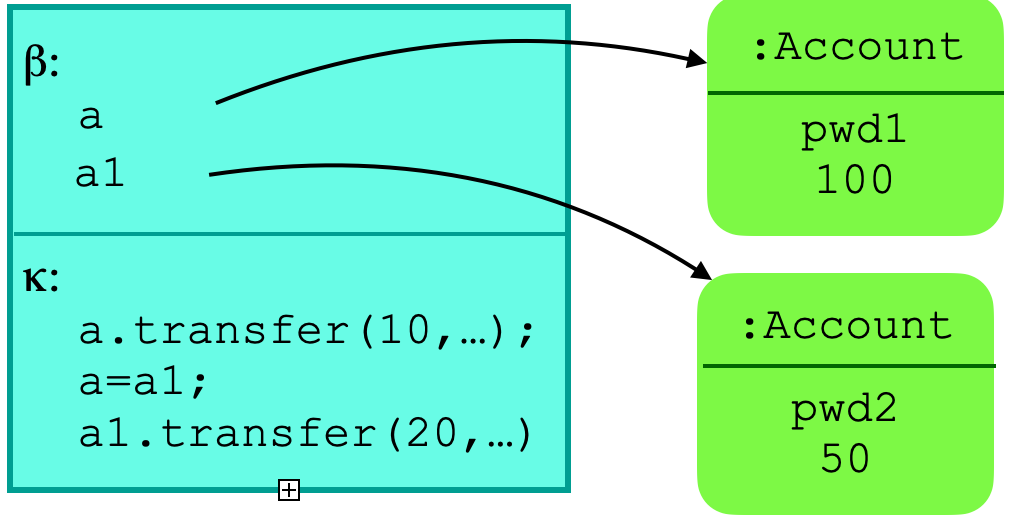
\includegraphics[width=\linewidth]{diagrams/adapt1.png}
%   \end{minipage}
% & \ \ \ &
% \begin{minipage}{0.27\textwidth}
%  $\sigma':$\\
% % ~ \ \\
%  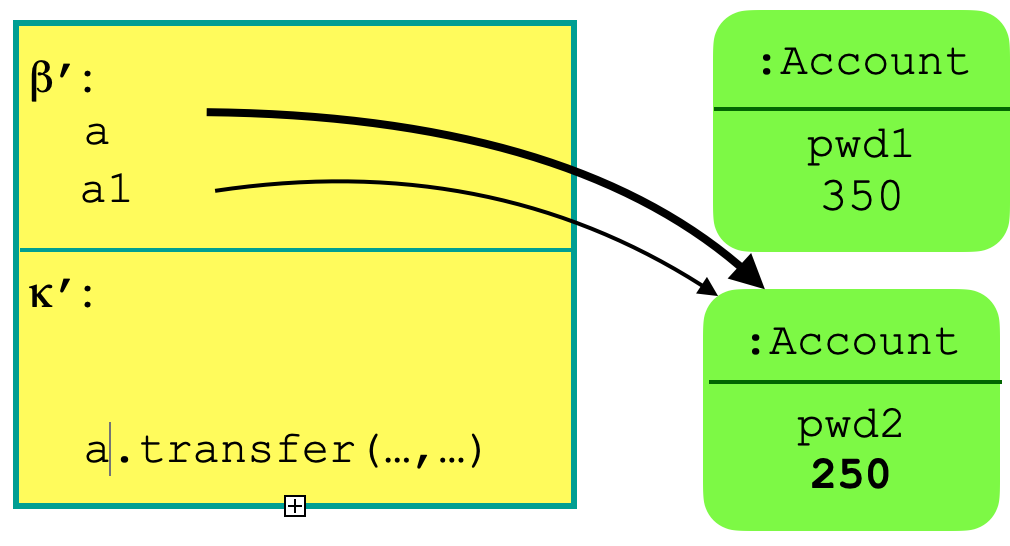
\includegraphics[width=\linewidth]{diagrams/adapt2.png}
%   \end{minipage}
%   & \ \ \  &
%    \begin{minipage}{0.27\textwidth}
%$\adapt {\sigma'}{\sigma}:$\\
%% ~ \\
%  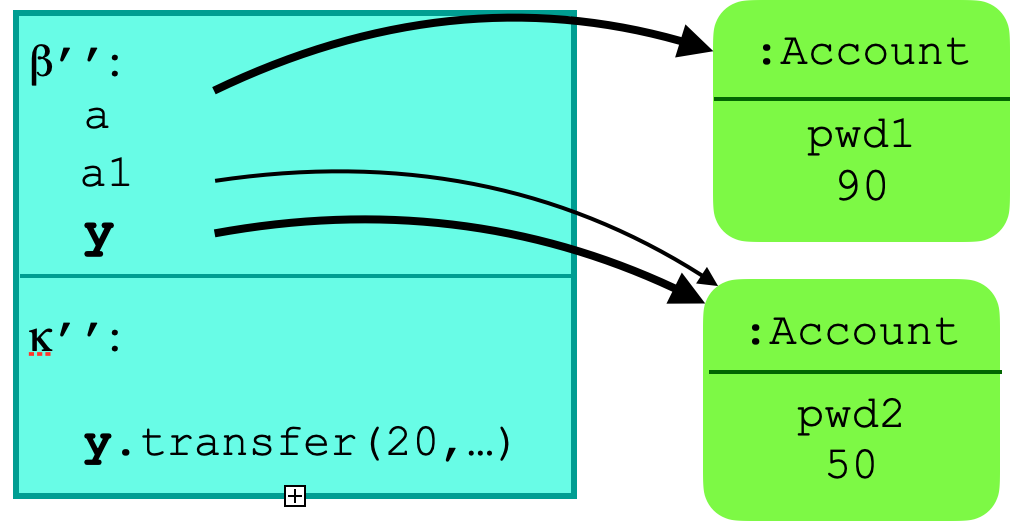
\includegraphics[width=\linewidth]{diagrams/adapt3.png}
%   \end{minipage}
%\end{tabular}
%\caption{Illustrating adaptation
%}
%\label{fig:Adaptation}
%\end{figure}
\newcommand{\mathsmall}[1]{\substack{\scalebox{0.8}{$#1$}}}
\begin{figure}[tbp]
\begin{tabular}{clclc}
 \begin{minipage}{0.27\textwidth}
 $\sigma:$\\
% ~ \\
 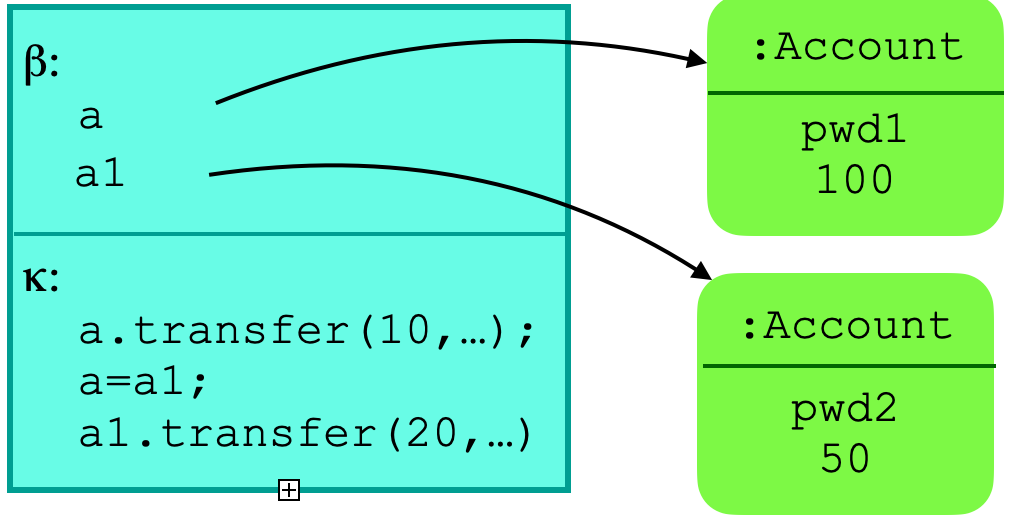
\includegraphics[width=\linewidth]{diagrams/adapt1.png}
   \end{minipage}
 & \ \ \ &
 \begin{minipage}{0.27\textwidth}
  $\sigma':$\\
 % ~ \ \\
  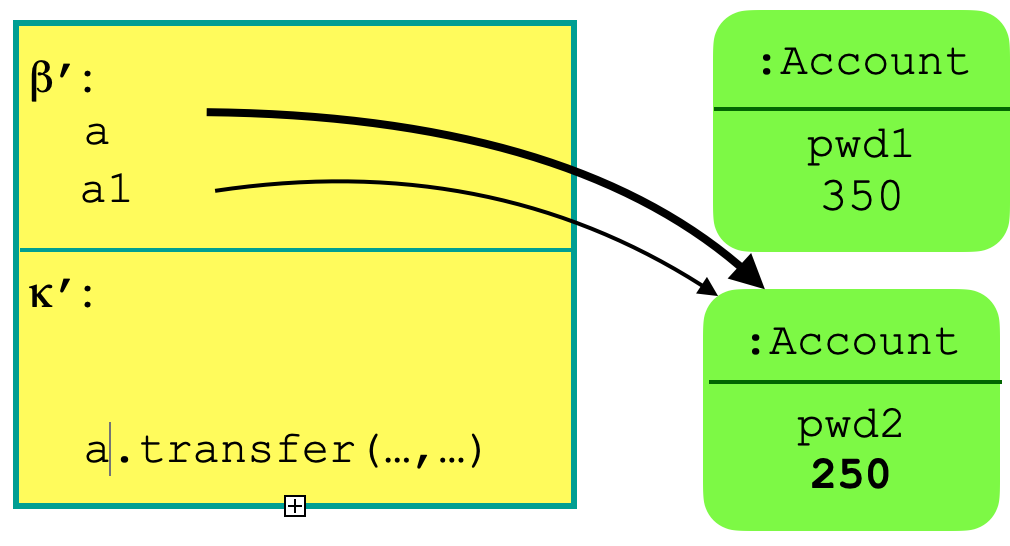
\includegraphics[width=\linewidth]{diagrams/adapt2.png}
   \end{minipage}
   & \ \ \  &
    \begin{minipage}{0.27\textwidth}
$\adapt {\sigma'}{\sigma}:$\\
% ~ \\
  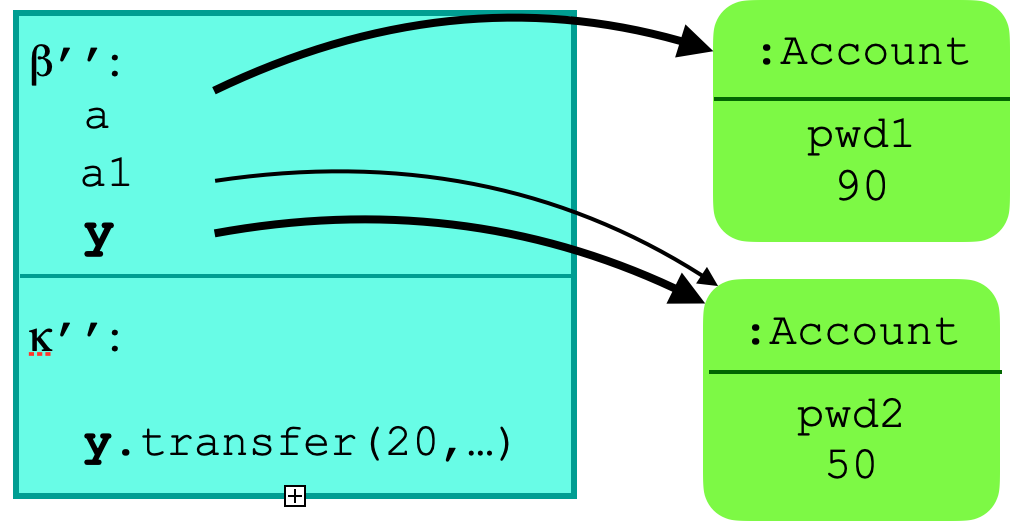
\includegraphics[width=\linewidth]{diagrams/adapt3.png}
   \end{minipage}
\end{tabular}

%\begin{tikzpicture}[->,>=to,shorten >=1pt,auto,node distance=5.5mm,
%                    thick,
%                    state/.style={circle,draw,minimum size=7mm,font=\sffamily\bfseries, color=hotpink, fill = hotpink, text = black, fill opacity = 0.5, scale=0.9},
%                    dots/.style={
%                    minimum size=7mm,
%                    font=\sffamily\Large\bfseries, 
%                    color=lightseagreen, 
%                    text = black, 
%                    fill opacity = 0.5},
%                    space/.style={
%                    minimum size=7mm,
%                    font=\sffamily\Large\bfseries, 
%                    color=lightseagreen, 
%                    text = black, 
%                    fill opacity = 0.5},
%                    arrow/.style={
%                    minimum size=7mm,
%                    font=\sffamily\Large\bfseries, 
%                    color=lightseagreen, 
%                    text = black, 
%                    fill opacity = 0.5},
%                    models/.style={
%                    minimum size=7mm,
%                    font=\sffamily\Large\bfseries, 
%                    color=lightseagreen, 
%                    text = black, 
%                    fill opacity = 0.5},
%                    decoration = snake]
%    
%    \node[space] (s) at (0,0) {};
%	\node[state, label={270:$\mathsmall{\vDash A_1}$}] (a) at (3.85,0) {$\sigma_1$};
%%	\node[space] (b) [right = of a] {};
%	\node[state, label={270:{$\mathsmall{\vDash A_2}$}}] (c) [right = of a] {$\sigma_n$};
%	\draw [decorate, ->]
%	(a) -- (c);
%\end{tikzpicture}
\caption{Illustrating adaptation
}
\label{fig:Adaptation}
\end{figure}




Under adaptation, the semantics of \Sadapt is:\  if $..,\sigma \models \prg{a.balance==350}$,
and  $.., \sigma \leadsto^* \sigma'$ and $..., \boldsymbol{\adapt {\sigma'}{\sigma}} \models \prg{a.balance==250}$,
%then $\sigma_1$'s continuation starts with a call to 
then {some intermediate state's continuation must contain  a call to \prg{a.transfer}};
\sd{where,  all \sd{variables bound in the initial state, $\sigma$,}
have the same bindings in $\adapt {\sigma'}{\sigma}$.}
\jm[I didn't understand susan's comment on this paragraph: ``problem with primes'']{}
 
Fig.~\ref{fig:Adaptation} illustrates the semantics of $\adapt {\sigma'}{\sigma}$. In   $\sigma$ the variable \prg{a} points to an \prg{Account}
 with password \prg{pwd1}, and balance \prg{350};  the variable \prg{a1} points to an \prg{Account}
  with password \prg{pwd2}, and balance \prg{350}; and the continuation is \prg{a1.transfer(}$..,..$\prg{);} \prg{a=a1;}
\prg{a.transfer(}$..,..$\prg{);}. 
We reach $\sigma'$ by executing the first two statements from the continuation.
Thus,  ${\adapt {\sigma'}{\sigma}}\not\models \prg{a.balance==250}$.
Moreover, in $\adapt {\sigma'}{\sigma}$ we introduce the fresh variables \prg{y} and \prg{y1}, and replace \prg{a} and
\prg{a1} by \prg{y} and \prg{y1} in the continuation.
This gives that ${\adapt {\sigma'}{\sigma}} \models \calls {\_} {\prg{a1}} {\prg{transfer}} {...}$ and  ${\adapt {\sigma'}{\sigma}}\not\models \calls {\_} {\prg{a}} {\prg{transfer}} {...}$.

 

Definition~\ref{d:adapt} \sd{describes} the $\adapt{}{}$ operator in all detail
(it is equivalent to, but not identical to the definition  given in \cite{FASE}).
We introduce fresh variables  $\overline{y}$ -- as many as in the $\sigma'$ top frame variable map
-- $dom(\beta')=\overline{x}$,  and $|\overline{y}| = |\overline{x}|$.  
We extend $\sigma$'s variable map ($\beta$), so that it also maps $\overline{y}$ 
in the way that  $\sigma'$'s variable map ($\beta'$) maps its local variables -- $\beta'' =  \beta[\overline{y} \mapsto  {\beta'(\overline{x})}]$. We rename $\overline{x}$   in $\sigma'$ continuation
to $\overline{y}$ --  $\kappa''=[\overline{y}/\overline{x}]\kappa'$.

 
 
\begin{definition}
\label{d:adapt}
For any states $\sigma$, $\sigma'$, heaps $\chi$, $\chi'$, %frames $\phi$, $\phi'$, 
variable maps $\beta$, $\beta'$, 
and continuations $\kappa$, $\kappa'$, such that 
$\sigma$=$(\chi,(\beta,\kappa):\psi)$, and $\sigma$=$(\chi',(\beta',\kappa'):\psi')$, we define  
\\
$\strut \ \ \ \ \bullet$  $\adapt{\sigma'}{\sigma} \triangleq (\chi', (\beta'',\kappa'') : \psi')$  
\\
where there exist variables $\overline{y}$ such that \ \ $\beta'' =  \beta[\overline{y} \mapsto  {\beta'(\overline{x})}]$, \ and\  $\kappa''=[\overline{y}/\overline{x}]\kappa'$, and 
%\item
$dom(\beta')=\overline{x}$,  and $|\overline{y}| = |\overline{x}|$,\  and\  $\overline{y}$ are fresh in $\beta$ and $\beta'$.
% \end{itemize}
%\end{itemize}
\end{definition}

Strictly speaking, $\adapt {}{}$  does not define one  unique state: Because  variables $\overline{y}$ 
are arbitrarily chosen,   $\adapt {}{}$ describes an infinite set of states. These states satisfy the same assertions
and therefore are   equivalent with each 
other.
This is why it is sound to  use $\adapt {}{}$  as an operator, rather than as a set.
 




\subsection{Expressiveness}

We discuss expressiveness of \Nec operators, by comparing 
them with one another, with temporal operators, and with other examples from the literature.

\paragraph{Relationship between Necessity Operators}
The three \Nec \ operators
are related by generality. 
%An 
 \emph{Only If} ($\onlyIf{A_1}{A_2}{A}$) implies
  \emph{Single-Step Only If} ($\onlyIfSingle{A_1}{A_2}{A}$), since if $A$ is 
a necessary precondition for multiple steps, then it must be a necessary 
precondition for a single step. 
 \emph{Only If} also implies 
an \emph{Only Through}, where the intermediate state is the starting state
of the execution.  There is no further relationship between 
\emph{Single-Step Only If} and \emph{Only Through}.


\paragraph{Relationship with Temporal Logic}
Two of the three \Nec operators can be expressed in traditional
  temporal logic: 
  ${\onlyIf{A_1}{A_2}{A}}$
can be expressed  %%put in to get better line breaks
 as 
 $A_1\ \wedge\ \Diamond A_2\ \longrightarrow\ A$, and
 $\onlyIfSingle{A_1}{A_2}{A}$
can be expressed  %%put in to get better line breaks
 as $\ A_1\ \wedge\ \bigcirc A_2\ \longrightarrow\ A$
 (where $\Diamond$ denotes any future state,  and
 $\bigcirc$ denotes the next state).
 Critically, 
$\onlyThrough{A_1}{A_2}{A}$ cannot be encoded in temporal logics
  without ``nominals'' (explicit state references), because the state where $A$ 
 holds must be between the state where $A_1$ holds, and the state
 where $A_2$ holds; and this must be so on \emph{every} execution path
 from $A_1$ to  $A_2$ \cite{hybridLogic2021,nominal-seplogic2020}.
 TLA+, for example, cannot describe ``only through'' conditions
 \cite{tlabook}, but we have found ``only through'' conditions critical
 to our proofs. 


% \subsection{More Examples expressed in \Nec}
% do not say \Nec Specifications
% because it is language that is expressive, not the specification
\label{s:expressiveness}

% \sdfootnote{  SD chopped the below -- some of it had moved to earlier, rest perhaps not that illuminating
%
%In this section we introduce some further specification examples, and use them to elucidate finer points
%in the semantics of \Nec. % We also  discuss which modules    satisfy  which specifications.
%
% \subsubsection{More examples of the Bank}
%Looking back at the examples from  \S\ref{s:bankSpecEx},   it holds that
%%\\
%%\strut $\hspace{.2in}$  \ModA$\vDash$ \SrobustA    $\hspace{.6in}$ \ModB$\vDash$ \SrobustA
%%  $\hspace{.6in}$ \ModC$\vDash$ \SrobustA
%%  \\
%%\strut   $\hspace{.2in}$  \ModA$\vDash$ \SrobustB    $\hspace{.6in}$ \ModB$\nvDash$ \SrobustB
%%  $\hspace{.6in}$ \ModC$\vDash$ \SrobustB
%  \\
%  $\begin{array}{llll}
%  \ \  \ \ \ \ \ & \ModA \vDash  \SrobustA    \ \ \ \ \ \ & \ModB \vDash \SrobustA \ \ \ \ \ \
%  &  \ModC \vDash \SrobustA
%  \\
% &  \ModA \vDash  \SrobustB    \ \ \ \ \ & \ModB \nvDash \SrobustB \ \ \ \ \ 
%  &  \ModC \vDash \SrobustB
%  \end{array}$
% 
%
% 
%Consider now another four \Nec specifications:
% 
%\begin{lstlisting}[language = Chainmail, mathescape=true, frame=lines]
%     $\text{\SRobustNextAcc}$   $\triangleq$  from a:Account $\wedge$ a.balance==bal  next a.balance < bal
%                        onlyIf $\exists$ o.[$\external{\texttt{o}}$ $\wedge$ $\access{\prg{o}}{\prg{a.pwd}}$]                                           
%
%     $\text{\SRobustNextCall}$  $\triangleq$  from a:Account $\wedge$ a.balance==bal  next a.balance < bal
%                        onlyIf $\exists$ o.[$\external{\texttt{o}}$ $\wedge$ $\calls{\prg{o}}{\prg{a}}{\prg{transfer}}{\prg{\_, \_, \_}}$]
%                       
%     $\text{\SRobustToCall}$   $\triangleq$  from a:Account $\wedge$ a.balance==bal to a.balance < bal
%                        onlyIf $\exists$ o.[$\external{\texttt{o}}$ $\wedge$ $\calls{\prg{o}}{\prg{a}}{\prg{transfer}}{\prg{\_, \_, \_}}$]  
%                                          
%     $\text{\SRobustThroughCall}$  $\triangleq$  from a:Account $\wedge$ a.balance==bal to a.balance < bal
%                       onlyThrough $\exists$ o.[$\external{\texttt{o}}$ $\wedge$ $\calls{\prg{o}}{\prg{a}}{\prg{transfer}}{\prg{\_, \_, \_}}$]
%
%\end{lstlisting}
%
%
%{The specification \SRobustNextAcc  states that
%the balance of an account decreases \emph{in one step}, only if an external object has access to the 
%password. It a weaker specification than \SrobustB, because it applies when the 
%decrease   takes place in \emph{one} step, rather than in \emph{a number} of steps.}
%Even though \ModB does not satisfy \SrobustB, it does satisfy \SRobustNextAcc:
% 
%  $\begin{array}{llll}
%  \   & \ModA \vDash \SRobustNextAcc  \   & \ModB \vDash \SRobustNextAcc \  
%  & \ModC \vDash \SRobustNextAcc \\
%  
%  \end{array}$
%
%\vspace{.07in} % SD thinks some space is needed here
%
%The specifications \SRobustNextCall and   \SRobustToCall are similar:
%they both say that a decrease of the balance can only happen if the current statement is a call to \prg{transfer}.  
%The former considers   a \emph{single} step, while the latter allows for \emph{any number} of steps. 
% \SrobustB is slightly different, because it  says that such a decrease is only possible if some \emph{intermediate}
% step called \prg{transfer}.
% All three   modules satisfy  \SRobustNextCall.  
%On the other hand, the code \prg{a1=new Account; a2.transfer}$(...)$ decrements the balance of \prg{a2} and
%does call \prg{transfer} but not as a first step; therefore, none of the modules satisfy 
%\SRobustToCall. That is:
%
%
% $\begin{array}{llll}
%  & \ModA \vDash \SRobustNextCall     & \ModB \vDash \SRobustNextCall   
%  & \ModC \vDash \SRobustNextCall
%  \\
%  & \ModA \nvDash \SRobustToCall     & \ModB \nvDash \SRobustToCall  
%  & \ModC \nvDash \SRobustToCall
%  \end{array}$
%  
%  \vspace{.07in} % SD thinks some space is needed here
%
% Finally, \SRobustThroughCall is a weaker requirement than \SRobustToCall, because it only asks
%  that the \prg{transfer} method is called in \emph{some intermediate} step. 
%  All modules satisfy it:
% 
% 
%   $\begin{array}{llll}
%  & \ModA \vDash\SRobustThroughCall     & \ModB \vDash \SRobustThroughCall  
%  & \ModC \vDash \SRobustThroughCall
%   \end{array}$
%
%}




\paragraph{The DOM}  %\sophiaPonder[renamed Wrapper to Proxy]{  
\label{ss:DOM}
This is the motivating example in \cite{dd},
dealing with a tree of DOM nodes: Access to a DOM node
gives access to all its \prg{parent} and \prg{children} nodes, with the ability to
modify the node's \prg{property} -- where  \prg{parent}, \prg{children} and \prg{property}
are fields in class \prg{Node}. Since the top nodes of the tree
usually contain privileged information, while the lower nodes contain
less crucial third-party information, we must be able to limit 
 access given to third parties to only the lower part of the DOM tree. We do this through a \prg{Proxy} class, which has a field \prg{node} pointing to a \prg{Node}, and a field \prg{height}, which restricts the range of \prg{Node}s which may be modified through the use of the particular \prg{Proxy}. Namely, when you hold a \prg{Proxy}  you can modify the \prg{property} of all the descendants of the    \prg{height}-th ancestors of the \prg{node} of that particular \prg{Proxy}.  We say that
\prg{pr} has \emph{modification-capabilities} on \prg{nd}, where \prg{pr} is
a  \prg{Proxy} and \prg{nd} is a \prg{Node}, if the \prg{pr.height}-th  \prg{parent}
of the node at \prg{pr.node} is an ancestor of \prg{nd}.
%}


The specification \prg{DOMSpec} states that the \prg{property} of a node can only change if
some external object presently has 
access to a node of the DOM tree, or to some \prg{Proxy} with modification-capabilties
to the node that was modified.
\begin{lstlisting}[language = Chainmail, mathescape=true, frame=lines]
DOMSpec $\triangleq$ from nd : Node $\wedge$ nd.property = p  to nd.property != p
          onlyIf $\exists$ o.[ $\external {\prg{o}}$ $\wedge$ 
                       $( \  \exists$ nd':Node.[ $\access{\prg{o}}{\prg{nd'}}$ ]  $\vee$ 
                         $\exists$ pr:Proxy,k:$\mathbb{N}$.[$\, \access{\prg{o}}{\prg{pr}}$ $\wedge$ nd.parent$^{\prg{k}}$=pr.node.parent$^{\prg{pr.height}}$ ] $\,$ ) $\,$ ]
\end{lstlisting}

\paragraph{More examples}
%or {\sc{VerX}}. 
% Nevertheless, 
%we believe that
%it  is powerful enough for the purpose of straightforwardly
%expressing robustness requirements. 
In order to investigate \Nec's expressiveness,  
we used it for
examples provided in the literature. 
% In this section we considered the DOM, %  example, proposed by  \citeasnoun{dd}. 
In \jm[]{the appendices of the full paper \cite{necessityFull}} % Appendix \ref{s:expressiveness:appendix},
we compare with examples proposed by  \citeasnoun{FASE}, and \citeasnoun{VerX}.
 



{We will now develop an inference system to prove that a module % is well-formed $\vdash M$, \ie that a module 
satisfies its specification. This is done in three phases.
%\TODO{\red{TODO: refer to what we said in approach section}}

%In the first phase, 
\textit{First Phase:} We develop a logic of triples ${\hproves{M}  {A} {\ stmt\ }{A'} }$,  with % which have 
the expected meaning, \ie 
(*) execution of statement $stmt$ in a state satisfying {the \emph{precondition}}  $A$ will lead to a state satisfying  {the \emph{postcondition}}  $A'$.
These triples only apply to   $stmt$'s  that  do not contain method calls  (even internal) -- this is so, because method calls may contain calls to external methods, and therefore can only be described through quadruples.
Our triples extend an underlying Hoare logic  (${M \vdash_{ul}  \{A\} {\ stmt\ } \{A'\} }$) and  introduce new judgements to %  which 
talk about protection.

\textit{Second Phase:} We develop a logic of quadruples ${\hprovesN{M}  {A} {\ stmt\ }{A'} {A''}}$. These promise,  that (*) and  
in addition,   that (**) any intermediate external states reachable during execution of that statement % will
 satisfy the invariant  $A''$.  
% {We call $A''$ the \midcond.}
 We incorporate all triples from the first phase,       
introduce invariants, give the usual substructural rules, and deal with method calls. 
For internal   calls we use the methods' specs. %, and in addition, for public methods we use the fact that they preserve the module's invariants. 
For external   calls, we   use %can only use  the fact that they preserve
 the module's invariants. 
 
\textit{Third Phase:} We prove modules' adherences to  specifications. 
For method specifications we prove that the body maps the precondition to the postcondition and preserves the method's invariant. 
For module invariants we prove that they  are preserved by the public methods of the module.



\paragraph{Preliminaries: Specification Lookup,  Renamings, Underlying Hoare Logic}

% Before describing the three phases, we  start with some preliminaries.
First some preliminaries: % shorter 
The judgement    $\promises M S$ expresses that $S$ is part of $M$'s specification.  
In particular, it allows   \emph{safe  renamings}. 
These renamings are   a convenience, akin to the Barendregt convention, and  allow simpler Hoare rules  -- \cf Sect. \ref{sect:wf},
Def. \ref{d:promises}, and Ex. \ref{e:rename}. We also require an underlying Hoare logic with judgements $M \vdash_{ul} \{ A \} stmt \{ A' \}$, 
% with  $\Stable{A}$,  $\Stable{A'}$ 
-- \cf Ax. \ref{ax:ul}.



\subsection{First Phase: Triples}

In  Fig. \ref{f:underly}  we introduce our triples, of the form ${   \hproves{M}  {A} {stmt}  {A'}}$. 
These promise, as expected, that any execution of $stmt$ in a state   satisfying $A$ leads to a state satisfying $A'$.
% chopped; we say it later in the lemma
%These triples only apply to statements that do not contain method calls.

{\small{
\begin{figure}[tht]
$
\begin{array}{c}
\begin{array}{lcl}
\inferruleSD{\hspace{0.5cm} [\sc{embed\_ul}]}
	{stmt  \ \mbox{contains no method call}   
        \\
        \Stable{A}  \ \  \Stable{A'}  \ \ \ \ \ \ \ \ \ \ { M \vdash_{ul} \{ \ A\ \} {\ stmt\ }\{\ A'\ \}}
	 	 }
	{\hproves{M}  {A} {\ stmt\ }{A'} } 
& &
\inferruleSD{\hspace{0.5cm} [\sc{prot-new}]}
	{
	\sdN{u \txtneq   x	 }
	}
	{	 
 	\hproves{M} 
 						{ \sdN{true} }  
 					{\  u = \prg{new}\ C \ }
 						  {  \inside{u}\  \wedge  \protectedFrom{u}{x}} 
 	} 
\\ \\
	{\inferruleSD{\hspace{0.5cm} [\sc{prot-1}]}
	{   stmt \ \mbox{ is free of  method cals, or assignment to $z$}
	\\
	{\hproves{M}  {{A \wedge} \re\!=\!z} {\ stmt\ }{ \re\!=\!z} }
	}
	{\hproves{M} 
						{\  {A \wedge} \inside{\re}  \ }
						{\  stmt \ }
						{\  \inside{\re}\ }
	}
}
& &
      {\inferruleSD{\hspace{0.5cm} [\sc{prot-2}]}
	{ stmt \mbox{ is either $x:=y$ or $x:=y.f$}\ \ \ \ \    z,z' \txtneq x 
		\\
	{\hproves{M} 
						{  {A \wedge} z\!=\!\re \wedge z'\!\!=\!\! \re' }
						{\ stmt }
						{   z\!=\! \re \wedge z'\!\!=\!\! \re' }
	}
	}
	{
	\hproves{M} 
						{\ {A \wedge} \protectedFrom{\re}{\re'}\ }
						{\ stmt }
						{\ \protectedFrom{\re}{\re'}\ }
	}
}
\\ \\
      {\inferruleSD{\hspace{0.5cm} [\sc{prot-3}]}
	{\sdN{x \txtneq   z	 } }
	{\hproves{M} 
						{\ \protectedFrom{y.f}{z}\ }
						{\ x =y.f\ }
						{\ \protectedFrom{x}{z}\ }
	}
}
& &
        {\inferruleSD{\hspace{0.5cm} [\sc{prot-4}]}
	{ }
	{\hproves{M} 
						{\ \protectedFrom{x}{z} \ \wedge \   \protectedFrom{x}{y'} }
						{\ y.f=y'\ }
						{\ \protectedFrom{x}{z} \ }
	}
}
\end{array}
\end{array}
 $
\caption{Embedding the Underlying Hoare Logic, and Protection}
\label{f:protection}
\label{f:underly}
\end{figure}
}}


With rule {\sc{embed\_u}} in Fig. \ref{f:underly},  any assertion $M \vdash_{ul} \{ A \} stmt \{ A' \}$  whose statement does not contain a method call, and which 
can be proven in the underlying Hoare logic, can also be proven in our logic. %More in \ref{s:types}.
In \textsc{Prot-1}, we see that  protection of an object $o$ is preserved by internal code which does not call any methods: namely any heap modifications will
ony affect internal objects, and this will not expose new, unmitigated external access to $o$.
%In \textsc{Prot-2}, the assignment $y=y'.f$ does not create a new route from $z$ to $x$, and therefore  $\protectedFrom{x}{z}$ is preserved.
 \textsc{Prot-2}, \textsc{Prot-3} and \textsc{Prot-4} describe the preservation of relative protection.
Proofs of these rules can be found in App. \ref{s:app:protect:lemmas}. 
% if $y.f$ is protected from some $z$, then the field access $x=y.f$ retains that protection, and therefore $\protectedFrom{x}{z}$.}
%In \textsc{Prot-4}, if $x$ is protected from $y'$, then the assignment $y.f=y'$ does not create a new unprotected route  to $x$, and therefore   $\protectedFrom{x}{z}$ is preserved.

Note that \se{the only way that}``protection'' of an object can decrease is if we call an external method, and pass it % not only internal 
an internal object 
 as argument. This will be  covered by the rule in Fig. \ref{f:external:calls}.
% \jm{Moreover, we introduce some consequence rules in \susan{Fig. \ref{f:protection}} to reason about protection apart from a Hoare logic. These are primarily useful when applying \textsc{Consquence} style Hoare rules.} 



\begin{lemma}
\label{l:no:meth:calls}
If ${\hproves{M}  {A} {\ stmt\ }{A'} }$, then $stmt$ contains no method calls.
\end{lemma}
  
%\jm{Fig. \ref{f:protection} extends an assumed underlying Hoare logic with rules for reasoning about protection. To supplement this, we introduce some consequence rules in Fig. \ref{f:protection:conseq} to reason about protection apart from a Hoare logic. These are primarily useful when applying \textsc{Consquence} style Hoare rules.}


%\begin{figure}[htb]
%\begin{mathpar}
%%\inferrule
%%	{M \vdash x : \prg{int} \rightarrow \protectedFrom{y}{x} }
%%	{}
%%	\quad[\textsc{Prot-Int}_1]
%%	\and
%%\inferrule
%%	{M \vdash x : \prg{int} \rightarrow \neg \protectedFrom{x}{y}}
%%	{}
%%	\quad[\textsc{Prot-Int}_2]
%%	\and
%%\inferrule
%%	{M \vdash x : \prg{bool} \rightarrow \protectedFrom{y}{x} }
%%	{}
%%	\quad[\textsc{Prot-Bool}_1]
%%	\and
%%\inferrule
%%	{M \vdash x : \prg{bool} \rightarrow \neg \protectedFrom{x}{y}}
%%	{}
%%	\quad[\textsc{Prot-Bool}_2]
%%	\and
%%\inferrule
%%	{M \vdash x : \prg{str} \rightarrow \protectedFrom{y}{x} }
%%	{}
%%	\quad[\textsc{Prot-Str}_1]
%%	\and
%\inferrule
%	{C \in M}
%	{M \vdash x : C \rightarrow x : \prg{intl}}
%	\quad[\textsc{Intl-M}]
%	\and
%\inferrule
%	{M \vdash x \neq y \wedge y : \prg{intl} \rightarrow \protectedFrom{x}{y}}
%	{}
%	\quad[\textsc{Prot-Intl}]
%\end{mathpar}
%\caption{Consequence Rules for Protection}
%\label{f:protection:conseq}
%\end{figure}

%\jm{Julian: I added the above, but these are not sensible with the current definition of protection because protection is only defined between objects, and not ints, bools, and strings. They are necessary for the example proofs (or alternatively we can use object encodings of these types, but I think that might be more difficult). The rules for strings are potentially not necessary. They only help make the Seciton 2 example work when we send back a message as a string. Similarly, we could probably drop the bool rules.}

\subsection{Second Phase: Quadruples}

\subsubsection{Introducing invariants, and substructural rules}
% Fig. \ref{f:substructural} 
We now introduce  quadruple rules. %  of the from ${\hprovesN{M}  {A} {\ s\ }{A'} {A''} }$. % which do not deal with method calls.
Rule {\sc{mid}} embeds  triples  ${\hproves{M}  {A} {\ s\ }{A'} }$  into quadruples ${\hprovesN{M}  {A} {\ s\ }{A'} {A''} }$; this is sound, because $s$ is guaranteed not to contain method calls (by lemma \ref{l:no:meth:calls})

\begin{center}
$
\begin{array}{c}
% \begin{array}{lcl}
\inferruleSD{[\sc{Mid}]}
	{\hproves{M}  {A} {\ s\ }{A'} }
	{\hprovesN{M}  {A} {\ s\ }{A'} {A''} }
  \end{array}
 $
 \end{center}
 
Substructural quadruple rules appear in  Fig. \ref{f:substructural:app}, and are as expected: 
Rules   {\sc{sequ}} and {\sc{consequ}} are  the usual rules for statement sequences and consequence, adapted to quadruples.
Rule {\sc{combine}} combines two quadruples for the same statement into one.
Rule  {\sc{Absurd}} allows us to deduce anything our of \prg{false} precondition, and  {\sc{Cases}} allows for case analysis.
These  rules  apply to \emph{any} statements -- even those containing method calls.

\subsubsection{Adaptation}

 \label{s:preserve:encaps}
 \label{s:viewAndProtect}
 
In the outline of the Hoare proof of the external call in  \S  \ref{sec:howThird},  we saw that an assertion of the form $\protectedFrom x {\overline {y}}$ at the call site,  may imply $\inside{x}$ at entry to the call.
More generally,  the $\pushSymbolInText$ operator  adapts an assertion from the view of the callee to that of the caller,
 and is used in the Hoare logic for method calls. It is defined below. 
 
 
\begin{definition}
\label{def:push}
[The $\pushSymbolInText$  operator]  

$
\begin{array}{c}
\begin{array}{l}
\begin{array}{rclcrcl}
  \PushAS y {\inside \re} & \triangleq &  \protectedFrom \re {\overline {y} }
  & \ \ \  \ &
  \PushAS y   {(A_1  \wedge  A_2)} & \triangleq &  (\PushAS y  { A_1})  \wedge  ( \PushAS y  {A_2} )  
\\ 
 \PushAS y {(\protectedFrom \re {\overline {u}})} &  \triangleq& \protectedFrom \re {\overline {u}} 
  & &
 \PushAS y  {(\forall x:C.A)} & \triangleq & \forall x:C.({\PushAS y A} )  
  \\  
  \PushAS y  {(\external \re)} &  \triangleq & {\external \re}  %   \PushAS y  {(\external \re)} & \triangleq &   {\external \re}
  & & 
  \PushAS y  {(\neg A)} &  \triangleq & \neg( {\PushAS y A} )  
    \\
     \PushAS y  {\re} &  \triangleq&   \re %    \PushAS y  {(\internal \re)} &  \triangleq & {\internal \re}
    & &
    \PushAS y  {(\re:C)} &  \triangleq&   \re:C 
 \end{array}
\end{array}
\end{array}
$
\label{f:Push}
\end{definition}
 

Only the first equation in  Def.  \ref{def:push}  is interesting: for $\re$ to be {protected at  a} callee with arguments $\overline y$, it should be protected from   % the call's 
these arguments -- thus
  $\PushAS y {\inside \re} = \protectedFrom {\re} {\overline {y}}$. 
The notation $\protectedFrom {\re} {\overline {y}}$   stands for $\protectedFrom \re {y_0}\  \wedge\  ...  \wedge \protectedFrom \re {y_n}$, assuming that $\overline y$=${y_0, ... y_n}$.

Lemma \ref{lemma:push:ass:state}  states that   
indeed, $\pushSymbolInText$ adapts assertions from the callee to the caller, and is the counterpart to the  
%operator 
$\pushSymbol$.
{In particular:\ \ 
 \ (\ref{l:push:stbl}):\    $\pushSymbolInText$ turns an assertion into a stable assertion.
\ (\ref{lemma:push:ass:state:one}):\ If the caller,   $\sigma$,  satisfies  $\PushSLong  {Rng(\phi)} {A}$, then  the callee,   ($\PushASLong {\phi} {\sigma}$), satisfies $A$.
\ \ (\ref{lemma:push:ass:state:two}): \ When returning from external states,  an assertion implies its adapted version.
 \ \ (\ref{lemma:push:ass:state:three}): \ When calling from external states, an assertion implies its adapted version. % (Lemma \ref{lemma:internal:adapted}).}
}
  

{
\begin{lemma} 
\label{lemma:push:ass:state}
For  states  $\sigma$, assertions $A$, %, $A'$  $Stb^+(A)$, and 
so that $Stb^+(A)$ and $\fv(A)=\emptyset$,  % with $\fv(A)=\emptyset$,  %variables   $\overline y$, 
frame $\phi$,  variables $y_0$, $\overline y$: % with $Range (\phi)=\overline {\interpret \sigma y}$:

\begin{enumerate}
 \item
\label{l:push:stbl}
$\Stable{\,  \PushASLong {(y_0,\overline y)} A\, }$
\item
 \label{lemma:push:ass:state:one}
$M, \sigma \models \PushASLong  {Rng(\phi)} {A}\ \  \ \ \ \ \  \ \ \    \Longrightarrow  \ \ \ \ M,  \PushSLong {\phi} {\sigma}   \models A$
\item
 \label{lemma:push:ass:state:two}
$M,  \PushSLong {\phi} {\sigma}   \models  A  \wedge \extThis    \ \  \ \ \  \  \Longrightarrow  \ \ \ \ M, \sigma \models \PushASLong  {Rng(\phi)} {A}$
 \item
 \label{lemma:push:ass:state:three}
$M, \sigma  \models  A  \wedge \extThis  \ \wedge \ M\cdot\Mtwo \models \PushSLong {\phi} {\sigma}   \ \  \ \ \  \  \Longrightarrow  \ \ \ \ M, \PushSLong {\phi} {\sigma} \models \PushASLong  {Rng(\phi)} {A}$
\end{enumerate}
\end{lemma}
}

{
Proofs %of the lemma can be found
 in \A\ \ref{appendix:adaptation}. Example \ref{push:does:not:imply}
 demonstrates the need for the   \prg{extl}  %  \prg{intl} and  
  requirement in  % (\ref{lemma:internal:adapted}) and 
  (\ref{lemma:push:ass:state:two}). %  above.  -- shorter
}



\begin{example}[When returning from   internal states, $A$ does not imply $\PushASLong {Rng(\phi} {A}$]  
\label{push:does:not:imply}   
In  Fig. \ref{fig:ProtectedBoth} we have
 $\sigma_2= \PushSLong {\phi_2} {\sigma_1}$, and    $\sigma_2 \models \inside{o_1}$,  and $o_1\in Rng(\phi_2)$.
But, since $o_1=o_1$, we also have  $\sigma_1 \not\models \protectedFrom {o_1} {o_1}$.
% not needed
%--   (\ref{lemma:push:ass:state:two}): \textit{When from popping internal states, $A$ does not imply $\PushASLong {Rng(\phi} {A}$}:\  We have $\sigma_2 \models \inside{o_1}$, 
%$o_1\in Rng(\phi_1)$But, since $o_1=o_1$, we do not have 
%$\sigma_2 \not\models \protectedFrom {o_1} {o_1}.$.
%
% needs checking
%--  \textit{$\PushASLong {Rng(\phi} {A}$ does not imply $A$}:\  In  $\sigma_2$ from Fig. we have $\sigma_1 \models \inside{o_1}$, and
%$o_1\in Rng(\phi_1)$. But, since $o_1=o_1$, we do not have 
%$\sigma_1 \not\models \protectedFrom {o_1} {o_1}$.  
%  where $\interpret {\sigma_1} {\prg{this}}$ = $o_1$, and $o_1$ is {external},  and there is no other object. Then, we have
%$\_,\sigma_1 \models \inside {\prg{this}}$ and $\_,\sigma_1 \not\models \protectedFrom {\prg{this}} {\prg{this}}$.
%\notesep Nor does  $\PushAS {y} {A}$  imply $A$.\  \Eg  take a $\sigma_2$ where $\interpret {\sigma_2} {\prg{this}}$ = $o_1$,
% $\interpret {\sigma_2} {x}$ = $o_2$ , and  $\interpret {\sigma_2} {x.f}$ = $o_3$, and $o_2$ is external, and there are no other objects or fields.
% Then $\_,\sigma_2 \models   \protectedFrom {x.f} {\prg{this}}$ but  $\_,\sigma_2 \not\models \inside {x.f}$.
% 
\end{example}






\subsubsection{Reasoning about   calls}
\label{s:calls}
is described in Fig. \ref{f:internal:calls}. {\sc{Call\_Int}}  %and {\sc{Call\_Int\_Adapt}}  
 for internal methods, whether public or private; \ % \  {\sc{Call\_Ext}} 
and {\sc{Call\_Ext\_Adapt}} and {\sc{Call\_Ext}\_Adapt\_Strong} for  external methods.




\begin{figure}[htb]
{\small{
$\begin{array}{c}
 \inferruleSD{\hspace{4.7cm} [\sc{Call\_Int}]}
	{
	   	\begin{array}{c}
		\promises  M {\mprepostN{A_1}{p\ C}{m}{x}{C}{A_2} {A_3}}  \\
		{A_1' = A_1[y_0,\overline y/\prg{this}, \overline x]  \ \ \ \ \ \ \ \ \  A_2' = A_2[y_0,\overline y,u/\prg{this}, \overline x,\prg{res}]}  
		          	\end{array}
		}
	{  \hprovesN {M} 
						{ \  y_0:C,\overline {y:C} \wedge  {A_1'}\ }  
						 { \ u:=y_0.m(y_1,.. y_n)\    }
					         { \ {A_2'} \ } 
						{  \ A_3 \ }  
}
% \\
%  \\
% removed, as not sound.The example in \refl{push:does:not:imply}   shows why not.
%{ \inferruleSD{\hspace{4.7cm} [\sc{Call\_Int\_Adapt}]}
%	{
%	   	\begin{array}{c}
%		\promises  M {\mprepostN{A_1}{p\ C}{m}{x}{C}{A_2} {A_3}}   \\
%				{A_1' = A_1[y_0,\overline y/\prg{this}, \overline x]  \ \ \ \ \ \ \ \ \  A_2' = A_2[y_0,\overline y,u/\prg{this}, \overline x,\prg{res}] }  
%
%          	\end{array}
%		}
%	{  \hprovesN {M} 
%						{ \,  y_0\!:\!C, \overline {y\!:\!C} \wedge {\PushASLong {{(y_0,\overline {y})}} {A_1'}}\ }
%												{ \, u\!:=\!y_0.m(y_1,.. y_n)\,    }
%						{ \  { \PushASLong  {{(y_0,\overline {y})}} {A_2'}  } \ }  
%						{  \  A_3\  }  
%}
%}
\\
 \\ 
 \inferruleSD{\hspace{4.7cm} [\sc{Call\_Ext}\_Adapt]}
 	{ 
	 \promises M   {\TwoStatesN {\overline {x:C}} {A}} 
        }
	{   \hprovesN{M} 
						{ \    { \external{y_0}} \,     \wedge \,  \overline{x:C}\  \wedge\ {\PushASLong {{(y_0,\overline {y})}}  {A}}  \ } 
						{ \ u:=y_0.m(y_1,.. y_n)\    }
						{ \   {\PushASLong {{(y_0,\overline {y})}}  A}  \ }
						{\  A \   }
	}	
\\
 \\ 
{
 \inferruleSD{\hspace{4.7cm} [\sc{Call\_Ext}\_Adapt\_Strong]}
 	{ 
	 \promises M   {\TwoStatesN {\overline {x:C}} {A}} 
        }
	{   \hprovesN{M} 
						{ \    { \external{y_0}} \,     \wedge \,  \overline{x:C}\ \wedge  A   \wedge\ {\PushASLong {{(y_0,\overline {y})}}  {A} }\  }   
						{ \ u:=y_0.m(y_1,.. y_n)\    }
						{ \   A \wedge {\PushASLong {{(y_0,\overline {y})}}  {A} } \  }  
						{\  A \   }	
}
}

\end{array}
$
}}
\caption{Hoare Quadruples for Internal and External Calls -- here $\overline y$ stands for $y_1, ... y_n$}
\label{f:internal:calls}
\label{f:external:calls}
\label{f:calls}
\end{figure}

For  internal calls, we  start, as usual,  by looking up the method's specification, and 
{substituting the formal  by the actual parameters parameters ($\prg{this}, \overline{x}$  by $y_0,\overline{y}$).} % in the method's pre- and post-condition.
  {\sc{Call\_Int}} is as expected:   we  require the precondition, and guarantee the postcondition and invariant.
%For {\sc{Call\_Int\_Adapt}} we require the adapted pre-condition ($  \PushASLong {(y_0, \overline y)}{A_1'}$  rather than $A_1'$) and also ensure the adapted post-condition ($ \PushASLong {(y_0, \overline y)}{A_2'}$  rather than $A_2'$).
%Remember that $ \PushASLong {(y_0, \overline y)}{A_1}$ at the caller's side guarantees that $A_1$ holds at the start of the call  (after pushing the frame with   $y_0, \overline y$), while  
%$A_2$ at the end of the call  guarantees that  $ \PushASLong {(y_0, \overline y)}{A_2}$  holds when returning to the caller's side  (after popping the callee's frame)
%-- cf.  lemma \ref{lemma:push:ass:state}.
 {\sc{Call\_Int}} %and {\sc{Call\_Int\_Adapt}}  are 
 {is} applicable whether the method is public or private.


For external calls, % {\sc{Call\_Ext\_Adapt}}, 
we consider the module's invariants. 
If the module promises to preserve $A$, \ie if  $\promises M   {\TwoStatesN {\overline {x:D}} {A}}$, {and  if its adapted version, $ \PushASLong {(y_0, \overline y)}{A}$},  holds before the call, then it also holds after  the call \ ({\sc{Call\_Ext\_Adapt}}).
{If, in addition, the un-adapted version also holds before the call, then it also holds after the call  ({\sc{Call\_Ext\_Adapt\_Strong}}).}
%\sdNew{We require the adapted invariant ($  \PushASLong {(y_0, \overline y)}{A}$  rather than $A$) and  ensure invariant (again $  \PushASLong {(y_0, \overline y)}{A}$  rather than $A$).
%Remember that $  \PushASLong {(y_0, \overline y)}{A}$ at the caller's side guarantees that $A$ holds at the start of the call  (after pushing the frame with   $y_0, \overline y$), and conversely, 
%$A\wedge \extThis$ at the end of the call  guarantees that  $ \PushASLong {(y_0, \overline y)}{A}$  holds when returning to the caller's side  (after popping the callee's frame)
%-- cf.  lemma \ref{lemma:push:ass:state}.
%}

% SHORTER
% Moreover, $A$ is also a \midcond of the call.


\vspace{.1cm}

Notice that %at the point of the call, 
  internal calls, {\sc{Call\_Int}}   require   the \emph{un-adapted} %version of the the 
 method  precondition (\ie $A_1'$), while   external calls, both {\sc{Call\_Ext\_Adapt}} and {\sc{Call\_Ext\_Adapt\_Strong}},  require the 
 \emph{adapted} % version of the 
 invariant (\ie $ \PushASLong {(y_0, \overline y)}{A}$). 
{This is sound, because  internal callees preserve  %variable-free, 
 $\Pos{\_}$-assertions} % are preserved against pushing of frames 
 -- \cf Lemma \ref{l:preserve:asrt}. 
On the other hand, %when the callee is external, then
% $\Pos{\_}$-assertions are not necessarily preserved against pushing of frames
 {external callees do not necessarily preserve  $\Pos{\_}$-assertions} -- \cf Ex. \ref{push:does:not:preserve}. 
Therefore, in order to guarantee that $A$ holds upon entry to the callee, we need to know that $ \PushASLong {(y_0, \overline y)}{A}$ held at the caller site -- \cf Lemma \ref{lemma:push:ass:state}.

% SD removed for time being:
%Remember also, that $A$ does not imply $ \PushASLong {(y_0, \overline y)} {A}$, nor does $ \PushASLong {(y_0, \overline y)}{A}$  imply $A$ -- \cf example \ref{push:does:not:imply}.


Remember that {popping frames does not necessarily preserve}
%SD droped below, as we say it also about 15 lines earlier 
% while $\Pos{\_}$,-assertions are preserved against pushing of internal frames, 
% above they 
 $\Pos{\_}$  assertions % are not necessarily preserved against popping of such frames 
-- \cf Ex. \ref{ex:pop:does:not:preserve}.
Nevertheless, {\sc{Call\_Int}} guarantees the unadapted version, $A$,  upon return from the call. 
This is sound, because of our % use  of the concept of
 \emph{\scoped satisfaction} of assertions -- more in Sect.  \ref{s:scoped:valid}.
 

%{Rules  {\sc{CallAndAlias}}  and  {\sc{CallNonAlias}} say that calls preserve aliasing, resp. non-aliasing, between variables, ie they preserve $x=x$ resp. $x\neq x$. These two rules apply to internal as well as external calls. When the callee's receiver is external, they make the extra requirement that  $\PushAS {y}{\extract{M}}$ -- we  will discuss this requirement together with the discussion of Fig. \ref{f:external:calls}.     Note that $x=x'$ expresses that $x$ and $x'$ are aliases, while  $u\txteq x$ expresses that $u$ and $x$ are textually the same --
%the latter is stronger, i.e.   $x\txteq u$ implies $x=u$. 
%% It is possible that variables are aliases, without being textually the same, i.e. it is possible to have $x=x'$ while $u\not\equiv x'$. 
% As $...\equiv ...$ is a textual assertion, and thus  state-independent,  it is a side-condition of the rules and is  not part of the Hoare triple's precondition.
%}
%
%
%\small{
%\begin{figure}[hbt]
%$\begin{array}{c}
%\inferruleSD{\hspace{4.7cm}  [{\sc{CallAndAlias}}}
%	{ 
%	{   x \txtneq u\txtneq x'  }
%	}
%	{   \hproves{M}  { \ x=x'\   \wedge \ ({\external{y_0}}  \rightarrow \  \PushAS {y}{\extract{M}})\  }	{ \ u:=y_0.m(y_1,.. y_n)\  } { \  x=x'\ }	 }
%
%\\ \\ 
%\inferruleSD{\hspace{4.7cm} [{\sc{CallNonAlias}}]}	
%{ 
%		{ \ x \txtneq u \txtneq x'\   }
%	}
%	{   \hproves{M}   { \ x\neq x'\   \wedge \ ({\external{y_0}}  \rightarrow \  \PushAS {y}{\extract{M}})\  } { \ u:=y_0.m(y_1,.. y_n))\  } { \  x\neq x'\ }	 }
%\\
%\\
%\end{array}
%$
%\caption{Logic for Aliasing around Calls }
%\label{f:internal:alias:calls}
%\end{figure}
%}

\paragraph{Discussion: Polymorphic Calls} Our rules do  not directly address the possibility that the receiver might belong to one class or another class, or
even be   internal or external, and
where the choice is made at runtime. 
However, such scenaria  can be  supported through the case-split rule and the rule of consequence. 
More details in h \A\  \ref{app:polymorphic}.

\begin{example}[Proving external calls]
We continue our discussion from \S \ref{sec:howThird} on how to establish the Hoare triple    \textbf{(1)} :

 \vspace{.05cm}
  \begin{minipage}{.05\textwidth}
   \textbf{(1?)}\ \ 
\end{minipage}
\hfill
\begin{minipage}{.95\textwidth}
\begin{flushleft}
$\{\  \   \external{\prg{buyer}} \ \wedge\ 
% red here is meanrt to make the contrast with the  next one 
   {\protectedFrom {\prg{this.\myAccount.key}}  {\prg{buyer} } }
 \ \wedge\ \prg{this.\myAccount.\balance}= b  \ \  \}$\\
$\ \ \ \ \ \ \ \ \ \ \ \ {\ \prg{buyer.pay(this.accnt,price)}   \ } $\\
$  \{\  \ \  {\prg{this.\myAccount.\balance}} \geq  b \  \  \} \ \ ||\ \  \{\ \inside{\prg{a.\password}}\wedge  \prg{a.\balance}\!\geq\!{\prg{b}}   \ \}  $ 
\end{flushleft}
\end{minipage}
 
\vspace{.03cm}
\noindent
We use $S_3$, which says that $\TwoStatesN{ \prg{a}:\prg{Account},\prg{b}:\prg{int} } {\inside{\prg{a.key}} \wedge \prg{a.\balance} \geq \prg{b} }$. 
We can apply rule {\sc{Call\_Ext\_Adapt}}, by taking  $y_0 \triangleq \prg{buyer}$,  and $\overline {x : D}\triangleq \prg{a}:\prg{Account},\prg{b}:\prg{int}$, 
and $A \triangleq  \inside{\prg{a.\pwd}}\wedge \prg{a.\balance}\geq \prg{b}$, \ \ 
and $m \triangleq \prg{pay}$,\ and $\overline {y} \triangleq \prg{this.accnt},\prg{price}$,
and provided that we can establish that\\
\strut \ \ \   \textbf{(2?)}  $ {\small{\strut \ \ \ \protectedFrom {\prg{this.\myAccount.key}} {(\prg{buyer},\prg{this.\myAccount},\prg{price})}}}$\\
holds. Using   Def. \ref{def:push}, and type information, we can indeed establish that\\
\strut \ \ \   \textbf{(3)} $ {\small{\strut \ \ \ \protectedFrom {\prg{this.\myAccount.key}} {(\prg{buyer},\prg{this.\myAccount},\prg{price})}  \ = \   \protectedFrom {\prg{this.\myAccount.key}} {\prg{buyer}}}}$\
Then, by application of the rule of consequence, \textbf{(3)}, and the rule {\sc{Call\_Ext\_Adapt}}, we can establish \textbf{(1)}.\ \ \ 
More details in \S  \ref{l:buy:sat}.
\end{example}

\subsection{Third phase: Proving adherence to Module Specifications}
\label{sect:wf}

In Fig. \ref{f:wf} we  define the judgment $\vdash M$, which says that  
$M$ has been proven to be well formed. 
 

\begin{figure}[thb]
$
\begin{array}{l}
\begin{array}{lcl}
\inferruleSDNarrow 
{~ \strut  {\sc{WellFrm\_Mod}}}
{  \vdash \SpecOf {M}
  \hspace{1.2cm}  M \vdash \SpecOf {M}
}
{
\vdash M  
}
& \hspace{0.7cm} &
\inferruleSDNarrow 
{~ \strut   {\sc{Comb\_Spec}}}
{  
M \vdash S_1 \hspace{1.2cm}  M \vdash S_2
}
{
M \vdash S_1 \wedge S_2
}
\end{array}
\\
\inferruleSD 
{~ \strut \hspace{6.5cm} {\sc{method}}}
{  
 \prg{mBody}(m,D,M)=p \ (\overline{y:D})\{\  stmt \ \}       
    \\
  {\hprovesN{M} { \ \prg{this}:\prg{D}, \overline{y:D}\, {\wedge\, A_1}\  } %\, \sdN{\wedge\, \PushASLong {(\prg{this},\overline y)}  {A_1}}\, } 
  {\ stmt\ } {\ A_2\, \sdN{\wedge\, \PushASLong {\prg{res}} {A_2}} \ }   {A_3} } 
}
{
M \vdash {\mprepostN {A_1}{p\ D}{m}{y}{D}{A_2} {A_3} }
}
\\
\inferruleSD 
{~ \strut \hspace{6.5cm} {\sc{invariant}}}
{
\begin{array}{l}
\forall  D,  m:\ \ \  \ \  \prg{mBody}(m,D,M)=\prg{public} \ (\overline{y:D})\{\  stmt \ \}      \ \ \Longrightarrow  
  \\
   ~ \strut \hspace{0.3cm}  \ \ \ 
 \begin{array}{l}
   \hprovesN {M}  
{ \ \prg{this}:\prg{D}, \overline{y:D},\,   \overline{x:C} \, \wedge\,  A \, \sdN{\wedge\, \PushASLong {(\prg{this},\overline y)} {A}}\, }  
  	{\ stmt\ }   
	 {\  A\, \wedge\, \PushASLong {\prg{res}} {A} \ }  
{\ A \ }
 \end{array}
 \end{array}
}
{
M \vdash \TwoStatesN{ \overline{x:C}} {A}
}
\end{array}
$
\caption{Methods' and Modules' Adherence to Specification}
\label{f:wf}
\end{figure}

\footnoteSD{Julian's reflections on the invariant and method call rules:

 I think it somewhat makes sense for the Invariant rule to be asymmetric since
calls to internal code are asymmetric from the perspective of protection. There is no change in specific protection when entering 
internal code, but there may be when returning to external code from internal code. 

I'd have to think about it more, but I don't believe there is any decrease in general protection when entering internal code,
but there may be when exiting internal code. The adaptation in the post-condition is there to address the potential
for protection to be lost on return.

Magic wand adaptation (i.e. A -* x) expresses what must hold before crossing the boundary from internal to external code
(i.e. before an internal method return or call to an external method) for the adapted assertion to still be satisfied after crossing 
that boundary. I think there are a few things that are useful to consider here:
it is good to note that if you remove protection from the assertion language, the magic wand would be the identity
(i.e. A -* x = A) since only protection is modified when passing values between objects via method calls
more importantly, the way we define protection is based around fields and external/internal objects, and passing a value
to an internal object (via a method call) modifies neither a field nor grants any external object access to any other object
According to my understanding of the intended semantics of the magic wand, entering internal code from frame should
not affect any sort of protection.
My impression is that part of the intent of the magic wand is to be able to express ``what needs to hold before a call
so that <x>  holds within the new frame (whether that frame is internal or external)?''. I still need to think about how that
fits in with my above description of magic wand adaptation.
}


{\sc{Method}} says that  
a module satisfies a method specification if the % choopped method body for space
body satisfies the corresponding pre-, post- and \midcond. 
% The following sentence is wrong!
%\sdN{Moreover, the precondition is strengthened by $\PushASLong {(\prg{this},\overline y)} {A}$ -- this is sound because the state is internal, and by Lemma  \ref{lemma:internal:adapted}.
 In  the postcondition we also ask that $\PushASLong {\prg{res}}  {A}$, so that \prg{res} does not leak any of the values that $A$ promises will be protected. 
{\sc{Invariant}} says that  a module satisfies {a} %an invariant 
specification $\TwoStatesN{ \overline{x:C}} {A}$,  if the method body of each public method
 has $A$ as its  pre-, post- and \midcond. 
{Moreover, the precondition is strengthened by $\PushASLong {(\prg{this},\overline y)} {A}$ -- this is sound because
 the caller is external, and by Lemma   \ref{lemma:push:ass:state}, part (\ref{lemma:push:ass:state:three}).}
 
 \vspace{.1cm}

\noindent
\textbf{Barendregt} In  {\sc{method}} we \sdN{implicitly} require   the free variables  in a method's precondition  not to overlap with variables in its body, unless they are the receiver or one of the parameters ($\sdN{\vs(stmt) \cap \fv(A_1) \subseteq   \{ \prg{this}, y_1, ... y_n \} }$).  And in {\sc{invariant}} we require   the free variables in $A$ (which are a subset of  $\overline x$) not to overlap with the variable  in $stmt$ ($ \sdN{ \vs(stmt)\,  \cap\, \overline x\, =\, \emptyset}$).
This can easily be achieved through renamings, \cf Def. \ref{d:promises}.

\newcommand{\sdsp}{\strut \ \ \ \ \ }

\begin{example}[Proving a public method] Consider the proof that \prg{Account::set} from $M_{fine}$ satisfies $S_2$. Applying rule {\sc{invariant}}, we need to establish:\\
{\small{ \vspace{.05cm}
  \begin{minipage}{.05\textwidth}
  \textbf{(5?)}\ \ 
\end{minipage}
\hfill
\begin{minipage}{.95\textwidth}
\begin{flushleft}
$\{ \  \   ... \prg{a}:\prg{Account}\ \wedge\,  {\inside{\prg{a.key}}} \, \wedge \, \protectedFrom {\prg{a.key}} {(\prg{key'},\prg{key''})} \  \} \ $\\
$\ \ \ \ \ \ \ \ \ \ \  \prg{body\_of\_set\_in\_Account\_in}\_ M_{fine}\   $\\
$  \{\  \ \   \{ {\inside{\prg{a.key}}}\ \wedge\ {\PushASLong {\prg{res}\ } {\ \inside{\prg{a.key}}}} \   \} \ \ \  || \ \ \ 
	   \{ {\inside{\prg{a.key}}} \}  $ 
\end{flushleft}
\end{minipage}
}}
\vspace{.03cm}
\noindent
Given the conditional statement in \prg{set}, and with the obvious treatment of conditionals (\cf Fig. \ref{f:substructural:app}), among other things, we  need to prove for the \prg{true}-branch that:\\
\vspace{.01cm}
{\small{  \begin{minipage}{.05\textwidth}
  \textbf{(6?)}\ \ 
\end{minipage}
\hfill
\begin{minipage}{.95\textwidth}
\begin{flushleft}
$\{ \  \   ...    {\inside{\prg{a.key}}} \, \wedge \, \protectedFrom {\prg{a.key}} {(\prg{key'},\prg{key''})}  \wedge  \,  \prg{this.key}=\prg{key'}\  \} \ $\\
$\ \ \ \ \ \ \ \ \ \ \  \prg{this.key := key'}\   $\\
$  \{\  \ \   \{ {\inside{\prg{a.key}}}\   \   \} \ \ \  || \ \ \   \{ {\inside{\prg{a.key}}} \}  $ 
\end{flushleft}
\end{minipage}
}}
\\
 \vspace{.03cm}
\noindent
We can apply case-split  (\cf Fig. \ref{f:substructural:app}) on whether \prg{this}=\prg{a}, and thus a proof of \textbf{(7?)} and \textbf{(8?)}, gives a proof of \textbf{(6)}:\\
 \vspace{.03cm}
{\small{  \begin{minipage}{.05\textwidth}
   \textbf{(7?)}\ \ 
\end{minipage}
\hfill
\begin{minipage}{.95\textwidth}
\begin{flushleft}
$\{ \  \   ...    {\inside{\prg{a.key}}} \, \wedge \, \protectedFrom {\prg{a.key}} {(\prg{key'},\prg{key''})} \wedge  \,  \prg{this.key}\!=\!\prg{key'}\ \wedge\ \prg{this}\!=\!\prg{a}  \} \ $\\
$\ \ \ \ \ \ \ \ \ \ \   \prg{this.key := key'}\    $\\
$  \{\  \ \   \{ {\inside{\prg{a.key}}}  \   \} \ \ \  || \ \ \     \{ {\inside{\prg{a.key}}} \}  $ 
\end{flushleft}
\end{minipage}
}}
\\
and also
\\
 \vspace{.03cm}
{\small{  \begin{minipage}{.05\textwidth}
   \textbf{(8?)}\ \ 
\end{minipage}
\hfill
\begin{minipage}{.95\textwidth}
\begin{flushleft}
$\{ \  \   ...   {\inside{\prg{a.key}}} \, \wedge \, \protectedFrom {\prg{a.key}} {(\prg{key'},\prg{key''})}  \wedge  \,  \prg{this.key}\!=\!\prg{key'}\ \wedge\ \prg{this}\!\neq\!\prg{a}  \} \ $\\
$\ \ \ \ \ \ \ \ \ \ \  \prg{this.key := key'}\   $\\
$  \{\  \ \   \{ {\inside{\prg{a.key}}}  \   \} \ \ \  || \ \ \     \{ {\inside{\prg{a.key}}} \}  $ 
\end{flushleft}
\end{minipage}
}}
\\
 \vspace{.03cm}
\noindent
If  $ \prg{this.key}\!=\!\prg{a'} \wedge\ \prg{this}\!=\!\prg{a}$, then $\prg{a.key}\!=\!\prg{key'}$; this  contradicts that $\protectedFrom {\prg{a.key}} {\prg{key'}}$. So,  by contradiction (\cf Fig. \ref{f:substructural:app}), we can prove    \textbf{(7?)}.
When  $\prg{this.key}\!\neq \!\prg{a}$, we  obtain from the underlying Hoare logic that the value of \prg{a.key} did not change. Thus, we can apply rule {\sc{Prot\_1}}, and obtain  \textbf{(7?)}. \ \ \ More details in \S \ref{l:set:sat}.
 
 \vspace{.045cm}
\noindent
On the other hand, \prg{set} from $M_{bad}$ cannot be proven to satisfy $S_3$. Namely, it % \prg{set} from $M_bad$ 
% does not have the condition \prg{this.key}=\prg{key'}, and 
would require  us to prove that\\
\vspace{.03cm}
{\small{  \begin{minipage}{.05\textwidth}
   \textbf{(??)}\ \ 
\end{minipage}
\hfill
\begin{minipage}{.95\textwidth}
\begin{flushleft}
$\{ \  \   ...    {\inside{\prg{a.key}}} \, \wedge \, \protectedFrom {\prg{a.key}} {(\prg{key'},\prg{key''})}  \   \} \ $\\
$\ \ \ \ \ \ \ \ \ \ \  \prg{this.key := key'}\   $\\
$  \{\  \ \   \{ {\inside{\prg{a.key}}}\   \   \} \ \ \  || \ \ \   \{ \ {\inside{\prg{a.key}}} \ \}  $ 
\end{flushleft}
\end{minipage}
}}
\\
and without the condition \prg{this.key}=\prg{key'} there is no way we can prove \textbf{(??)}.

\subsection{Our Example Proven} % of our proof system}
\label{sect:example:proof:short}
Using our Hoare logic, we have developed a mechanised proof in Coq, that, indeed, $M_{good} \vdash S_2 \wedge S_3$.
This proof is  part of the accompanying artifact. 
 
 Our proof models  \LangOO, the assertion language, the specification language, and the Hoare logic from \S \ref{s:hoare:first},  \S   \ref{s:hoare:second},  \S  \ref{sect:wf},  \S \aref{F}{\ref{app:hoare}} and Def. \ref{def:push}.
In keeping with   the start of  \S \ref{sect:proofSystem}, our proof assumes the existence of an underlying Hoare logic,  
and several, standard, properties of that underlying logic, the assertions logic (\eg equality of objects implies equality of field accesses) and of type systems
(\eg  fields of objects of different types cannot be aliases of one another).
All assumptions  are clearly indicated in the associated artifact.
 Appendix \aref{H}{\ref{s:app:example}}  %included in the auxiliary material, 
outlines   that proof. 

% Finally, we discuss why  $M_{good} \not\vdash S_2 $

\end{example}

 


\section{Proving that \ModC satisifes \SrobustB}
\label{s:examples}
We now revisit our example from  \S  \ref{s:intro} and \S \ref{s:outline},
and outline a proof that \ModC satisfies \SrobustB. 
A {summary} of this proof has already been discussed in \S \ref{s:approach}.
 A more complex variant of this example that employs   can be found in Appendix \ref{app:examples}.
 \sdN{It demonstrates dealing with modules consisting of several classes some of which are confined, and
 which use ghost fields
 defined through functions; it also demonstrates proofs of assertion encapsulation of assertions 
 which involve reading the values of 
 several fields.} \julian{Mechanised versions of the proofs in both this Section, and Appendix \ref{app:examples}
 can be found in the associated Coq artifact in \prg{simple\_bank\_account.v} and \prg{bank\_account.v} respectively.}
 
 \jm[todo: add reference so \prg{simple\_bank\_account.v} \& \prg{bank\_account.v}]{}
 
Recall that an \prg{Account} includes %a \prg{balance} field, and a \prg{transfer} method, along with any other fields and methods. 
 at least a  field  (or ghost field)  called \prg{balance}, and a method called \prg{transfer}. 

%
 We first rephrase 
\SrobustB to use the $\wrapped{\_}$ predicate.
\begin{lstlisting}[language=Chainmail, mathescape=true, frame=lines]
$\SrobustB$ $\triangleq$ from a:Account $\wedge$ a.balance=bal 
          to a.balance < bal onlyIf $\neg\wrapped{\prg{a.pwd}}$
\end{lstlisting}

We next revisit the   \funcSpec from \S \ref{s:bank} and derive the following 
\prg{PRE}- and \prg{POST}-conditions. The first two pairs of \prg{PRE}-, \prg{POST}-conditions correspond to the first two \prg{ENSURES}
clauses from \S \ref{s:bank}, while the next two pairs correspond to the \prg{MODIFIES}-clause. The current expression in terms
of \prg{PRE}- and \prg{POST}-conditions is weaker than the one in \S \ref{s:bank}, and is not modular, but is
sufficient for proving adherence to  \SrobustB.

\begin{lstlisting}[mathescape=true, frame=lines, language=Chainmail]
$\SclassicP$  $\triangleq$
   method transfer(dest:Account, pwd':Password) -> void  
      (PRE: this.balance$=$bal1 $\wedge$ dest.balance$=$bal2 $\wedge$ this.pwd$=$pwd' $\wedge$ this$\neq$dest
       POST: this.balance=bal1-100 $\wedge$ dest.balance=bal2+100)
      (PRE: this.balance$=$bal1 $\wedge$ dest.balance$=$bal2 $\wedge$ (this.pwd$\neq$pwd' $\vee$ this$=$dest)
       POST: this.balance=bal1 $\wedge$ dest.balance=bal2)
      (PRE: a:Account $\wedge$ a.balance$=$bal $\wedge$ a$\neq$this $\wedge$ a$\neq$dest 
       POST: a.balance=bal)          
      (PRE: a:Account $\wedge$ a.pwd$=$pwd1  
       POST: a.pwd=pwd1)         
\end{lstlisting}


%\begin{figure}[t]
%\begin{lstlisting}[mathescape=true, frame=lines]
%module $\ModC$
%  class Password{}
%  class Account
%    field balance:int
%    field pwd:Password
%    method set(pwd':Password, pwd'':Password):void
%      {if(this.pwd==pwd') 
%         this.pwd := pwd'}
%	method transfer(pwd':Password, destAcc:Account)
%	  {if(this.pwd==pwd' && this.balance > 100)
%	     this.balance := this.balance - 100
%	     destAcc.balance := destAcc.balance + 100}
%\end{lstlisting}
%\caption{Bank Account Module}
%\label{f:ex-bank-short1}
%\end{figure}

%Susan: I changed the label because somewhere (I think in an appendix) there is a f:ex-bank-short and the ref picks it up rather than this one

\subsection{Part 1: Assertion Encapsulation}
\label{s:BA-encap}
The first part of the proof demonstrates that the \prg{balance}, \prg{pwd}, and external accessibility to the password are 
encapsulated properties. That is, for the \prg{balance} to change (i.e. for \prg{a.balance = bal} to be invalidated), or for 
or for the encapsulation of \prg{a.pwd} to be broken (ie for a transition from ${\wrapped{\prg{a,pwd}}}$ to $\neg {\wrapped{\prg{a.pwd}}}$),
internal computation is required. 

We use \sdNr[used to say "a conservative approach to an encapsulation system" but "conservative" here means sound]{a simple encapsulation system}, detailed in \jm[]{Appendix} \ref{s:encap-proof}, 
and provide the proof steps below.
\textbf{\prg{aEnc}} and \textbf{\prg{balanceEnc}} state that 
\jm[]{\prg{a} and \prg{a.balance}} satisfy \sdN{the \textsc{Enc$_e$} predicate. That is, if any objects' contents are to be
looked up during execution of these expressions, then these objects are internal.}
\textsc{Enc}$_e$(\prg{a}) holds because no object's contents is looked up,
while \textsc{Enc}$_e$(\prg{a.balance}) holds because \prg{balance} is a field of \prg{a}, and \prg{a} is
internal.
\\
\begin{figure}[h]
\begin{proofexample}
\proofsteps{\prg{BalEncaps}}
	{\begin{proofexample}
		\proofsteps{\prg{aEnc}}
			{\proofstepwithrule
			{$\proves{\ModC}{\givenA{\prg{a:Account $\wedge$ a.balance=bal}}{\intrnl{\prg{a}}}}$}
				{by \textsc{Enc$_e$-Obj}}
		}
		\endproofsteps
	\end{proofexample}
		}
	{\begin{proofexample}
		\proofsteps{\prg{balanceEnc}}
			{\proofstepwithrule
			{$\proves{\ModC}{\givenA{\prg{a:Account $\wedge$ a.balance=bal}}{\intrnl{\prg{a.balance}}}}$}
				{by \prg{aEnc} and \textsc{Enc-Field}}
		}
		\endproofsteps
	\end{proofexample}
		}
	{\begin{proofexample}
		\proofsteps{\prg{balEnc}}
			{\proofstepwithrule
			{$\proves{\ModC}{\givenA{\prg{a:Account $\wedge$ a.balance=bal}}{\intrnl{\prg{bal}}}}$}
				{by \textsc{Enc$_e$-Int}}
		}
		\endproofsteps
	\end{proofexample}
		}
		{\proofstepwithrule
			{
			$\proves{\ModC}{\givenA{\prg{a:Account $\wedge$ a.balance=bal}}{\encaps{\prg{a.balance=bal}}}}$
			}{by \prg{balanceEnc}, \prg{balEnc}, \textsc{Enc-Eq}, and \textsc{Enc-=}}}
\endproofsteps
\end{proofexample}
\end{figure}


\sdN{Moreover},  \textbf{\prg{balEnc}} states that \prg{bal} satisfies \sdN{the \textsc{Enc}$_e$ predicate}
-- it is an integer, and no object look-up is involved in its calculation.
% used to say
% since bal is an integer, {its} value is constant and may not change, and thus is encapsulated.
\textbf{\prg{balanceEnc}} and \textbf{\prg{balEnc}} combine to prove that the assertion \prg{a.balance = bal} is encapsulated --
%Note: it may seem odd to say that the integer \prg{bal}  { or the address
%\prg{a} is encapsulated};  {but remember that their value cannot change, and thus they
%vacuously sarisfy the definition of encapsulation.}
\sdN{only internal object lookups are involved in the validity of that assertion, and therefore only 
internal computation may cause it to be invalidated.}


\sdN{Using similar reasoning, we} prove that \prg{a.pwd} {is encapsulated} (\textbf{\prg{PwdEncaps}}), and
that \wrapped{\prg{a.pwd}} {is encapsulated} (\textbf{\prg{PwdInsideEncaps}}). 
\sdNr[I chopped the below "That is, if only internal objects have access
to an account's \prg{pwd}, then only internal computation may grant  access to \prg{pwd} 
 to an external object." as it only repeats the definition.]{}

\begin{figure}[h]
\begin{proofexample}
\proofsteps{\prg{PwdEncaps}}
		{\proofstepwithrule
			{
			$\proves{\ModC}{\givenA{\prg{a:Account}}{\encaps{\prg{a.pwd=p}}}}$
			}{by \textsc{Enc$_e$-Obj}, \textsc{Enc-Field}, and \textsc{Enc-Eq}}}
\endproofsteps
\end{proofexample}
\\\begin{proofexample}
\proofsteps{\prg{PwdInsideEncaps}}
		{\proofstepwithrule
			{
			$\proves{\ModC}{\givenA{\prg{a:Account}}{\encaps{\wrapped{\prg{a.balance}}}}}$
			}{by \textsc{Enc-Inside}}}
\endproofsteps
\end{proofexample}
\end{figure}

\sdNr[removing references to Hoare logic.]{}

\subsection{Part 2: Per-Method \Nec Specifications}
\label{s:BA-classical}
Part 2 proves necessary preconditions for each method in 
the module interface. 
%We employ the observation that
%we can build necessary preconditions on top of classical 
\sdN{We employ the rules from  \S \ref{s:classical-proof} which describe how to derive 
necessary preconditions from \funcSpecs.
}
%Hoare logic (\S \ref{s:classical-proof}).

\textbf{\prg{SetBalChange}} uses a 
 \funcSpec and a rule of consequence
% classical Hoare logic
to prove that the \prg{set} method in \prg{Account}
never modifies the \prg{balance}. We then use \textsc{If1-Classical}
and our \Nec logic to prove that if it ever did change (a logical absurdity),
then \prg{transfer} must have been called.
\begin{figure}[htb]
{
	\begin{proofexample}
		\proofsteps{SetBalChange}
			{\proofstepwithrule
				{\hoareEx
						{a, a$^\prime$:Account $\wedge$ a$^\prime$.balance=bal}
						{a.set(\_, \_)}
						{a$^\prime$.balance = bal}
						}
					{by \funcSpec}
			}
			{\proofstepwithrule
				{\hoareEx
						{a, a$^\prime$:Account $\wedge$ a$^\prime$.balance = bal $\wedge$ $\neg$ false}
						{a.set(\_, \_)}
						{$\neg$ a$^\prime$.balance < bal }
						}
					{by 
					\sdN{rule of consequence}} %Hoare logic}
			}
			{\proofstepwithrule
				{\onlyIfSingleExAlt
						{a, a$^\prime$:Account $\wedge$ a$^\prime$.balance=bal $\wedge$ $\calls{\_}{\prg{a}}{\prg{set}}{\prg{\_, \_}}$}
						{a$^\prime$.balance < bal}
						{false}
						}
					{by \textsc{If1-Classical}}
			}
			{\proofstepwithrule
				{\onlyIfSingleExAlt
						{a, a$^\prime$:Account $\wedge$ a$^\prime$.balance=bal $\wedge$ $\calls{\_}{\prg{a}}{\prg{set}}{\prg{\_, \_}}$}
						{a$^\prime$.balance < bal}
						{$\calls{\_}{\prg{a}^\prime}{\prg{transfer}}{\prg{\_, a$^\prime$.pwd}}$}
						}
					{by \textsc{Absurd} and \textsc{If1-}$\longrightarrow$}
			}
		\endproofsteps
	\end{proofexample}
}
\end{figure}

\sdN{Similarly,} in \textbf{\prg{SetPwdLeak}}  we employ \funcSpecs % classical Hoare logic
to prove that a method does not leak access to some data (in this case the \prg{pwd}).
Using \textsc{If1-Inside}, we reason that since the return value of \prg{set} is
\prg{void}, and \prg{set} is prohibited from making external method calls,
no call to \prg{set} can result in an object (external or otherwise) gaining access to the \prg{pwd}.
\begin{figure}[htb]
{
	\begin{proofexample}
		\proofsteps{SetPwdLeak}
			{\proofstepwithrule
				{\hoareEx
						{a:Account $\wedge$ a$^\prime$:Account $\wedge$ a.pwd == p}
						{\prg{res}=a$^\prime$.set(\_, \_)}
						{res != pwd}
						}
					{by \funcSpec}
			}
			{\proofstepwithrule
				{\hoareEx
						{a:Account $\wedge$ a$^\prime$:Account $\wedge$ a.pwd == p $\wedge$ $\neg$ false}
						{\prg{res}=a$^\prime$.set(\_, \_)}
						{res != p}
						}
					{by \sdN{rule of consequence}} % Hoare logic}
			}
			{\proofstepwithrule
				{\onlyIfSingleExAlt
						{$\wrapped{\prg{pwd}}$ $\wedge$ a, a$^\prime$:Account $\wedge$ a.pwd=p $\wedge$ $\calls{\_}{\prg{a}^\prime}{\prg{set}}{\_, \_}$}
						{$\neg \wrapped{\_}$}
						{false}
						}
					{by \textsc{If1-Inside}}
			}
		\endproofsteps
	\end{proofexample}
	}
	\end{figure}
	
In the same manner as \textbf{\prg{SetBalChange}} and \textbf{\prg{SetPwdLeak}}, we also prove
\textbf{\prg{SetPwdChange}}, \textbf{\prg{TransferBalChange}}, \textbf{\prg{TransferPwdLeak}}, and \textbf{\prg{TransferPwdChange}}. We provide their 
statements, but omit their proofs.
\begin{figure}[htb]
{
	\begin{proofexample}
		\proofsteps{SetPwdChange}
			{\proofstepwithrule
				{\onlyIfSingleExAlt
						{a, a$^\prime$:Account $\wedge$ a$^\prime$.pwd=p $\wedge$ $\calls{\_}{\prg{a}}{\prg{set}}{\prg{\_, \_}}$}
						{$\neg$ a.pwd = p}
						{$\calls{\_}{\prg{a}^\prime}{\prg{set}}{\prg{a$^\prime$.pwd, \_}}$}
						}
					{by \textsc{If1-Classical}}
			}
		\endproofsteps
	\end{proofexample}
}
{
	\begin{proofexample}
		\proofsteps{TransferBalChange}
			{\proofstepwithrule
				{\onlyIfSingleExAlt
						{a, a$^\prime$:Account $\wedge$ a$^\prime$.balance=bal $\wedge$ $\calls{\_}{\prg{a}}{\prg{transfer}}{\prg{\_, \_}}$}
						{a$^\prime$.balance < bal}
						{$\calls{\_}{\prg{a}^\prime}{\prg{transfer}}{\prg{\_, a$^\prime$.pwd}}$}
						}
					{by \textsc{If1-Classical}}
			}
		\endproofsteps
	\end{proofexample}
}
{
	\begin{proofexample}
		\proofsteps{TransferPwdLeak}
			{\proofstepwithrule
				{\onlyIfSingleExAlt
						{$\wrapped{\prg{pwd}}$ $\wedge$ a, a$^\prime$:Account $\wedge$ a.pwd=p $\wedge$ $\calls{\_}{\prg{a}^\prime}{\prg{transfer}}{\_, \_}$}
						{$\neg \wrapped{\_}$}
						{false}
						}
					{by \textsc{If1-Inside}}
			}
		\endproofsteps
	\end{proofexample}
	}
	{
	\begin{proofexample}
		\proofsteps{TransferPwdChange}
			{\proofstepwithrule
				{\onlyIfSingleExAlt
						{a, a$^\prime$:Account $\wedge$ a$^\prime$.pwd=p $\wedge$ $\calls{\_}{\prg{a}}{\prg{transfer}}{\prg{\_, \_}}$}
						{$\neg$ a.pwd = p}
						{$\calls{\_}{\prg{a}^\prime}{\prg{set}}{\prg{a$^\prime$.pwd, \_}}$}
						}
					{by \textsc{If1-Classical}}
			}
		\endproofsteps
	\end{proofexample}
	}
\end{figure}

\subsection{Part 3: Per-Step \Nec Specifications}
Part 3 builds upon the proofs of Parts 1 and 2 to 
construct proofs of necessary preconditions, not for single method execution, 
but \sdN{for} any single execution step. That is, a proof that for
\emph{any} single step in program execution, \sdNr[removed "potentially dangerous", since such proof
steps apply whether the changes are potentially dangerous or not]{} changes
in program state require specific preconditions.
\begin{figure}[htb]
{
	\begin{proofexample}
		\proofsteps{BalanceChange}
			{\proofstepwithrule
				{\onlyIfSingleExAlt
						{a:Account $\wedge$ a.balance=bal}
						{a.balance < bal}
						{$\calls{\_}{\prg{a}}{\prg{transfer}}{\prg{\_, a.pwd}}$}
						}
					{by \textbf{\prg{BalEncaps}}, \textbf{\prg{SetBalChange}}, \textbf{TransferBalChange}, and \textsc{If1-Internal}}
			}
		\endproofsteps
	\end{proofexample}
	}{
	\begin{proofexample}
		\proofsteps{PasswordChange}
			{\proofstepwithrule
				{\onlyIfSingleExAlt
						{a:Account $\wedge$ a.pwd=p}
						{$\neg$ a.pwd = bal}
						{$\calls{\_}{\prg{a}}{\prg{set}}{\prg{a.pwd, \_}}$}
						}
					{by \textbf{\prg{PwdEncaps}}, \textbf{\prg{SetPwdChange}}, \textbf{TransferPwdChange}, and \textsc{If1-Internal}}
			}
		\endproofsteps
	\end{proofexample}
	}{
	\begin{proofexample}
		\proofsteps{PasswordLeak}
			{\proofstepwithrule
				{\onlyIfSingleExAlt
						{a:Account $\wedge$ a.pwd=p $\wedge$ $\wrapped{\prg{p}}$}
						{$\neg$ $\wrapped{\prg{p}}$}
						{false}
						}
					{by \textbf{\prg{PwdInsideEncaps}}, \textbf{\prg{SetPwdLeak}}, \textbf{TransferPwdLeak}, and \textsc{If1-Internal}}
			}
		\endproofsteps
	\end{proofexample}
}
\end{figure}

	
\subsection{Part 4: Emergent \Nec Specifications}
Part 4 raises necessary preconditions for single execution steps proven in Part 3 to 
the level of an arbitrary number of execution steps in order to prove specifications of emergent behaviour.
The proof of \SrobustB takes the following form:
\begin{description}
\item [(1)]
If the balance of an account decreases, then
by \prg{BalanceChange} there must have been a call
to \prg{transfer} in \jm[]{\prg{Account}} with the correct password.
\item [(2)]
If there was a call where the \prg{Account}'s password 
was used, then there must have been an intermediate program state
when some external object had access to the password.
\item [(3)]
Either that password was the same password as in the starting 
program state, or it was different:
\begin{description}
\item [(Case A)]
If it is the same as the initial password, then since by \prg{PasswordLeak}
it is impossible to leak the password, it follows that some external object 
must have had access to the password initially.
\item [(Case B)]
If the password is different from the initial password, 
then there must have been an intermediate program state when it 
changed. By \prg{PasswordChange} we know that this must have occurred
by a call to \prg{set} with the correct password. Thus,
there must be a some intermediate program state where the initial
password is known. From here we proceed by the same reasoning 
as \textbf{(Case A)}.
\end{description}
\end{description}
\begin{figure}[htb]
\begin{proofexample}
\proofsteps{\SrobustB}
	{\proofstepwithrule{\onlyThroughExAlt
				{a:Account $\wedge$ a.balance=bal}
				{a.balance < bal}
				{$\calls{\_}{\prg{a}}{\prg{transfer}}{\_, \prg{a.pwd}}$}
				}
			{by \textsc{Changes} and \prg{BalanceChange}}}
	{\proofstepwithrule{\onlyThroughExAlt
				{a:Account $\wedge$ a.balance=bal}
				{b.balance(a) < bal}
				{$\neg$$\wrapped{\prg{a.pwd}}$}
				}
			{by $\longrightarrow$, \textsc{Caller-Ext}, and \textsc{Calls-Args}}}
%	{\proofstepwithrule{\onlyThroughExAlt
%				{a:Account $\wedge$ b:Bank $\wedge$ a.balance=bal $\wedge$ a.password=pwd}
%				{a.balance < bal}
%				{$\neg$$\wrapped{\prg{a.password}}$}
%				}
%			{by $\longrightarrow$}}
	{\proofstepwithrule{\onlyThroughEx
				{a:Account $\wedge$ a.balance=bal $\wedge$ a.pwd=p}
				{a.balance < bal}
				{$\neg$$\wrapped{\prg{a.pwd}}$ $\wedge$ (a.pwd=p $\vee$ a.pwd != p)}
				}
			{by $\longrightarrow$ and \textsc{Excluded Middle}}}
	{\proofstepwithrule{\onlyThroughEx
				{a:Account $\wedge$ a.balance=bal $\wedge$ a.pwd=p}
				{a.balance < bal}
				{($\neg$$\wrapped{\prg{a.pwd}}$ $\wedge$ a.pwd=p) $\vee$\\
				($\neg$$\wrapped{\prg{a.pwd}}$ $\wedge$ a.pwd != p)}
				}
			{by $\longrightarrow$}}
	{\proofstepwithrule{\onlyThroughExAlt
				{a:Account $\wedge$ a.balance=bal $\wedge$ a.pwd=p}
				{a.balance < bal}
				{$\neg$$\wrapped{\prg{p}}$ $\vee$
				a.pwd != p}
				}
			{by $\longrightarrow$}}
	{
	\begin{proofexample}
	\proofsteps{Case A ($\neg\wrapped{\prg{p}}$)}
			{\proofstepwithrule
				{\onlyIfExAlt
					{a:Account $\wedge$ a.balance=bal $\wedge$ a.pwd=p}
					{$\neg$$\wrapped{\prg{p}}$}
					{$\wrapped{\prg{p}}\ \vee \neg\wrapped{\prg{p}}$}
					}
				{by \textsc{If-}$\longrightarrow$ and \textsc{Excluded Middle}}}
			{\proofstepwithrule{\onlyIfExAlt
					{a:Account $\wedge$ b:Bank $\wedge$ b.balance(a)=bal $\wedge$ a.password=pwd}
					{$\neg$$\wrapped{\prg{p}}$}
					{$\neg\wrapped{\prg{p}}$}
					}
				{by $\vee$E and \prg{PasswordLeak}}}
	\endproofsteps
	\end{proofexample}
	}
	{
	\begin{proofexample}
	\proofsteps{Case B (\prg{a.pwd != p})}
		{\proofstepwithrule{\onlyThroughExAlt
					{a:Account $\wedge$ b:Bank $\wedge$ b.balance(a)=bal $\wedge$ a.password=pwd}
					{a.pwd != p}
					{$\calls{\_}{\prg{a}}{\prg{set}}{\prg{p}, \_}$}
					}
				{by \textsc{Changes} and \textsc{PasswordChange}}}
		{\proofstepwithrule{\onlyThroughExAlt
					{a:Account $\wedge$ a.balance=bal $\wedge$ a.pwd=p}
					{a.pwd != p}
					{$\neg\wrapped{\prg{p}}$}
					}
				{by $\vee$E and \prg{PasswordLeak}}}
		{\proofstepwithrule{\onlyIfExAlt
					{a:Account $\wedge$ a.balance=bal $\wedge$ a.pwd=p}
					{a.pwd != p}
					{$\neg\wrapped{\prg{p}}$}
					}
				{by \textbf{Case A} and \textsc{Trans}}}
	\endproofsteps
	\end{proofexample}
	}
	{\proofstepwithrule{\onlyIfExAlt
				{a:Account $\wedge$ a.balance=bal $\wedge$ a.pwd=p}
				{b.balance(a) < bal}
				{$\neg\wrapped{\prg{p}}$}
				}
			{by \textbf{Case A}, \textbf{Case B}, \textsc{If-}$\vee$I$_2$, and \textsc{If-}$\longrightarrow$}}
\endproofsteps
\end{proofexample}
\end{figure}


%\section{Discussion}

\paragraph{Behavioural Specification Languages} 

Hatcliff et al.\ \cite{behavSurvey2012} provide an excellent survey of
contemporary specification approaches.  With a lineage back to Hoare
logic \cite{Hoare69}, Meyer's Design by Contract \cite{Meyer97} was the
first popular attempt to bring verification techniques to
object-oriented programs as a ``whole cloth'' language design in
Eiffel.  Several more recent specification languages are now making
their way into practical and educational use, including JML
\cite{Leavens-etal07}, Spec$\sharp$ \cite{BarLeiSch05}, Dafny
\cite{dafny} and Whiley \cite{whiley15}. Our approach builds upon
these fundamentals, particularly Leino \& Shulte's
%\kjx{and Naumann's} 
formulation of
two-state invariants \cite{usingHistory}, and Summers and
Drossopoulou's Considerate Reasoning \cite{Considerate}.
%
In general, these approaches assume a closed system, where modules
can be trusted to co{\"o}perate. In this paper we aim to
% illustrate the kinds of techniques required
work
in an open system where modules'
invariants must be protected irrespective of the behaviour of the rest
of the system.

%% \sd{\Chainmail assertions are} guarantees upheld throughout program execution. 
%% Other systems which give such ``permanent'' guarantees are  type systems, 
%% which ensure that well-formed programs  always produce well-formed runtime
%% configurations, or information flow control systems \cite{infoflow}, which ensure that values 
%% classified as high  will not be passed into contexts classified as low. 
%% Such  guarantees %made by types or information flow control
%%  are  practical to check, but   too coarse grained
%% for the purpose of fine-grained,  module-specific specifications. 


%% \Chainmail\ specifications can cross-cut the code they are
%% specifying; \sd{therefore,} they are related to
%% aspect-oriented specification
%% languages such as AspectJML \cite{AspectJML} and AspectLTL
%% \cite{AspectLTL}.
%% %
%% AspectJML is an aspect-oriented extension to JML;
%%  in much the same way that AspectJ is an aspect-oriented extension to
%% Java \cite{AspectJ}.  AspectJML offers AspectJ-style pointcuts 
%% that allow the definition of crosscutting specifications, such as 
%% shared pre- or post-conditions for a range of method calls. 
%% % SD removed the below, as I do not understand it.
%% % These crosscutting specifications can be checked dynamically along with
%% % traditional object-oriented JML assertions. In contrast, \Chainmail\
%% %specifications naturally cross-cut implementation and specification
%% %modules without any special notation, although, lacking wildcards,
%% %\Chainmail\ is not as flexible as AspectJML. 
%% % % SD removed the below, because I do not think it is important
%% %To our knowledge, the
%% %semantics of AspectJML have yet to be defined formally, although
%% %earlier work by Molderez and Janssens describes the formal core of a
%% %similar language \cite{DbCAspectJ}.

%% AspectLTL \cite{AspectLTL} is a specification language based on Linear
%% Temporal Logic (LTL). \sd{It} %AspectLTL 
%% adds cross-cutting aspects to more
%% traditional LTL module specifications: these aspects can further
%% constrain specifications in modules. In that sense, AspectLTL and
%% \Chainmail\ %both 
%% \sd{use} similar implicit join point models, rather than
%% importing AspectJ style explicit pointcuts as in AspectJML.
%% %% % SD removed the below, because I do not think it is important
%% %  AspectLTL
%% %has a formal definition, as does \Chainmail; unlike \Chainmail,
%% %AspectLTL has support for automated reasoning with an efficient
%% %synthesis algorithm.

%% % \paragraph{Concurrent Reasoning} Deny-Guarantee \cite{DenyGuarantee}
%% % distinguishes between assertions guaranteed by a thread, and actions
%% % denied to all other threads. Deny properties correspond to our
%% % requirements that certain properties be preserved by all code linked
%% % to the current module. Compared with our work, deny-guarantee assumes
%% % co{\"o}peration: composition is legal only if  threads adhere  to
%% % their deny properties. In our work, a module has to be robust  and
%% % ensure that these properties cannot be affected by  other code. 


%% %Finally, 
%% \sd{Our} work is also related to the causal obligations in Helm et
%% al.'s behavioural contracts \cite{helm90}. Causal obligations allow
%% programmers to specify e.g.\ that whenever one object receives a
%% message (such as a subject in the Observer pattern having its value
%% changed) that object must send particular messages off to other objects
%% (e.g.\ the subject must notify its observers). \Chainmail's control
%% %SD: not "control flow"
%%  operator % (`$\Calls{\_} {\_} {\_} {\_} $) 
%%  %allows  programmers to make
%%  \sd{supports}  similar specifications, (e.g. 
%%  ${\Calls{\_}  {\prg{setValue}} {\prg{s}} {\prg{v}}}  \rightarrow \Future{\Calls{\prg{s}}{\prg{notify}}{\prg{s.observer}}{\prg{v}}}$ --- when a subject receives a \prg{setValue} method,
%%   it must ``forward'' those messages to the observer.

\paragraph{Defensive Consistency}

%cute but wrong.
%To misparaphrase Tolstoy, secure systems are all alike;
%every insecure system is insecure in its own way
%\cite{WikipediaAnnaKareninaPrinciple}.

In an open world, we cannot rely on the kindness of strangers: rather
we have to ensure our code is correct regardless of whether it
interacts with friends or foes.
Attackers 
\textit{``only have to be lucky once''} while secure systems 
\textit{``have to be lucky always''} \cite{IRAThatcher}.
% SD 
Miller \cite{miller-esop2013,MillerPhD} defines the necessary approach
as \textbf{defensive consistency}: \textit{``An object is defensively
  consistent when it can defend its own invariants and provide correct
  service to its well behaved clients, despite arbitrary or malicious
  misbehaviour by its other clients.''}  Defensively consistent
modules are particularly hard to design, to write, to understand, and
to verify: but
% they have the great advantage that
they make it much
easier to make guarantees about systems composed of multiple components
\cite{Murray10dphil}.


\paragraph{Object Capabilities and Sandboxes.}
{{\em Capabilities} as a means to support the development of concurrent and distributed system  were developed in the 60's
by Dennis and Van Horn \cite{Dennis66}, and were adapted to the
programming languages setting in the 70's \cite{JamesMorris}. 
{\em Object capabilities} were first introduced~\cite{MillerPhD} in the early 2000s},
 and many recent % work attempts to manage
studies manage
to verify  safety or correctness of object capability programs.
Google's Caja \cite{Caja} applies   sandboxes, proxies, and wrappers
 to limit components'
access to \textit{ambient} authority.
% --- that is, capabilities that
%can be obtained from the wider environment, rather than being granted
%to a component explicitly.
Sandboxing has been validated
formally: Maffeis et al.\ \cite{mmt-oakland10} develop a model of
JavaScript, demonstrate that it obeys two principles of
object capability systems
%  (``connectivity begets connectivity'' and
%``no authority amplification''), and then % uses these principles to
and show  how untrusted applications can be prevented from interfering with
the rest of the system. 
Recent programming languages % and web systems
\cite{CapJavaHayesAPLAS17,CapNetSocc17Eide,DOCaT14} including Newspeak
\cite{newspeak17}, Dart \cite{dart15}, Grace \cite{grace,graceClasses}
and Wyvern \cite{wyverncapabilities} have adopted the object
capability model.

%% \paragraph{Verification of Dynamic Languages}
%% A few formal verification frameworks  address JavaScript's highly
%% dynamic, prototype-based semantics. Gardner et al.\ \cite{Gardner12}
%%  developed a formalisation of JavaScript based on separation logic
%% % that they have used
%% and verified   examples. Xiong and Qin et
%% al.\ \cite{XiongPhd,Qin11}  worked on similar lines.
%% % More substantially,
%% Swamy et al.\ \cite{JSDijkstraMonad}  recently
%% developed a mechanised verification technique for JavaScript based on
%% the Dijkstra Monad in the F* programming language.  Finally, Jang et
%% al.\ \cite{Quark} % have %  managed to provide
%% developed a machine-checked proof of
%% five important properties of a web browser --- again similar to our
%% % \prg{any\_code} 
%% invariants --- such as
%% % \textit{``no tab may interfere with
%% %  another tab''} and 
%% \textit{``cookies may not be shared across
%%   domains''} by writing the minimal kernel of the browser in Haskell.
  
%%   \paragraph{JavaScript analyses.}
%% More practically, 
%% Karim et al. apply static analysis on
%% Mozilla's JavaScript Jetpack extension framework \cite{adsafe}, including
%%  pointer analyses. % In a different direction,
%% Bhargavan et al.\ \cite{DefJS}
%% extend language-based sandboxing techniques to support defensive
%% components that can execute successfully  in otherwise untrusted
%% environments.   Politz et
%% al.\ \cite{ADsafety} use a JavaScript type checker to check
%% properties such as
%% % \textit{``widgets cannot obtain direct references
%%  % to DOM nodes''} and
%%  \textit{``multiple widgets on the same page
%%   cannot communicate.''}
%% % --- somewhat similar in spirit to our \textbf{Pol\_4}.
%% Lerner et al.\ extend this system to ensure browser
%% extensions observe \textit{``private mode''} browsing conventions,
%% such as that \textit{``no private browsing history retained''}
%% \cite{Lerner2013b}.  Dimoulas et al.\ \cite{DPCC14} generalise the
%% language and type checker based approach to enforce explicit policies,
%% % although the policies  are restricted to
%% that  describe  which components  may
%% access, or may influence the use of, particular capabilities.
%% Alternatively, Taly et al.\ \cite{secureJS}
%% model  JavaScript APIs in Datalog, and then
%% carry out a Datalog search for an ``attacker'' from the set of all
%% valid API calls. 



\paragraph{Verification of Object Capability Programs}
Murray made the first attempt to formalise defensive consistency and
correctness~\cite{Murray10dphil}.  Murray's model was rooted in
counterfactual causation~\cite{Lewis_73}: an object is defensively
consistent when the addition of untrustworthy clients cannot cause
well-behaved clients to be given incorrect service.  Murray formalised
defensive consistency very abstractly, over models of (concurrent)
object-capability systems in the process algebra CSP~\cite{Hoare:CSP},
without a specification language for describing effects, such as what
it means for an object to provide incorrect service.  Both Miller and
Murray's definitions are intensional, describing what it means for an
object to be defensively consistent.


Dro\-sso\-pou\-lou and Noble \cite{capeFTfJP,capeFTfJP14} have
analysed Miller's Mint and Purse example \cite{MillerPhD} 
% SD Chope details by
% expressing it in Joe-E 
% a Java subset without reflection and static
%fields, 
%and in Grace \cite{capeFTfJP14}, 
and discussed the six
capability policies 
% that characterise the correct behaviour of the
% program, 
as proposed in \cite{MillerPhD}.
%We argued that these policies require a novel
%approach to specification, and showed some first ideas on how to use
%temporal logic.
In %  an unpublished technical report
\cite{WAS-OOPSLA14-TR}, {they} % Drossopoulou and Noble
sketched a  specification language,  \sd{used}  it to  
specify the six policies from \cite{MillerPhD}, % however,
%{their} partial formalisation showed that % they allowed
\sd{showed} that several possible interpretations were possible, %.  They also 
\sd{and} uncovered
the need for another four further policies.
%  and formalised them as well, showing how different implementations of the underlying Mint and Purse
% systems coexist with different policies \cite{capeIFM14},
They also
  sketched how 
a trust-sensitive 
example (the escrow exchange) could be verified in an open world
\cite{swapsies}. 
% In contrast, our work focuses on the semantics of the  \Chainmail\ specification
% language and how it can be used to provide holistic specifications for
% robust programs.
\sd{Their work does not support the concepts of control, time, or space, as in \Chainmail,
but it offers a primitive expressing trust.}
 
Devriese et al.\ \cite{dd}  have deployed
   \sd{powerful} %rather more complex
  theoretical techniques to address similar problems:  % Devrise et al.\ 
  \sd{They} show how step-indexing, Kripke worlds, and representing objects
as state machines with public and private transitions can be used to
reason about % object-oriented programs in general.
\sd{object capabilities}.
Devriese have demonstrated solutions to a range of exemplar problems,
including the DOM wrapper (replicated in our
section~\ref{sect:example:DOM}) and a mashup application.
% Although the formal techniques are much more sophisticated than we
%apply here, and consequently 
% not true can e.g.\ reason about recursion where we
%cannot, there are some similarities, e.g.\ with the 
\sd{Their} distinction
between public and private transitions %being related 
\sd{is similar} to the
distinction between internal and external objects.

More recently, Swasey et al.\ \cite{ddd}  designed OCPL, a logic
for object capability patterns, that supports specifications and
proofs for object-oriented systems in an open world.  
% The key idea here is to 
\sd{They} % say it simpler
draw on verification techniques for security and
information flow: separating internal implementations (``high values''
which must not be exposed to attacking code) from interface objects
(``low values'' which may be exposed).  OCPL supports defensive
consistency % (Swasey et al.\ use 
(\sd{they} use the term ``robust safety'' from the
security community \cite{Bengtson}) via a proof system that ensures
low values can never leak high values to external attackers. 
%\susan{How does this imply that high values can be exposed?}
%\james{typo fixed: it's LOW values that can be exposed}
This means that low values \textit{can} be exposed to external code,
and the behaviour of the system is described by considering attacks only
on low values.  %OCPL is a program logic, and Swasey
\sd{They} use that logic to
prove a number of object-capability patterns, including
sealer/unsealer pairs, the caretaker, and a general membrane.

Schaefer et al.\ \cite{schaeferCbC} have recently
% taken a similar approach to Swasey,
% adding support for
\sd{added}  support for information-flow security % in a setting 
\sd{using} refinement to ensure correctness (in this case confidentiality) by
construction. 
% Although designed to support
% confidentialty, it seems likely that the information-flow guarantees
% could also be used to ensure robustness.  
By enforcing encapsulation, \sd{all} % used to say both
these approaches share similarity with techniques such as
ownership types \cite{ownalias,NobPotVitECOOP98}, which also
protect internal implementation objects from accesses that cross
encapsulation boundaries.  Banerjee and Naumann demonstrated that by
ensuring confinement, ownership
systems can enforce representation independence (a property close to
``robust safety'') some time ago \cite{Banerjee:2005}.

 
\Chainmail\ differs from Swasey, Schaefer's, and Devriese's work in a number of ways:
% \citet{ddd} and \citet{schaeferCbC} 
\sd{They} are primarily concerned \sd{with} %about
mechanisms that ensure encapsulation (aka 
confinement) while we abstract away from any mechanism via the
$\External{}$ predicate. 
\sd{They use powerful mathematical techniques
% , such as Kripke worlds and step-indexing 
which  the users need  to understand in order to write their specifications,
while \Chainmail users only need  to understand  first order logic and 
the holistic operators presented in this paper.}
% While \Chainmail's $\Using{}{}$ is related to Banerjee
% and Naumann's region sets, the assertion languages here are mostly
% traditional (extensions of) Hoare logics --- Swasey et al.\ build on a
%concurrent separation logic. 
\sd{ Finally, none of these systems offer the kinds of
holistic assertions addressing control flow, change, or temporal
operations that are at the core of \Chainmail's approach.
}

Scilla \cite{scillaOOPSLA19} is a minimalistic typed functional
language for writing smart contracts that compiles to the Ethereum
bytecode. Scilla's semantic model is restricted, assuming actor based
communication and restricting recursion,  thus facilitating static
analysis of Scilla contracts and ensuring termination.
Scilla is able to demonstrate that a number of popular Ethereum
contracts avoid type errors, out-of-gas resource failures, and
preservation of virtual currency. 
Scilla's semantics are defined formally, but have not yet been represented in a
mechanised model.

%% \kjx{NPChecker \cite{NPcheckerOOPSLA19} analyses Ethereum smart
%% contracts to detect bugs related to nondeterministic
%% execution. NPChecker undertakes an information flow
%% analysis to detect potential read-write hazards
%% particularly reentrancy and ordering dependencies.
%% \textbf{We don't do concurrency. Do we need this one? I don't think so}
%% }


Finally, the recent VerX tool is able to verify a range of
specifications for solidity contracts automatically \cite{VerX}.
Similar to \Chainmail, VerX has a specification language based on
temporal logic.  VerX offers three temporal operators (always, once,
prev) but only within a past modality, while \Chainmail\ has two
temporal operators, both existential, but with both past and future
modalities.   VerX specifications can also include predicates that
model the current invocation on a contract (similar to \Chainmail's
``calls''), can access variables, and compute sums (only) over
collections. \Chainmail\ is strictly more expressive as a
specification language, including quantification over objects and sets
(so can compute arbitrary reductions on collections) and of course
specifications for permission (``access''), space (``in'') and
viewpoint (``external'') which have no analogues in VerX. 
Unlike \Chainmail, VerX includes a practical tool that has
been used to verify   a hundred properties across case studies of
twelve Solidity contracts.
%\textbf{(ideally also say something about proof status)}}



% SD chopped as did not like
%As with Swasey et al.\ this work does not provide a holistic
%assertion language like \Chainmail.
% SD Chopped, as it sounds as if their is not real code, which is debatable
% and what is an extensional framework? they would say that theirs is too.
%In contrast, \Chainmail\ is
%meant for describing and reasoning about real code, and we provide an
%expressive, extensional framework for evaluating defensive consistency
%in actual open systems.
%


%%%%%%%%%%%%%%%%%%%%%%%%%%%%%%%%%%%%%%%%%%%%%%%%%%%%%%%%%%%%
%%NOTES:
%% the other thing this section needs to do, particularly with Devrise, is to lay out precisely the way our work is more limited than theirs:
%% (Swasey, I'm more and more convinced, is just ownership-via-a-proof-system) 
%% we don't step-index, don't have logical relations, etc: what do we lose by NOT having those things
%% (or what do we gain by having those things...

%% The "deep" comparison with Swasey and with Devirese (and also
%% information flow control and temporal logics) needs to say why these
%% works are not as good (expressive? easy to understand?) as ours.
%% Currently the Related work just mentions them, but does not answer the
%% question as to why our work is important when theirs already has been
%% published.




%% *Difference between Spec Languages and Chainmail*  One way to tackle
%%  this would be to enumerate which elements of Chainmail appear at
%%  other works, which do not, and claim that Chainmail’s novelty is the
%%  good combination of these elements


%% Eg: reflection about contents of stack and heap (in classical Hoare
%% Logics), two state assertions (JML etc), invariants (Hoare and Meyer),
%% internal/external (Liskov?, Noble et al,modules in Neumann and also
%% O’Hearn), time (temporal logic, but they do not have the other stuff),
%% Control (none?), Space (in Sep. logic, and in effects, buyt the
%% meaning is different), Permissions (our earlier work, and less
%% flexible approaches such as owenrship types and perhaps also
%% oinformation flow control), Authority (effect systems and modifies
%% clauses, and perhaps also Bierman&Parkison abstract predicates, but
%% there it is tied to pre-post conditions.


%% Also, point out difference between our invariants and Hoare
%% triples. Subtle and needs thinking







%%%%%%%%%%%%%%%%%%%%%%%%%%%%%%%%%%%%%%%%%%%%%%%%%%%%%%%%%%%%

%% Neither effort addresses specification languages for security and
%% robustness, provides Hoare logics to reason about object-capability
%% programs.

%% , model protocols that dynamically ascribe trust
%% \cite{swapsies,lefthand} or quantify the damage an untrustworthy
%% object can do.






% \kjx{History-Based Specification and Verification of Scalable
%  Concurrent and Distributed Systems --- ICFEM15}


% \paragraph{Specifying Design Patterns}

% Techniques for specifying Design Patterns go back at least to 
% Helm's contracts \cite{Helm92}.

% more importantly: work on formalisation of design patterns.
% (again look at JC grant, even if refs are 5 years old)
% let's be shameless here...



% This search is similar to the quantification over
% potential code snippets in our model.
% The problem posed by the Escrow example is that it establishes a two-way
% dependency between trusted and untrusted systems --- precisely the
% kind of dependencies these techniques prevent.

% %These approaches are all based on static analyses.
%  The WebSand
% \cite{flowcaps11,sabelfeld-inlining2012} and Jeeves \cite{jeeves2012}
% projects use dynamic techniques to monitor safe execution of information flow policies.
%  Richards et al.\ \cite{FlacJS}   extended this approach by
% incorporating explicit dynamic ownership of objects (and thus of
% capabilities) and policies that may examine the history of objects'
% computations. While these dynamic techniques can restrict or terminate
% the execution of a component that breaches its security policies, they
% cannot guarantee in advance that such violations can never happen.
% While information flow policies are concerned with the flow of objects (and thus also capabilities)
% across the program code, our work is more concerned with the identification of the objects which protect
% the services.

%Compared with all these approaches, our work   focuses on
%\textit{general} techniques for specifying (and ultimately verifying)
%capability policies, whereas these systems are generally much more
%\textit{specific}: focusing on one (or a small number) of actual
%policies. % This seems to be because contemporary object capability
%programming is primarily carried out in JavaScript, but
% There are few

 
% \paragraph{Relational models of trust.}
% Artz and Gil \cite{artz-trust-survey-2007} survey various
% types of trust in computer science generally, although trust has also
% been studied in specific settings, 
% %
% ranging from peer-to-peer systems \cite{aberer-trust-p2p-2001} and
% cloud computing \cite{habib-trust-cloud-2011} 
% to mobile ad-hoc networks \cite{cho-trust-survey-adhocnets-2011}, 
% the internet of things \cite{lize-trust-IoT-2014}, 
% online dating \cite{norcie-trust-online-dating},
% and as a component of a wider socio-technical system
% \cite{cho-trust-sustainable-2013,walter-trust-cloud-ecis2013}. 
% %
% Considering trust (and risk) in systems design, Cahill et al.'s overview
% of the \textsc{Secure} project \cite{cahill-trust-pervasive-2003}
% gives a good introduction to both theoretical and practical issues of
% risk and trust, including a qualitative analysis of an e-purse
% example. This project builds on Carbone's trust model
% \cite{carbone-formal-trust-2003} which offers a core semantic model of
% trust based on intervals to capture both trust and uncertainty in that
% trust. Earlier Abdul-Rahman proposed using separate relations for
% trust and recommendation in distributed systems
% \cite{abdul-rahman-distributed-trust-1998}, more recently Huang and
% Nicol preset a first-order formalisation that makes the same
% distinction \cite{huang-formal-semantics-trust-calculus-2010}.
% Solhaug and St{\o}len \cite{solhaug-trust-uncertainty-2011} 
% consider how risk and trust are related to uncertainties over
% actual outcomes versus knowledge of outcomes.
% Compared with our work, these approaches produce models of trust
% relationships between high-level system components 
% (typically treating risk as uncertainty in trust) 
% but do not link those relations to the system's code. 



% \paragraph{Logical models of trust.}
% \sd{A detailed study of how web-users decide whether to trust appears in \cite{GilArtz}.}
% \sd{Starting with \cite{Lampson92},} various different logics have been used to measure trust in different
% kinds of systems.
% Murray and Lowe \cite{murray10-infoflow} model object capability
% programs in CSP, and use a model checker to ensure program executions
% do not leak authority.
% Carbone et al.\ \cite{carbone-formal-trust-2011}
% use linear temporal logic to model specific trust relationships in service
% oriented architectures.
% Ries et al.\ \cite{habib-trust-CertainLogic-2011} evaluate trust under
% uncertainty by evaluating Boolean expressions in terms of real values
% for average rating, certainty, and initial expectation.
% % Perhaps closer to our work, Aldini
% Aldini \cite{aldini-calculus-trust-IFIPTM2014} describes a temporal logic for
% trust that supports model checking to verify some trust properties.
% Primiero and Taddeo \cite{primiero-modal-theory-trust-2011} have
% developed a modal type theory that treats trust as a second-order
% relation over base relations between
% counterparties. Merro and Sibilio
% \cite{merro-calculus-trust-adhoc-facs2011} developed a trust model for
% a process calculus based on labelled transition systems.
% Compared with our proposal, these approaches use
% process calculi or other abstract logical models of systems, rather
% than engaging directly with the system's code.






%%%% %%%% %%%% %%%% %%%% %%%% %%%% %%%% %%%% %%%% %%%% %%%% %%%% %%%% 
%%%% %%%% %%%% %%%% %%%% %%%% %%%% %%%% %%%% %%%% %%%% %%%% %%%% %%%% 







\section{Conclusion}
\label{s:conclusion}

Bad things can happen to good programs. In an open world, every
accessible API is an attack surface: and worse, every combination of
API calls is a potential attack.  Developers can no longer consider
components in splendid isolation, verifying the sufficient pre- and
post- conditions of each method, but must reckon with the emergent
behaviour of entire software systems. In practice, this means they
need to identify the necessary conditions under which anything could
happen\cite{anything} --- good things and bad things alike --- and
then ensure the necessary conditions for bad things happening never arise.


%% A module written to be used with other code needs to ensure that no
%% other code may use it and cause unintended effects.
%% Developers whose
%% modules are going to be used in the wild, need the language to
%% constrain the usage of their code, and the capability to prove that
%% their code will always meet these constraints.

This paper defines \Chainmail, a specification language that takes an
holistic view of modules. Rather than focusing on individual pieces
of code, \Chainmail\ can describe the emergent behaviour of all the
classes and all their methods in a module.
Using \Chainmail,
programmers can write Necessity Specifications defining the necessary
conditions for effects --- things happening --- in programs.
\Chainmail\ treats program effects as actions:
that is, as transitions from states satisfying some assertion 
$A_1$ to other states satisfying assertions $A_2$. 
Necessity Specifications then permit those transitions
only if some other assertion $A_3$ holds beforehand;
or only if $A_3$ holds and $A_2$ is reached in a single step;
or only if $A_3$ holds at some point on the path between
$A_1$ and $A_2$.
The assertion language $A$ supports the usual expressions about the
values of variables, the contents of the heap, and predicates
to capture provenance and permission.

%% doesn't need to be said here
%%
%% Modules can satisfy Necessity Specifications only if
%% the underlying programming language and the runtime system 
%% can give some basic guarantees:
%% memory safety (addresses cannot be forged), 
%% and some notion of privacy (here fields are module-private, i.e. can be read and written only
%% by methods of the same module). Different notions of privacy 
%% (e.g. fields to be class-private,
%% or object-private, and fields to be private only if explicitly defined to be so)  would
%% also be sufficient to develop code that satisfies such Necessity
%% Specifications.

We have developed an inference system to prove that modules meet
necessity specifications.  Our inference system exploits the
sufficient conditions of classical method specifications (pre- and
post-conditions) to infer per method necessity specifications, and
then generalise those to cover any single execution step. By
combining single step specifications, programs can describe
components' emergent behaviour --- i.e. the necessary conditions for
program effects, irrespective of how that effect is caused.  Finally,
we have proved our inference system is sound, and then used it to
prove the necessity specifications of the bank account example.

%
%% these describe the necessary conditions for given effects
%% which take place after the execution of a known method call. 
%% Per-method Necessity Specifications can be generalized to one-step
%%  Necessity Specifications; these describe necessary conditions for
%%  given effects  which take place after the execution of one, 
%%  unknown, single, step. 
%%  Lastly, one-step
%% Necessity Specifications are combined with other Necessity Specifications
%%  to describe the emergent behaviour, ie  necessary conditions for some effect which
%%  may have taken place over many, unknown, internal or external steps.
%
%
%

%%the following feels like discussions but I reworded a biut.
%
%
Deriving per method necessity Specifications from classical method
pre- and post-conditions has two advantages: First, it means that we
did not need to develop a special purpose logic for that task. Second,
it means that all modules that have the same classical per method
specifications can be proven to satisfy the same Necessity
Specifications using the \emph{same} proof.  This holds even when the
classical specifications are ``similar enough''.  For instance, the
modules \prg{Mod1} and \prg{Mod3} from the introduction, and also
module \prg{BankMdl} from section \ref{s:examples} satisfy
\prg{NecessityBankSpec}.  The proofs for these three modules differ
slightly in the proof of encapsulation of the assertion
\prg{a.password=pwd} (step \textbf(A)} in section \ref{s:examples}),
  and in the proof of the per-method necessity specification for
  \prg{transfer}, but otherwise are identical.


%%the following feels like discussions but I reworded a bit but...

  
We considered developing a bespoke logic to infer per method Necessity
Specifications.  Such a logic might be more powerful than the
\Chainmail inference system; we aim to consider that in further work.
Moreover, the classical specifications we using to infer the per
method Necessity Specifications are very ``basic'', and thus they need
to explicitly state what has not been modified -- this makes proofs
very cumbersome. In future work, we plan to start from classical
specifications which have more information about the affected part of
the state (e.g. using \prg{modifies}-clauses, or implicit frames
\cite{Leavens-etal07x,IDF,MattAlex,dafny13}) as we expect this could
make the step from classical specifications to per method necessity
specifications more convenient

Our inference system is parametric with an algorithmic judgment which
can prove that an assertion is encapsulated. In this paper we have
used a rudimentary, type-based inference system, but we aim to develop
a logic for inferring such assertions. The concept of encapsulation in
this work is very coarse, and based on the classes of objects. In the
future, we plan to refine our handling of encapsulation, and support
reasoning about more flexible configurations of objects.  Similarly,
to facilitate the formal treatment, we currently forbid internal
objects to call into external objects: we hope a better model of
encapsulation will let us remove this restriction.


To conclude: bad things can always happen to good programs. Neccessity
specifications are necessary to make sure good programs don't do bad
things in response.





%\section{Encapsulation - Old}
%We define two forms of encapsulation: (1) encapsulation of sets of objects by sets of objects (topological encapsulation), and (2) encapsulation of assertions by sets of objects (behavioral encapsulation).
%
%The first form of encapsulation is easiest to define, is topological in nature, and refers to which 
%objects refer to which other objects in the heap. We use the syntax $\encapsulates{B}{I}$
%for topological encapsulation. We define this form of encapsulation as a \Chainmail predicate in Def. \ref{def:tencap}.
%\begin{definition}[Topological Encapsulation]
%\label{def:tencap}
%$$\encapsulates{B}{I}\ \equiv\ \forall x,\ y.[y\ \in\ I\ \wedge\ 
%                                                                                                               (x\ \in\ B \cup I\ \vee\ 
%                                                                                                               \neg\access{x}{y})]\ \wedge\ 
%                                                                               \texttt{this}\ \not\in\ B \cup I$$
%\end{definition}
%That is, for any program state where the current 
%computation is occurring externally to the subset of the heap defined by $B \cup I$, 
%we say $\encapsulates{B}{I}$ if all objects external to $B$ and $I$ do not have access
%to any objects in $I$.
%We can use Def. \ref{def:tencap} to extend our notion of topological
%encapsulation to include objects and field accesses. We do this in Def. \ref{def:oencap} and \ref{def:fencap}.
%\begin{definition}[Topological Object Encapsulation]
%\label{def:oencap}
%$$\encapsulates{B}{x}\ \equiv\ \exists I.[\encapsulates{B}{I}\ \wedge\ x \in I]$$
%\end{definition}
%\begin{definition}[Topological Field Encapsulation]
%\label{def:fencap}
%$$\encapsulates{B}{x.f}\ \equiv\ \encapsulates{B}{x}\ \vee\ x \in B$$
%\end{definition}
%
%The second form of encapsulation refers to a behavioral property, and has the form 
%$\bencapsulates{B}{A}$, and informally means that any computation that results in a 
%change to $A$ requires a prior interaction with an object in $B$. Formally we define 
%the semantics in Definition Def. \ref{def:bencap}.
%\begin{definition}[Behavioral Encapsulation]
%\label{def:bencap}
%$\forall$ $M$, $M'$, $\sigma$, $B$, and $A$, \\
%$M;\ M',\ \sigma\ \vDash\ \bencapsulates{B}{A}$ iff
%$\forall$ $\sigma'$ such that
%\begin{itemize}
%\item
%$\sigma = \sigma'$ or $M;\ M',\ \sigma\ \leadsto^*\ \sigma'$ and
%\item
%$M;\ M',\ \sigma'\ \vDash\ \changes{\_}{A}$
%\end{itemize}
%then it follows that $\exists$ $\sigma''$ such that
%\begin{itemize}
%\item
%either
%\begin{itemize}
%\item
%$\sigma = \sigma''$ or 
%\item
%$M \circ M',\ \sigma\ \leadsto^*\ \sigma''$ and
%$M \circ M',\ \sigma''\ \leadsto^*\ \sigma'$
%\end{itemize}
%and
%\item
%either
%\begin{itemize}
%\item
%$\sigma''$.(\texttt{contn}) = \texttt{\_ := b.m(...)} and $\texttt{b}\ \in\ B$ or
%\item
%$\sigma''$.(\texttt{contn}) = \texttt{\_ := b.f} and $\texttt{b}\ \in\ B$ or
%\item
%$\sigma''$.(\texttt{contn}) = \texttt{b.f := \_} and $\texttt{b}\ \in\ B$
%\end{itemize}
%\end{itemize}
%\end{definition}
%
%
%The connection between our topological and behavioral definitions of encapsulation is
%interesting. The assertions that might be behaviorally encapsulated by a s	et $B$ include
%those assertions that are dependent on objects that are either in $B$, or encapsulated 
%by $B$. More specifically, $\bencapsulates{B}{A}$ if satisfaction of $A$ is dependent 
%on either a read or a write of data that is topologically encapsulated by $B$.
%We now formalize this relationship between Behavioral Encapsulation and Topological Encapsulation in Lemma \ref{lem:behaveToTop}.
%\begin{lemma}[Topological Encapsulation implies Behavioral Encapsulation]
%\label{lem:behaveToTop}
%For modules $M$ and $M'$, program configuration $\sigma$, set $B$, and assertion $A$ we have
%\begin{itemize}
%\item
%(\textsc{Read}):
%$\forall\ x,\ y$ if $M;\ M,'\ \sigma \vDash\ \changes{\_}{\neg\access{x}{y}}\ \longrightarrow\ \changes{\_}{A}$ then
%$$M;\ M,'\ \sigma \vDash\ \encapsulates{B}{y}\ \longrightarrow\ \bencapsulates{B}{A}$$ and
%\item
%(\textsc{Write}):
%$\forall\ x,\ f,\ y$ if $M;\ M',\ \sigma \vDash\ \changes{\_}{x.f = y}\ \longrightarrow\ \changes{\_}{A}$ 
%$$M;\ M',\ \sigma \vDash\ \encapsulates{B}{x.f}\ \longrightarrow \bencapsulates{B}{A}$$
%\end{itemize}
%%or put as a single \Chainmail assertion
%%$$M;\ M',\ \sigma\ \vDash\ (\encapsulates{B}{x.f} \wedge (x.f = y \longrightarrow A))\ \vee\ 
%%(\encapsulates{B}{y} \wedge (\neg \access{x}{y} \longrightarrow A))
%%\longrightarrow \bencapsulates{B}{A}$$
%\end{lemma}
%%\begin{lemma}[Topological Encapsulation implies Behavioral Encapsulation]
%%\label{lem:behaveToTop}
%%For modules $M$ and $M'$, program configuration $\sigma$, set $B$, and assertion $A$ we have
%%\begin{itemize}
%%\item
%%(\textsc{Read}):
%%$\forall\ x,\ y$ $M;\ M,'\ \sigma \vDash\ \encapsulates{B}{y}\ \longleftrightarrow\ \bencapsulates{B}{\neg \access{x}{y}}$ and
%%\item
%%(\textsc{Write}):
%%$\forall\ x,\ f,\ y$ $M;\ M',\ \sigma \vDash\ \encapsulates{B}{x.f}\ \longleftrightarrow \bencapsulates{B}{x.f = y}$
%%\end{itemize}
%%%or put as a single \Chainmail assertion
%%%$$M;\ M',\ \sigma\ \vDash\ (\encapsulates{B}{x.f} \wedge (x.f = y \longrightarrow A))\ \vee\ 
%%%(\encapsulates{B}{y} \wedge (\neg \access{x}{y} \longrightarrow A))
%%%\longrightarrow \bencapsulates{B}{A}$$
%%\end{lemma}
%That is any write to fields/read from objects encapsulated by 
%$B$ implies that any assertion $A$ dependent on that write/read is behaviorally 
%encapsulated by $B$, i.e. $\bencapsulates{B}{A}$.
%It is important to note that there are assertions that are behaviorally encapsulated
%by some set $B$ that are not related to either reads or writes (i.e. the calling of some private but pure method might be dependent on some external call to $B$).
%
%It is also useful to note that if $\encapsulates{B}{I}$, then while we know that 
%any operation that reads from/writes to $I$ necessitates an interaction with $B$,
%it does not necessarily require computation by an object in $B$. Specifically, 
%in $\mathcal{L}_\text{oo}$ this refers to a broader set that includes any objects
%that share a class with an object in $B$. Thus, for any boundary set $B$, we are 
%able to define a modifying set of objects of which some element of is required to 
%perform some computation to read from/write to any object/field encapsulated by 
%$B$. In $\mathcal{L}_\text{oo}$ that set is defined in Def. \ref{def:modSet}
%\begin{definition}[Modifying Set]
%\label{def:modSet}
%For set $B$, we define the modifying set of $B$ as
%$$X_B \equiv\ \{x\ |\ \exists y,\ C.[y\ \in\ B\ \wedge\ y : C\ \wedge\ x : C]\}$$
%\end{definition}
%Def \ref{def:modSet} is language dependent. In $\mathcal{L}_\text{oo}$ $X_B$ refers to
%those objects that share a class with a member of $B$, 
%but other languages, this might refer some other set of objects.
%
%We also define the set of all internal objects in Def. \ref{def:intSet} along with 
%the subset relation in Def. \ref{def:subset}
%\begin{definition}[Internal Set]
%\label{def:intSet}
%We define the set of all internal objects as
%$$\I \equiv\ \{x\ |\ \internal{x} \}$$
%\end{definition}
%\begin{definition}[Subset]
%\label{def:subset}
%We define the subset relation in \Chainmail as
%$$S_1\ \subseteq\ S_2\ \equiv\ \forall x.[x\ \in\ S_1\ \longrightarrow\ x\ \in\ S_2]$$
%\end{definition}
%
%
%We note in Lemma \ref{lem:setModSet} that any set is a 
%subset of it's modifying set, in Lemma \ref{lem:modSetInternal} that 
%any modifying set of an internal set, is itself an internal set, 
%in Lemma \ref{lem:modInt} that the modifying set of \I is \I,
%and in Lemma \ref{lem:subsetTrans} that the subset relation is transitive.
%\begin{lemma}[Set $\subseteq$ Modifying Set]
%\label{lem:setModSet}
%For all modules $M$ and $M'$, program configurations $\sigma$, and object sets $S$, 
%if $M;\ M,\ \sigma\ \vDash S\ \subseteq\ X_S$
%\end{lemma}
%\begin{lemma}[Internal Modifying Set]
%\label{lem:modSetInternal}
%For all modules $M$ and $M'$, program configurations $\sigma$, and object sets $S$, 
%if $M;\ M,\ \sigma\ \vDash S\ \subseteq\ \I\ \longrightarrow X_S\ \subseteq\ \I$
%\end{lemma}
%\begin{lemma}[\I = $X_{\I}$]
%\label{lem:modInt}
%For all modules $M$ and $M'$, and program configurations $\sigma$, 
%$M;\ M,\ \sigma\ \vDash \I = X_{\I}$
%\end{lemma}
%\begin{lemma}[$\subseteq$ Transitivity]
%\label{lem:subsetTrans}
%For all modules $M$ and $M'$, program configurations $\sigma$, and object sets $S_1$, $S_2$, 
%and $S_3$, if $M;\ M,\ \sigma\ \vDash S_1\ \subseteq\ S_2\ \wedge\ S_2\ \subseteq\ S_3\ \longrightarrow\ S_1\ \subseteq\ S_3$
%\end{lemma}
%
%Finally, for simplicity, we introduce some notation for encapsulation by the 
%internal set in Def. \ref{def:intEncap}
%\begin{definition}[Internal Encapsulation]
%\label{def:intEncap}
%$$\encapsulated{S}\ \equiv\ \encapsulates{\I}{S}$$
%$$\encapsulated{x}\ \equiv\ \encapsulates{\I}{x}$$
%$$\encapsulated{x.f}\ \equiv\ \encapsulates{\I}{x.f}$$
%$$\bencapsulated{A}\ \equiv\ \bencapsulates{\I}{A}$$
%\end{definition}


%% Acknowledgments
\begin{acks}                            %% acks environment is optional
                                        %% contents suppressed with 'anonymous'
  %% Commands \grantsponsor{<sponsorID>}{<name>}{<url>} and
  %% \grantnum[<url>]{<sponsorID>}{<number>} should be used to
  %% acknowledge financial support and will be used by metadata
  %% extraction tools.
  This material is based upon work supported by the
  \grantsponsor{GS100000001}{National Science
    Foundation}{http://dx.doi.org/10.13039/100000001} under Grant
  No.~\grantnum{GS100000001}{nnnnnnn} and Grant
  No.~\grantnum{GS100000001}{mmmmmmm}.  Any opinions, findings, and
  conclusions or recommendations expressed in this material are those
  of the author and do not necessarily reflect the views of the
  National Science Foundation.
\end{acks}


%% Bibliography
\bibliography{Case,more}

\clearpage

%% Appendix
\appendix
\appendix
\section{Appendix to Section \ref{sect:underlying} -- The programming language \LangOO}
\label{app:loo}


We introduce \LangOO, a simple, typed, class-based, object-oriented language.

\subsection{Syntax}

The syntax of \LangOO is given in Fig. \ref{f:loo-syntax}\footnote{{Our motivating example is provided in a slightly richer syntax for greater readability.}}.
To reduce the complexity of our formal models, as is usually done, CITE - CITE,  \LangOO lacks many
common languages features, omitting static fields and methods, interfaces,
inheritance, subsumption, exceptions, and control flow.  
 \LangOO % includes ghost fields,  that may only be used in the specification language.
and which may be defined recursively.

\LangOO modules ($M$) map class names ($C$) to class definitions ($\textit{ClassDef}$).
A class definition consists of % \jm[]{an optional annotation \enclosed},
a list of field definitions, ghost field definitions, and method definitions.
{Fields, ghost fields, and methods all have types, $C$; {types are
    classes}.
    Ghost fields may be optionally 
 annotated as \texttt{intrnl}, requiring the argument to have an internal type, and the 
body of the ghost field to only contain references to internal objects. This is enforced by the
limited type system of \LangOO.}
A program state ($\sigma$) is a pair of of a stack and a heap.
The stack is a a stack is a non-empty list of frames ($\phi$), and the heal ($\chi$)
is a map from addresses ($\alpha$) to objects ($o$). A frame consists of a local variable
map and a continuation .\prg{cont} that represents the statements that are yet to be executed ($s$).
% or a hole waiting to be filled by a method return in the frame above ($x := \bullet; s$).
A statement is either a field read ($x := y.f$), a field write ($x.f := y$), a method call
($u :=y_0.m(\overline{y})$), a constructor call ($\prg{new}\ C$), 
% a method return statement ($\prg{return}\ x$), 
  a sequence of statements ($s;\ s$),
  or empty ($\epsilon$).


\LangOO also includes syntax for expressions $\re$ that may %only
be used in writing
specifications or the definition of ghost fields.





\subsection{Semantics}
\LangOO is a simple object oriented language, and the operational semantics 
(given in Fig. \ref{f:loo-semantics} and discussed later)
do not introduce any novel or surprising features. The operational 
semantics make use of several helper definitions that we 
define here.

{
We provide a definition of reference interpretation in Definition \ref{def:interpret}
\begin{definition}
\label{def:interpret}
For a frame $\phi= (\overline {x \mapsto v}, s)$, and a program state $\sigma = (\overline \phi \cdot \phi,, \chi)$, we   define:
\begin{itemize}
\item
$\interpret{\phi}{x}\ \triangleq\ v_i$\ \ \ if \ \ \ $x=x_i$
\item
 $\interpret{\sigma}{x}\ \triangleq\  \interpret{\phi}{x}$
\item
$\interpret{\sigma}{\alpha.f}\ \triangleq\ v_i $ \ \ if \ \ $\chi(\alpha)=(\_; \  \overline {f \mapsto v})$, and $f_i=f$
\item
$\interpret{\sigma}{x.f}\ \triangleq\ \interpret{\sigma}{\alpha.f}$ where $\interpret{\sigma}{x}=\alpha$
\item
$\phi.\prg{cont} \ \triangleq\ s$ 
\item
$\sigma.\prg{cont} \ \triangleq\ \phi.\prg{cont}$\
\item
$\phi[\prg{cont}\mapsto s'] \ \triangleq\ (\overline {x \mapsto v}, s')$
\item
$\sigma[\prg{cont}\mapsto s'] \ \triangleq \ (\ {\overline \phi}\cdot \phi[\prg{cont}\mapsto s'],\  \chi\ )$ 
\item
$\phi[\prg{x'}\mapsto v'] \ \triangleq\ ( \ (\overline {x \mapsto v})[\prg{x'}\mapsto v'],\ s \ )$
\item
$\sigma[\prg{x'}\mapsto v'] \ \triangleq\ (\ (\overline {\phi} \cdot (\phi[\prg{x'}\mapsto v']), \ \chi)$ 
\item
$\sigma [\alpha \mapsto o ] \ \triangleq\ (\ (\overline {\phi} \cdot \phi), \ \chi [\alpha \mapsto o ]\ )$ 
\item
$\sigma [\alpha.f' \mapsto v' ] \ \triangleq\ \sigma [\alpha \mapsto o ] $\ \ \  if \ \  
$\chi(\alpha)=(C, {\overline {f \mapsto v}})$, and $o=(\ C;  ({\overline {f \mapsto v}})[f' \mapsto v' ]\ )$ 
\end{itemize}
\end{definition}
}
That is, a variable $x$, or a field access on a variable $x.f$ 
has an interpretation within a program state of value $v$
if $x$ maps to $v$ in the local variable map, or the field
$f$ of the object identified by $x$ points to $v$.

Definition \ref{def:class-lookup} defines the class lookup function an object 
identified by variable $x$.
\begin{definition}[Class Lookup]
\label{def:class-lookup}
For program state $\sigma = ({\overline {\phi}}\cdot\phi, \chi)$, class lookup is defined as 
$$\class{\sigma}{x}\ \triangleq\ C \ \ \ \ \ \mbox{if} \ \ \  \chi(\interpret{\sigma}{x})=(C,\_ )$$
\end{definition}

Module linking is defined for modules with disjoint definitions:

\begin{definition}
\label{def:linking}
For all modules $\Mtwo$ and $M$, if the domains of $\Mtwo$ and $M$ are disjoint, 
we define the module linking function as $M\cdot \Mtwo\ \triangleq\ M\ \cup\ M'$.
\end{definition}
That is,  their linking is the union of the two if their domains are disjoint.

Definition \ref{def:meth-lookup} defines the method lookup function for a method
call $m$ on an object of class $C$.
\begin{definition}[Method Lookup]
\label{def:meth-lookup}
For module $\Mtwo$, class $C$, and method name $m$, method lookup is defined as 
$$\meth{\Mtwo}{C}{m}\ \triangleq\ { pr}\  \prg{method}\ m\ (\overline{x : T}) {:T}\{\ s\ \}  $$
if there exists an $M$ in $\Mtwo$, so that $M(C)$ contains the definition ${ pr}\  \prg{method}\ m\ (\overline{x : T}) {:T}\{\ s\ \} $
\end{definition}

Definition \ref{def:fields-lookup} looks up all the field identifiers in a given class
\begin{definition}[Fields Lookup]
\label{def:fields-lookup}
For modules $\Mtwo$,and  class $C$, fields lookup is defined as 
$$fields(\Mtwo,C) \ \triangleq\ { pr}\ \{ \ f  \ | \  \exists  M\in\Mtwo. s.t.  M(C) \mbox{contains the definition}  \prg{field}\ f: T\ \} $$
\end{definition}



We define what it means for two objects to come from the same module
\begin{definition}[Same Module]
\label{def:same:module}
For program state $\sigma$,  modules $\Mtwo$, and variables $x$ and $y$, we defone
$$\Same {x} {y} {\sigma}{\Mtwo}\ \triangleq\ \exists C, C', M[ \ M\in \Mtwo \wedge C, C'\in M \wedge  \class{\sigma}{x}=C \wedge \class{\sigma}{y} =C'\ ]$$
\end{definition}

As we already said in \S \ref{s:underlying}, we forbid assignments to a method's parameters. 
To do that, the following function returns the  identifiers of the formal parameters of the currently active method.



\begin{definition}
For program state $\sigma$:
\label{def:params}

$\Formals \sigma \Mtwo \ \ \triangleq \ \  \overline x \ \ \ \mbox{such that} \ \  \  \exists \overline {\phi},\,\phi_k, \, \phi_{k+1}, \,C,\,p.$\\
$\strut \hspace{3.2cm} [   \ \ \sigma =  (\overline {\phi}\cdot{\phi_k}\cdot{\phi_{k+1}}\,, \chi) 
\  \ \wedge\  \ \phi_k.\prg{cont}=\_:=y_0.m(\_); \_ \  \  \wedge\ \ $\\
$\strut \hspace{3.2cm} \class{(\phi_{k+1},\chi)}  {\prg{this} }\  \ \wedge\ \ \meth{\Mtwo} {C} {m} = p \ C::m(\overline{x : \_}){:\_}\{\_\}  $
\end{definition}






% the below is now in the maintext
%Fig. \ref{f:loo-semantics} gives the operational semantics of \LangOO. 
%Program state $\sigma_1$ reduces to $\sigma_2$ in the context of
%modules$\Mtwo$ if $\exec{\Mtwo}{\sigma_1}{\sigma_2}$. The semantics in Fig. \ref{f:loo-semantics}
%are unsurprising, but it is notable that reads (\textsc{Read}) and writes (\textsc{Write})
%are restricted to the class that the field belongs to,
%{and methods  may only be called if public, or from same module as current receiver.}


\begin{figure}[hbp]
\begin{minipage}{\textwidth}
\footnotesize{
\begin{mathpar}
\infer
		{}
		{\eval{M}{\sigma}{v}{v}}
		\quad(\textsc{E-Val})
		\and
\infer
		{}
		{\eval{M}{\sigma}{x}{\interpret{\sigma}{x}}}
		\quad(\textsc{E-Var})
		\and
%\infer
%		{
%		\eval{M}{\sigma}{e_1}{i_1}\\
%		\eval{M}{\sigma}{e_2}{i_2}\\
%		i_1 + i_2 = i
%		}
%		{
%		\eval{M}{\sigma}{e_1 + e_2}{i}
%		}
%		\quad(\textsc{E-Add})
%		\and
%\infer
%		{
%		\eval{M}{\sigma}{e_1}{v}\\
%		\eval{M}{\sigma}{e_2}{v}
%		}
%		{
%		\eval{M}{\sigma}{e_1 = e_2}{\true}
%		}
%		\quad(\textsc{E-Eq}_1)
%		\and
%\infer
%		{
%		\eval{M}{\sigma}{e_1}{v_1}\\
%		\eval{M}{\sigma}{e_2}{v_2}\\
%		v_1 \neq\ v_2
%		}
%		{
%		\eval{M}{\sigma}{e_1 = e_2}{\false}
%		}
%		\quad(\textsc{E-Eq}_2)
%		\and
%\infer
%		{
%		\eval{M}{\sigma}{e}{\true}\\
%		\eval{M}{\sigma}{e_1}{v}
%		}
%		{
%%		\eval{M}{\sigma}{\ifthenelse{e}{e_1}{e_2}}{v}
%		\eval{M}{\sigma}{e}{v}
%		}
%		\quad(\textsc{E-If}_1)
%		\and
%\infer
%		{
%		\eval{M}{\sigma}{e}{\false}\\
%		\eval{M}{\sigma}{e_2}{v}
%		}
%		{
%%		\eval{M}{\sigma}{\ifthenelse{e}{e_1}{e_2}}{v}
%		\eval{M}{\sigma}{e}{v}
%		}
%		\quad(\textsc{E-If}_2)
%		\and
\infer
		{
		\eval{M}{\sigma}{\re}{\alpha}
		}
		{
		\eval{M}{\sigma}{\re.f}{\interpret{\sigma}{\alpha.f}}
		}
		\quad(\textsc{E-Field})
		\and
\infer
		{
		\eval{M}{\sigma}{\re_0}{\alpha}\\
		\overline {\eval{M}{\sigma}{\re}{v}}\\
		M(\class{\sigma}{\alpha})\ \mbox{contains}\ \prg{ghost}\ gf(\overline{x : T)}\{\re\} : T' \\
		\eval{M}{\sigma}{[\overline {v/x}]\re}{v}
		}
		{
		\eval{M}{\sigma}{\re_0.gf(\overline{\re})}{v}
		}
		\quad(\textsc{E-Ghost})
\end{mathpar}
}
\caption{\LangOO Expression evaluation}
\label{f:evaluation}
\end{minipage}
\end{figure}

While the small-step operational semantics of \LangOO is given in Fig. \ref{f:loo-semantics},
specification satisfaction is defined over an abstracted notion of 
the operational semantics that models the open world. %, called \jm[]{\emph{external states semantics}}. 




An \emph{Initial} program state contains a single frame 
with a single local variable \prg{this} pointing to a single object 
in the heap of class \prg{Object}, and a continuation.
\begin{definition}[Initial Program State]
\label{def:initial}
A program state $\sigma$ is said to be an initial state ($\initial{\sigma}$)
if and only if
\begin{itemize}
\item
$\sigma\ =\  ( ((\prg{this}\ \mapsto\ \alpha), s); \  (\alpha \mapsto (\prg{Object}, \emptyset)$
\end{itemize} 
for some address $\alpha$ and some statement $s$.
\end{definition}


%We give the semantics of module pair execution in Definition \ref{def:pair-reduce}
%\begin{definition}[External State Semantics]
%\label{def:pair-reduce-appendix}
%For all internal modules $M_1$, external modules $M_2$, and program configurations $\sigma$ and $\sigma'$, 
%we say that $\reduction{M_1}{M_2}{\sigma}{\sigma'}$ if and only if
%\begin{itemize}
%\item
%$\class{\sigma}{\sigma(\prg{this})}\ \in\ M_2$ and
%\item
%$\class{\sigma'}{\sigma'(\prg{this})}\ \in\ M_2$ and 
%\end{itemize} 
%and
%\begin{itemize}
%\item
%$\exec{M_1\ \circ\ M_2}{\sigma}{\sigma'}$ or
%\item
%$M_1 \circ M_2, \sigma \leadsto \sigma_1 \leadsto \ldots \sigma_n \leadsto \sigma'$ and $\class{\sigma_i}{\sigma_i(\prg{this})} \in M_1$ for all $1 \leq i \leq\ n$
%\end{itemize}
%\end{definition}

We provide a semantics for expression evaluation is given in Fig. \ref{f:evaluation}. 
That is, given a module $M$ and a program state $\sigma$, expression $e$ evaluates to $v$
if $\eval{M}{\sigma}{e}{v}$. Note, the evaluation of expressions is separate from the operational
semantics of \LangOO, and thus there is no restriction on field access.

{
\paragraph{Lemmas and Proofs}
}
%We prove lemma  \ref{l:var:unaffect}, using the following lemma:

%\begin{lemma}
%\label{l:leadsto:depth}
%For any states $\sigma$, $\sigma'$, modules $\Mtwo$,  number $k$, and variable $y$:
%
%\begin{enumerate}
%\item
%$ \EarlierS {\sigma}  {\sigma'}\ \ \Longrightarrow \ \ \DepthSt {\sigma} \leq \DepthSt {\sigma}$.
%
%\item
%$\leadstoBoundedThree   {\Mtwo}  {\sigma_1} {\sigma}  {\sigma_2}\ \  \ \Longrightarrow\ \ \ \DepthSt {\sigma} \leq \DepthSt {\sigma_1}\ \wedge \ \DepthSt {\sigma} \leq \DepthSt {\sigma_2}$.
%
%\item
%$\leadstoBoundedThree   {\Mtwo}  {\sigma_1} {\sigma}  {\sigma_2}\ \wedge\ 
% k=    \DepthSt \sigma \ \wedge\ (k <\DepthSt {\sigma_1} \vee k < \DepthSt {\sigma_2})\ \ \ \Longrightarrow \ \ \
%\interpret {\sigma} {y} = \interpret {\RestictTo {\sigma_1} {k}} y= \interpret {\RestictTo {\sigma_2} {k}} y .$
%
%\item
%$\leadstoOrig {\Mtwo} {\sigma} {\sigma'}\ \  \wedge\  \  \DepthSt \sigma = \DepthSt {\sigma'} \ \ \wedge \ \
%y\notin \vs(\sigma.\prg{cont}) \ \ \Longrightarrow \ \  \interpret \sigma y =  \interpret {\sigma'} y$
% 
%\end{enumerate}
%\end{lemma}
%}
% 
%{
%\beginProof{l:leadsto:depth}
%\begin{enumerate}
%\item Follows from the definition of $\DepthSt {\_}$, and $ \EarlierS {\_}  {\_}$.
%\item Follows from the definition  $\leadstoBoundedThree {\_} {\_} {\_} {\_}$ and (1).
% 
%\item  From. $\leadstoBoundedThree   {\Mtwo}  {\sigma_1} {\sigma}  {\sigma_2}\ \wedge\ 
% k= \DepthSt \sigma \ \wedge\ (k <\DepthSt {\sigma_1} \vee k < \DepthSt {\sigma_2})$ we can deduce that the step from $\sigma_1$ to $\sigma_2$ 
% is either a method call from $\sigma$, 
% ????
% 
%\item
%Follows from the operational semantics
%
%\end{enumerate}
%\completeProof
%}

 
\beginProof{l:wf:state}
\sdred{The first assertion is proven by unfolding the definition of $\_ \models \_ $.

The second assertion is proven by case analysis on the execution relation $\exec {\_} {\sigma} {\sigma'}$. 
The assertion gets established when we call a method, and is preserved through all the execution steps, because we do not allow assignments to the formal parameters.
 
}
\completeProof

We now prove lemma \ref{l:var:unaffect}:

\beginProof{l:var:unaffect} 
\begin{itemize}
\item
We first show that $\leadstoBoundedThree {\Mtwo} {\sigma} {\sigma\bd}  {\sigma'}   \ \wedge \ k<\DepthSt \sigma\bd  \ \ \Longrightarrow \ \  \interpret {\RestrictTo \sigma k} y =  \interpret {\RestrictTo {\sigma'} k} y$
This follows easily from the operational semantics, and the definitions.


\item
By induction on the earlier part, we  obtain that $\leadstoBoundedStar {\Mtwo}  {\sigma}  {\sigma'}  \ \wedge \ k<\DepthSt \sigma  \ \ \Longrightarrow \ \  \interpret {\RestrictTo \sigma k} y =  \interpret {\RestrictTo {\sigma'} k} y$

\item

We now show that $\leadstoBoundedStarFin {\Mtwo}  {\sigma}  {\sigma'} \ \wedge \ y\notin \vs(\sigma.\prg{cont}) \ \ \Longrightarrow \ \  \interpret \sigma y =  \interpret {\sigma'} y$ by  induction on the number of steps, and  using the earlier lemma.
\end{itemize}
\completeProof

\sdred{Lemma \ref{lemma:relevant:more} states that initila states are well-formed, and that (\ref{threeLR}) a pre-existing object, locally reachable after any number of scoped execution steps, was locally reachable at the first step.


\begin{lemma}
\label{lemma:relevant:more}
For all modules $\Mtwo$, states $\sigma$, $\sigma'$,   and frame $\phi$:
\begin{enumerate}
\item
\label{lemma:relevant:more:one}
$\initial {\sigma}  \ \    \Longrightarrow \ \ \Mtwo \models \sigma $
\item
\label{threeLR}
{${\leadstoBoundedStar {\Mtwo}  {\sigma}    {\sigma'}}  \ \  \Longrightarrow\ \ 
dom(\sigma) \cap \LRelevantO {\sigma'} \subseteq   \LRelevantO {\sigma}$
}

\end{enumerate}
\end{lemma}

{Consider Fig.  \ref{fig:illusrPreserve} . %, and Fig.  \ref{fig:UpSemanticsBounded}.
Lemma \ref{lemma:relevant:more}, part \ref{threeLR}  promises that any objects locally reachable in $\sigma_{14}$ which already existed in $\sigma_{8}$, were locally reachable in $\sigma_{8}$. However, the lemma is only  applicable to scoped execution, and as 
$\notLeadstoBoundedStar {\Mtwo} {\sigma_8}  {\sigma_{17}}$, 
the lemma does not promise that  objects locally reachable in $\sigma_{17}$ which already existed in $\sigma_{8}$, were locally accessible in $\sigma_{8}$ -- namely it could be that objects are made globally reachable upon method return, during the step from $\sigma_{14}$ to $\sigma_{15}$.}
}





\section{Encapsulation}


\subsection{Proving Encapsulation}
\label{s:encap-proof}

%We start by giving providing the syntax for type contexts in Fig. \ref{f:context-syntax}.
%\begin{figure}[t]
%\[
%\begin{syntax}
%\syntaxElement{\Gamma}{Type Context}
%		{
%		\syntaxline
%				{\emptyset}
%				{\alpha : C,\ \Gamma}
%		\endsyntaxline
%		}
%\endSyntaxElement\\
%\end{syntax}
%\]
%\caption{}
%\label{f:context-syntax}
%\end{figure}
%We construct type contexts out of assertions using the following rules:
%\begin{mathpar}
%\infer
%		{}
%		{\textit{Env}(\alpha : C) = \alpha : C,\ \emptyset}
%		\and
%\infer
%		{}
%		{\textit{Env}(A_1\ \wedge\ A_2) = \textit{Env}(A_1) \cup \textit{Env}(A_2)}
%\end{mathpar}
%\begin{definition}[Assertion Encapsulation]
%For all modules $M$, and assertions $A$, and $A'$ we say $M\ \vdash\ A\ \Rightarrow\ A'$ if and only if M
%\end{definition}
We provide a simple inference system for assertion encapsulation (Definition \ref{def:encapsulation}),
that is proving a change in satisfaction of an assertion depends on computation from the internal module. 
As encapsulation is not the core topic of this paper, we keep this relatively simple. As discussed before, 
we assume the existence of a simple ownership type system to ensure certain forms of encapsulation.

To assist in the definition of a proof system to proof assertion encapsulation,
we define proof rules for expressions that depend entirely on internal objects (or primitves)
for their evaluation.
\begin{definition}[Internal Expressions]
For all modules $M$, assertions $A$, and expressions $e$, 
$\satisfies{M}{\givenA{A}{\intrnl{e}}}$ if and only if for all external modules 
$M'$, heaps $\chi$, frame stacks $\psi$, and values $v$,
such that $\satisfiesA{M}{M'}{(\chi, \psi)}{A}$ and
$\eval{M \circ M'}{(\chi, \psi)}{e}{v}$
then 
$\eval{M \circ M'}{(\chi', \psi)}{e}{v}$, 
where $\chi'$ is the portion of $\chi$ internal to $M$, i.e. 
$\chi' = \{[\alpha \mapsto o]| [\alpha \mapsto o] \in \chi\ \textit{and}\ o.(\prg{class}) \in M \}$
\end{definition}


The encapsulation proof system thus consists of two relations 
\begin{itemize}
\item
Purely internal expressions: $\proves{M}{\givenA{A}{\intrnl{e}}}$ and
\item
Assertion encapsulation: $\proves{M}{\givenA{A}{\encaps{A'}}}$
\end{itemize}

Fig. \ref{f:intrnl} gives proof rules for evaluation of an expression comprising of purely module internal objects.
Fig. \ref{f:asrt-encap} gives proof rules for whether an assertion is encapsulated, that is whether 
a change in satisfaction of an assertion requires interaction with the internal module.

\begin{figure}[t]
\footnotesize
\begin{mathpar}
\infer
		{}
		{\proves{M}{\givenA{A}{\intrnl{i}}}}
		\quad(\textsc{Intrnl-Int})
		\and
\infer
		{}
		{\proves{M}{\givenA{A}{\intrnl{\nul}}}}
		\and
\infer
		{}
		{\proves{M}{\givenA{A}{\intrnl{\true}}}}
		\and
\infer
		{}
		{\proves{M}{\givenA{A}{\intrnl{\false}}}}
		\and
\infer
		{
		\proves{M}{A\ \longrightarrow\ \alpha : C}\\
		C\ \in\ M
		}
		{
		\proves{M}{\givenA{A}{\intrnl{\alpha}}}
		}
		\quad(\textsc{Intrnl-Obj})
		\and
\infer
		{
		\proves{M}{\givenA{A}{\intrnl{e}}}\\
		\proves{M}{A\ \longrightarrow\ e : C}\\
		[\prg{field}\ \_\ f\ :\ D]\ \in\ M(C).(\prg{flds}) \\
		D\ \in\ M
		}
		{
		\proves{M}{\givenA{A}{\intrnl{e.f}}}
		}
		\quad(\textsc{Intrnl-Field})
		\and
\infer
		{
		\proves{M}{\givenA{A}{\intrnl{e_1}}}\\
		\proves{M}{\givenA{A}{\intrnl{e_2}}}\\
%		\proves{M}{\givenA{A}{\intrnl{e}}} \\
		\proves{M}{A\ \longrightarrow\ e_1 : C} \\
		\prg{ghost}\ \prg{intrnl}\ g(x : \_)\{e\} \in M(C).(\prg{gflds})
		}
		{
		\proves{M}{\givenA{A}{\intrnl{e_1.g(e_2)}}}
		}
		\quad(\textsc{Intrnl-Ghost})
\end{mathpar}
\caption{Internal Proof Rules}
\label{f:intrnl}
\end{figure}

\begin{figure}[t]
\footnotesize
\begin{mathpar}
\infer
		{\proves{M}{\givenA{A}{\intrnl{e}}}}
		{\proves{M}{\givenA{A}{\encaps{e}}}}
		\quad(\textsc{Enc-Intrnl})
		\and
\infer
		{\proves{M}{\givenA{A}{\intrnl{e}}}}
		{\proves{M}{\givenA{A}{\encaps{e.f}}}}
		\and
\infer
		{
		\proves{M}{\givenA{A}{\encaps{e_1}}} \\
		\proves{M}{\givenA{A}{\encaps{e_2}}}
		}
		{
		\proves{M}{\givenA{A}{\encaps{e_1 = e_2}}}
		}
		\and
\infer
		{
		\proves{M}{\givenA{A}{\encaps{e_1}}} \\
		\proves{M}{\givenA{A}{\encaps{e_2}}}
		}
		{
		\proves{M}{\givenA{A}{\encaps{e_1 + e_2}}}
		}
		\and
\infer
		{
		\proves{M}{\givenA{A}{\encaps{e_1}}} \\
		\proves{M}{\givenA{A}{\encaps{e_2}}}
		}
		{
		\proves{M}{\givenA{A}{\encaps{e_1 < e_2}}}
		}
		\and
\infer
		{
		\proves{M}{\givenA{A}{\encaps{e}}} \\
		\proves{M}{\givenA{A}{\encaps{e_1}}} \\
		\proves{M}{\givenA{A}{\encaps{e_2}}}
		}
		{
		\proves{M}{\givenA{A}{\encaps{\prg{if}\ e\ \prg{then}\ e_1\ \prg{else}\ e_2}}}
		}
		\and
\infer
		{\proves{M}{A\ \longrightarrow\ \internal{\alpha_1}}}
		{\proves{M}{\givenA{A}{\encaps{\access{\alpha_1}{\alpha_2}}}}}
		\and
\infer
		{}
		{\proves{M}{\givenA{A}{\encaps{\wrapped{\alpha}}}}}
		\quad(\textsc{Enc-Wrapped})
		\and
\infer
		{\proves{M}{A\ \longrightarrow\ \wrapped{\alpha_2}}}
		{\proves{M}{\givenA{A}{\encaps{\neg \access{\alpha_1}{\alpha_2}}}}}
		\and
\infer
		{
		\proves{M}{A_1\ \longrightarrow\ A_2} \\
		\proves{M}{A\ \longrightarrow\ A_1} \\
		\proves{M}{\givenA{A}{\encaps{A_1}}}
		}
		{\proves{M}{\givenA{A}{\encaps{A_2}}}}
\end{mathpar}
\caption{Assertion Encapsulation Proof Rules}
\label{f:asrt-encap}
\end{figure}

\end{document}
